\chapter{Additional Figures and Tables}
\label{chap:app1}



\begin{table}[H]
    \small
    \setlength{\tabcolsep}{8pt}
    \renewcommand{\arraystretch}{1.3}
    \centering
        \caption[Normality Test - Shapiro--Wilk]{Normality Test - Shapiro--Wilk}\label{tab:normalitytest}
        \begin{tabular}{rrrr}
    \toprule
    \textbf{Feature} & \textbf{Shapiro-Wilk} & \textbf{Significance} & \textbf{Result}\\
    \midrule
    \hline
    LOAN & 0.8519 & *** & Not normally distributed \\ 
    MORTDUE & 0.8802 & *** & Not normally distributed \\ 
    VALUE & 0.8100 & *** & Not normally distributed \\ 
    YOJ & 0.9078 & *** & Not normally distributed \\ 
    DEROG & 0.3360 & *** & Not normally distributed \\ 
    DELINQ & 0.4578 & *** & Not normally distributed \\ 
    CLAGE & 0.9346 & *** & Not normally distributed \\ 
    NINQ & 0.6909 & *** & Not normally distributed \\ 
    CLNO & 0.9665 & *** & Not normally distributed \\ 
    DEBTINC & 0.8272 & *** & Not normally distributed \\
    \hline
    \bottomrule
    \end{tabular}
    \vspace{0.35em}

        \centering{\begin{source}Author's results in Python\end{source}}\vspace{-1em}
\end{table}




\begin{figure}[H]
    \centering
    \caption{ADASYN Impact of Numeric Features' Distribution}\vspace{0.5em}
    \label{fig:adasynimpactnum}
    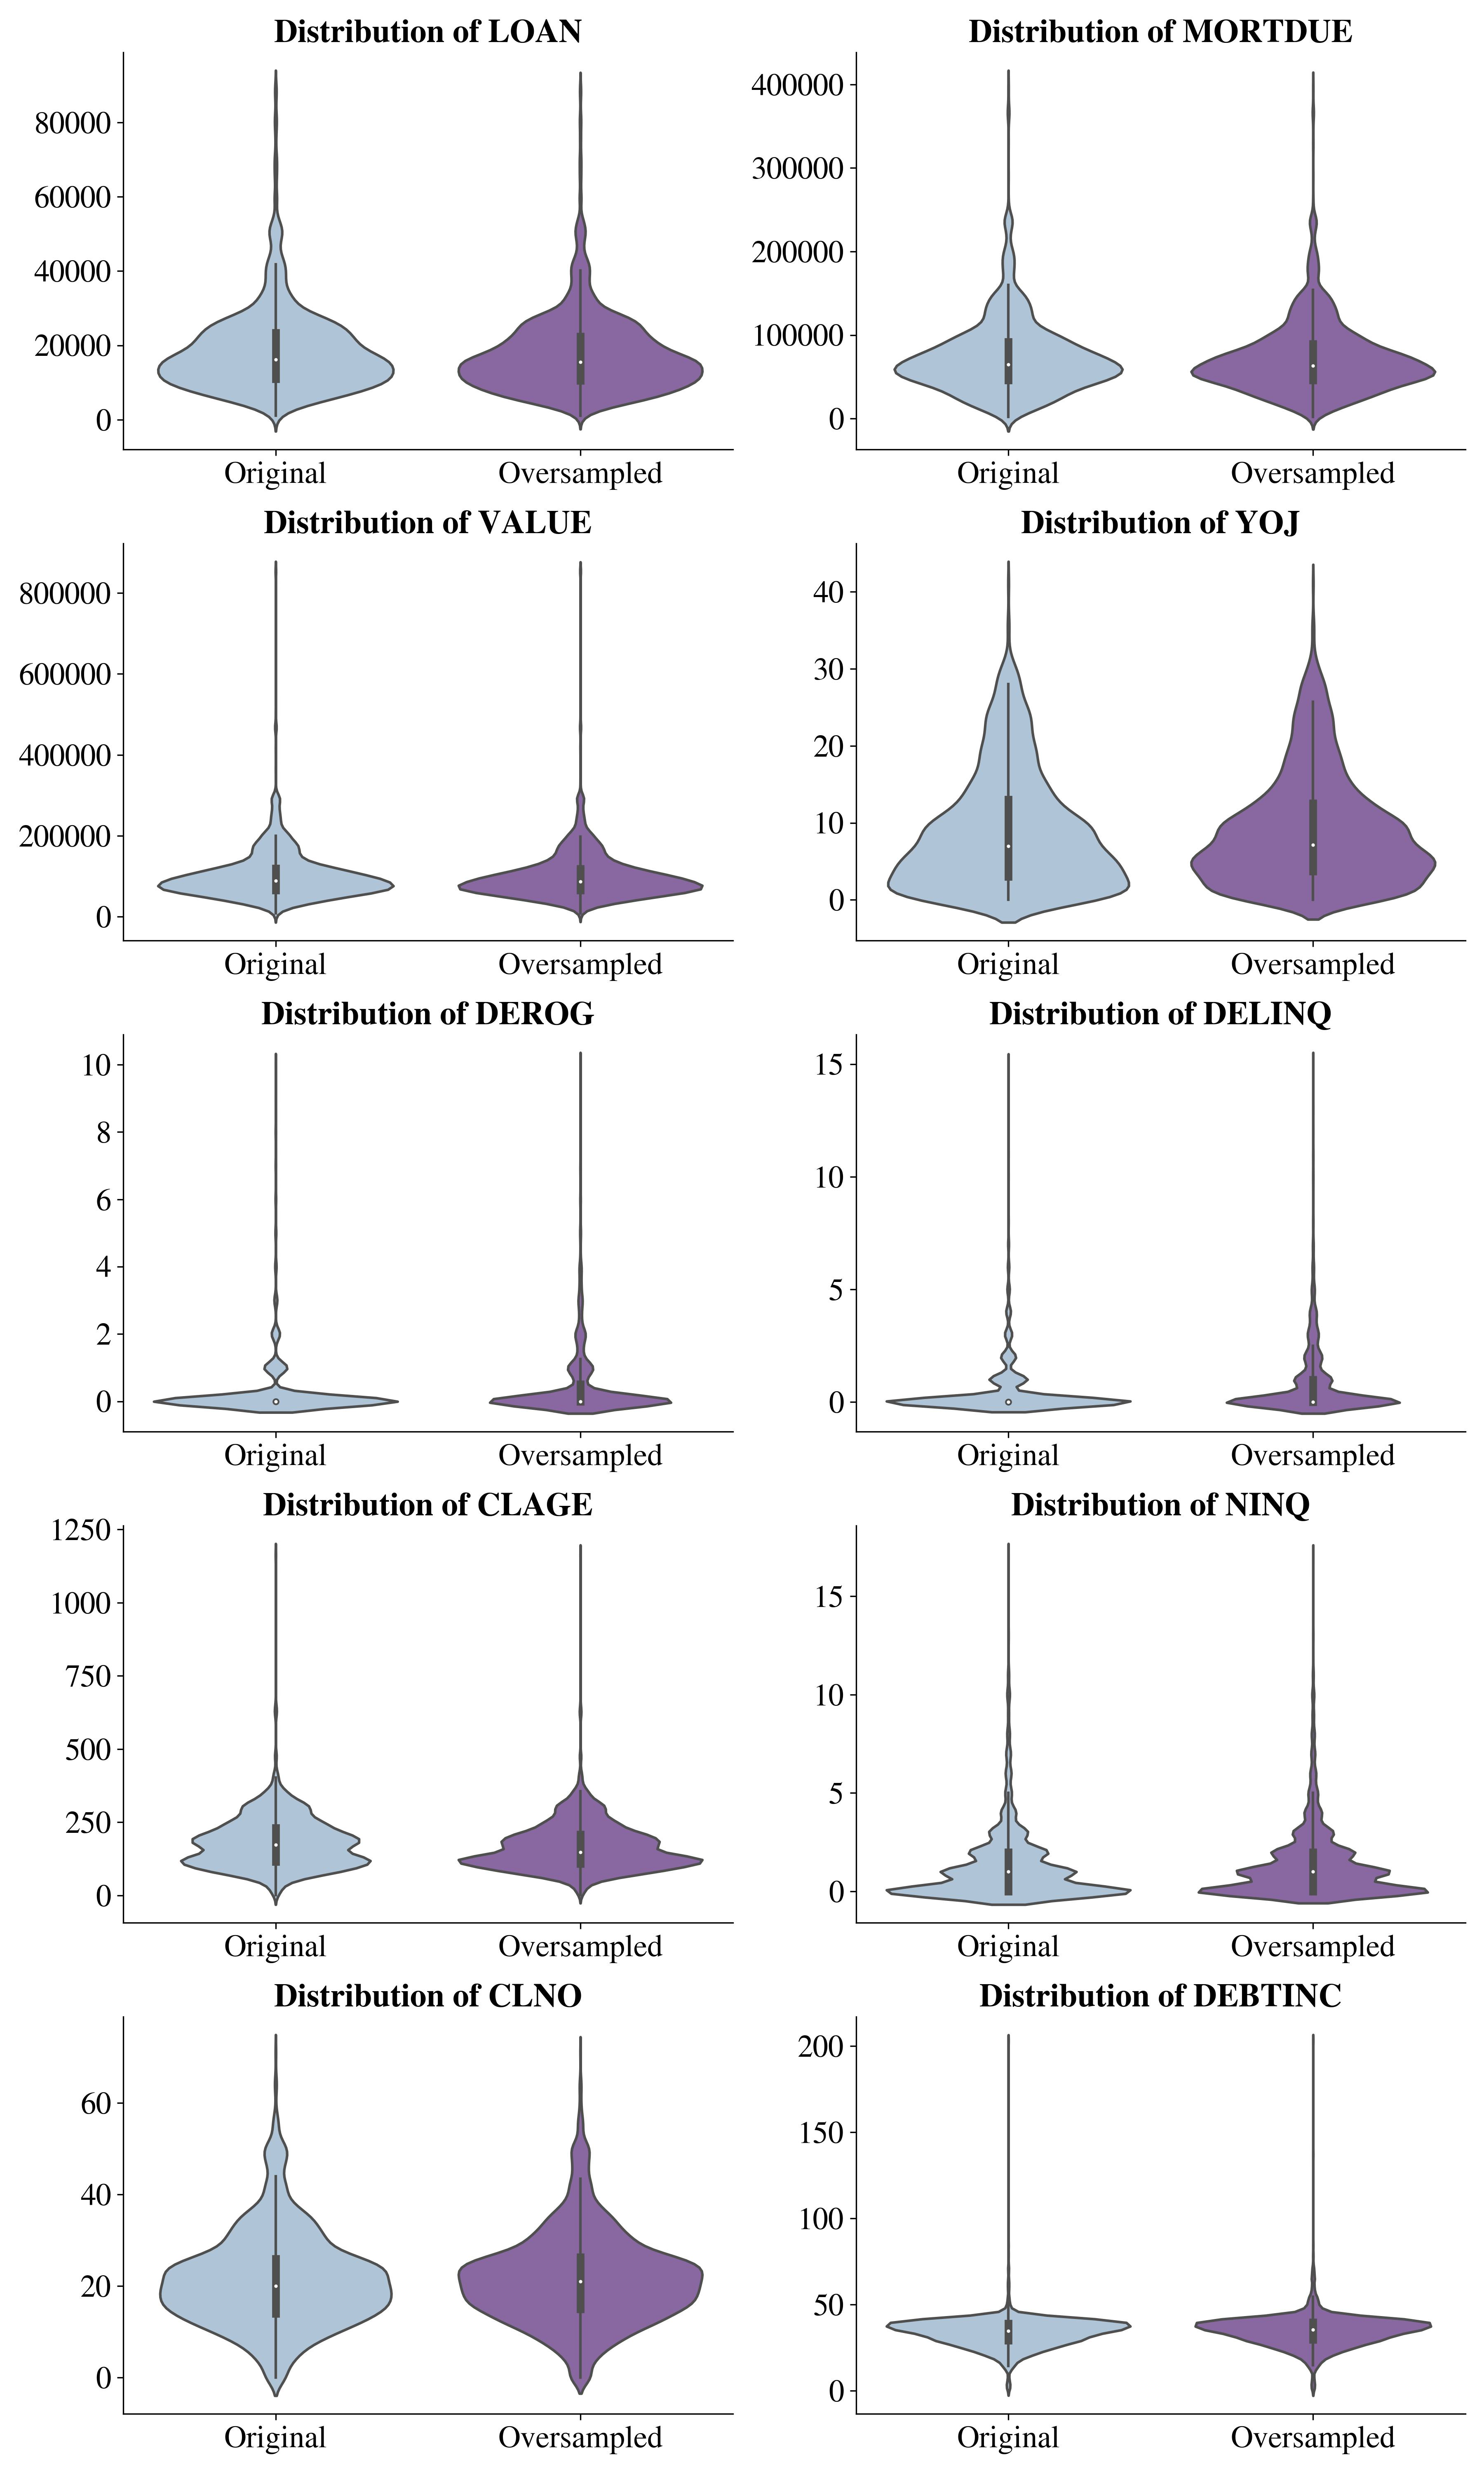
\includegraphics[width=140mm]{Figures/Numeric_Features_Distribution_OS_Violinplots.jpg}
    
    \centering{\begin{source}Author's results in Python\end{source}}\vspace{-1em}
\end{figure}


\begin{figure}[H]
    \centering
    \caption{WoE Bins Distribution}\vspace{0.5em}
    \label{fig:woedist}
    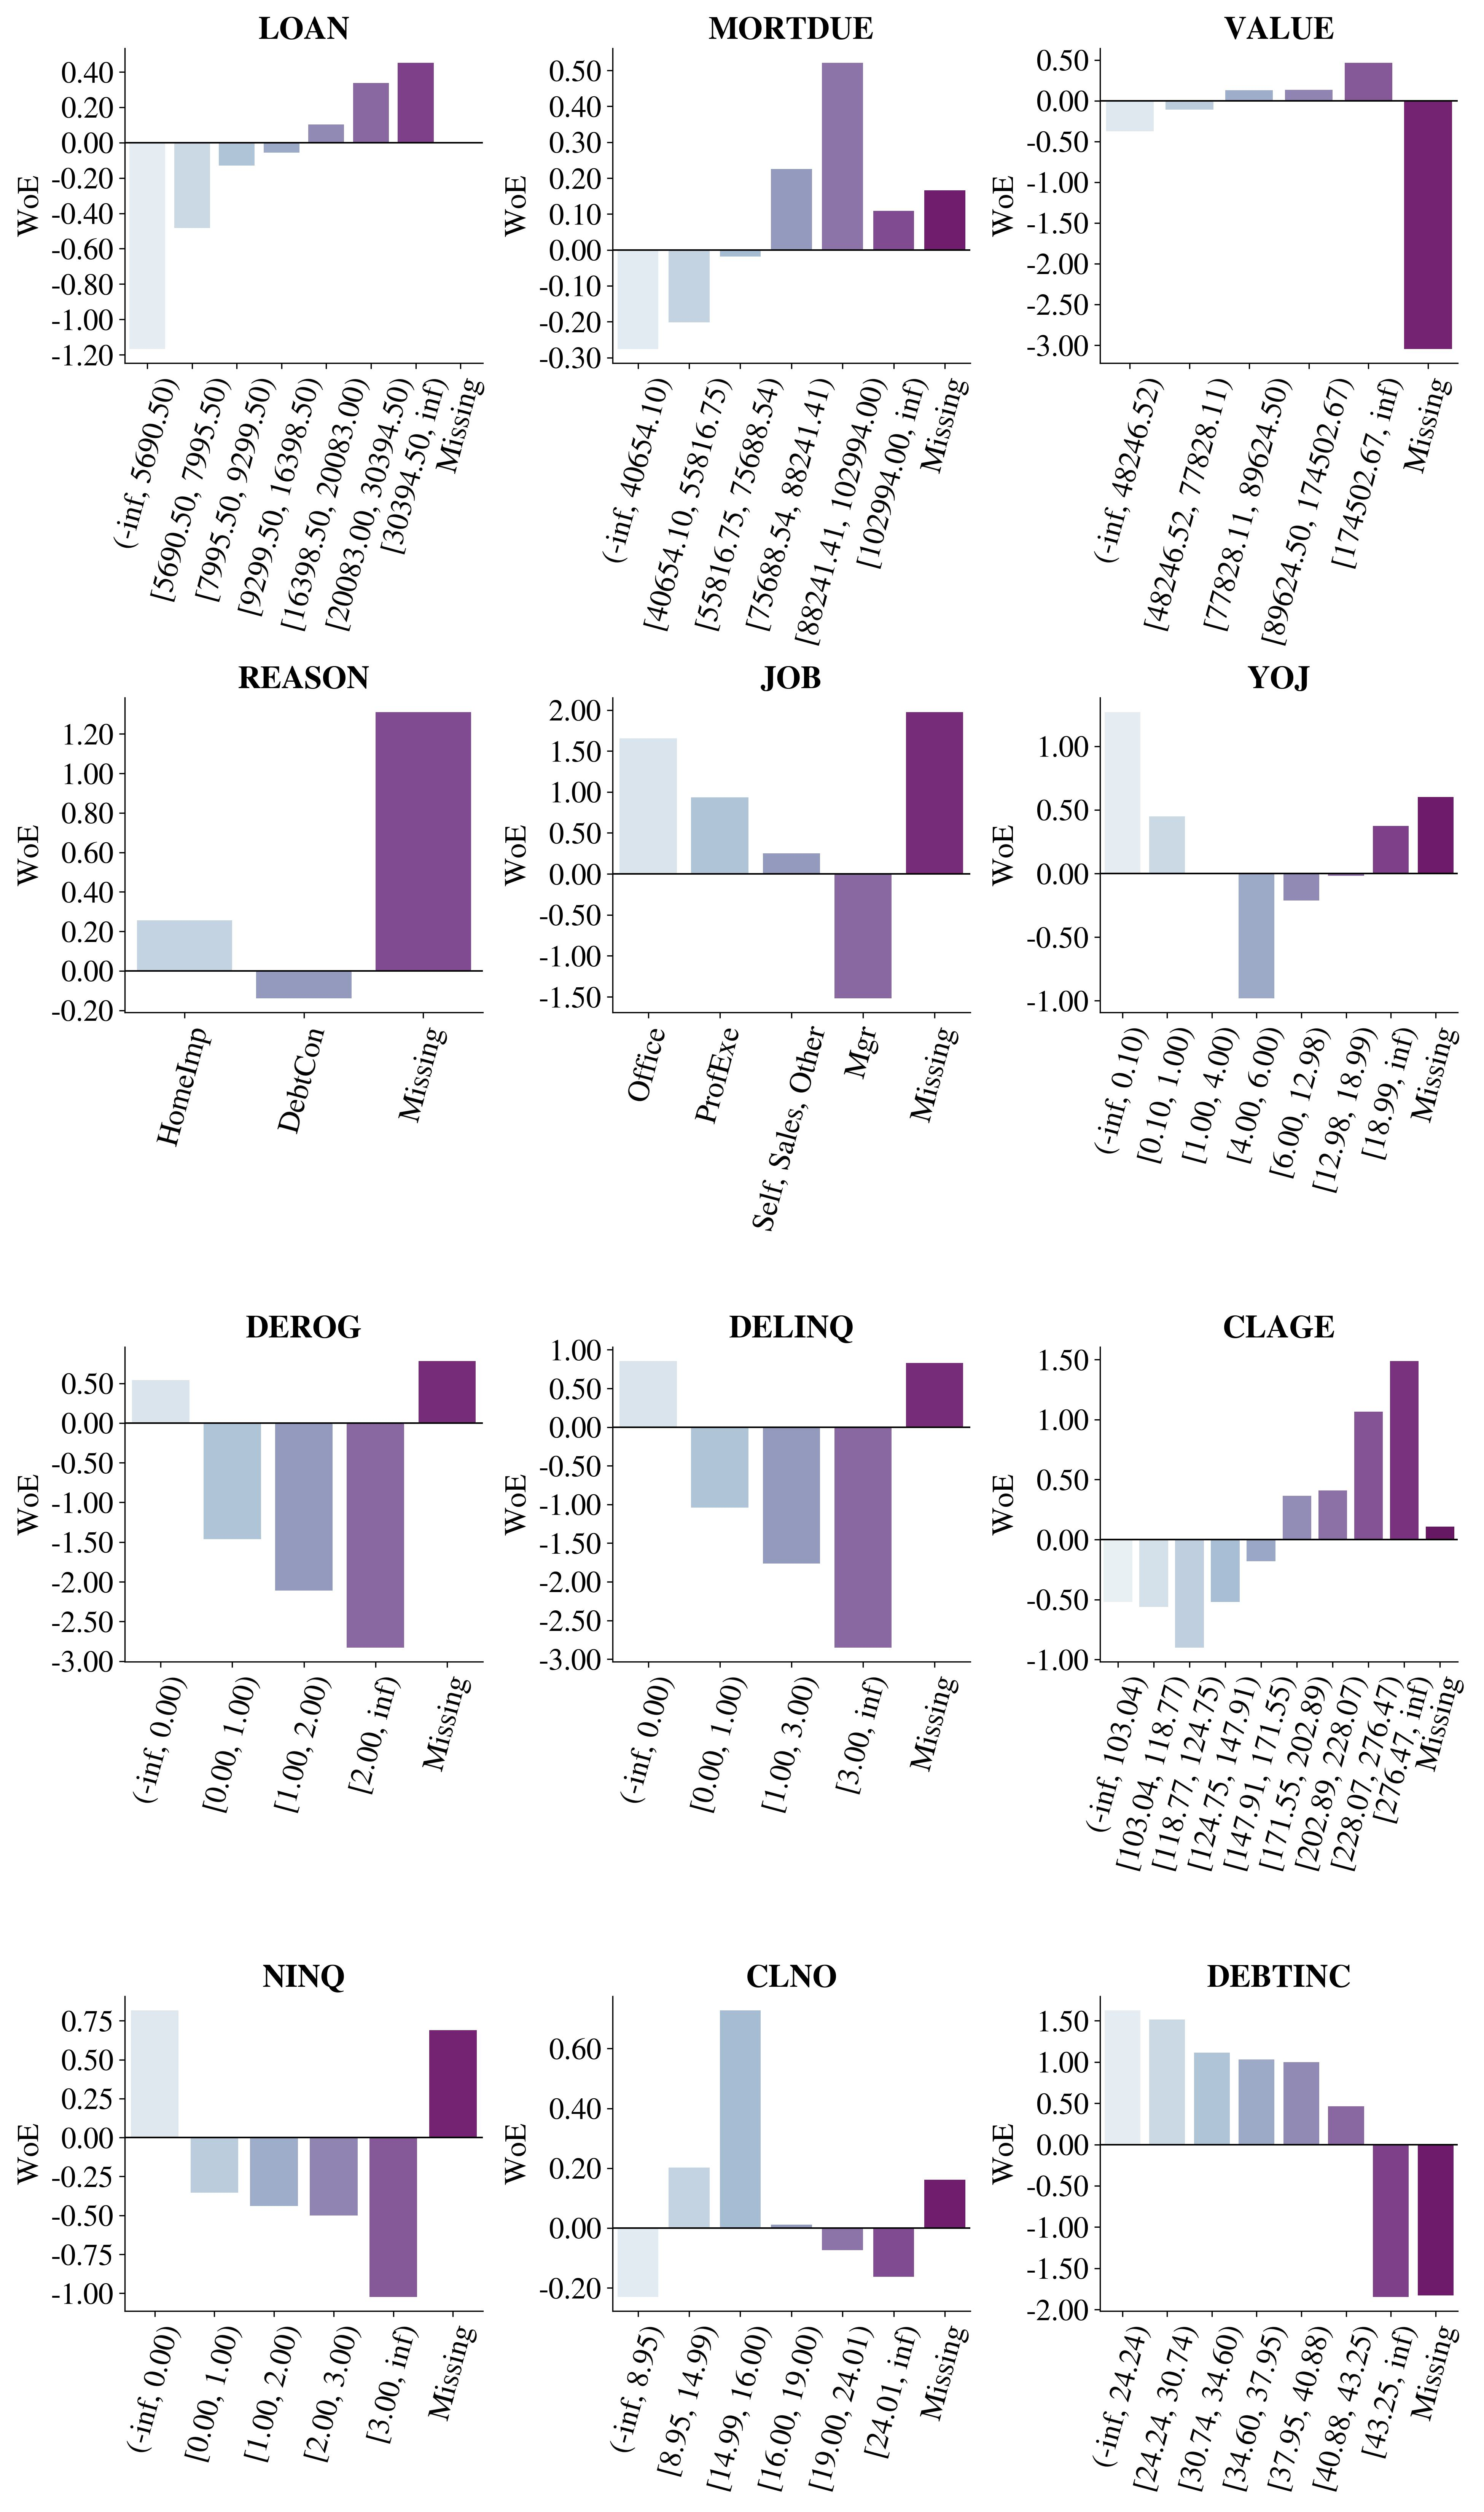
\includegraphics[width=100mm]{Figures/WoE_Distribution.jpg}
    
    \centering{\begin{source}Author's results in Python\end{source}}\vspace{-1em}
\end{figure}

\section{Model Selection Results}
\label{sec:app1modelselectionresultsapp}


\begin{figure}[H]
    \centering
    \caption{Special Case of KNN - Probability Scores Distribution (Training Set)}\vspace{0.5em}
    \label{fig:knndist}\
    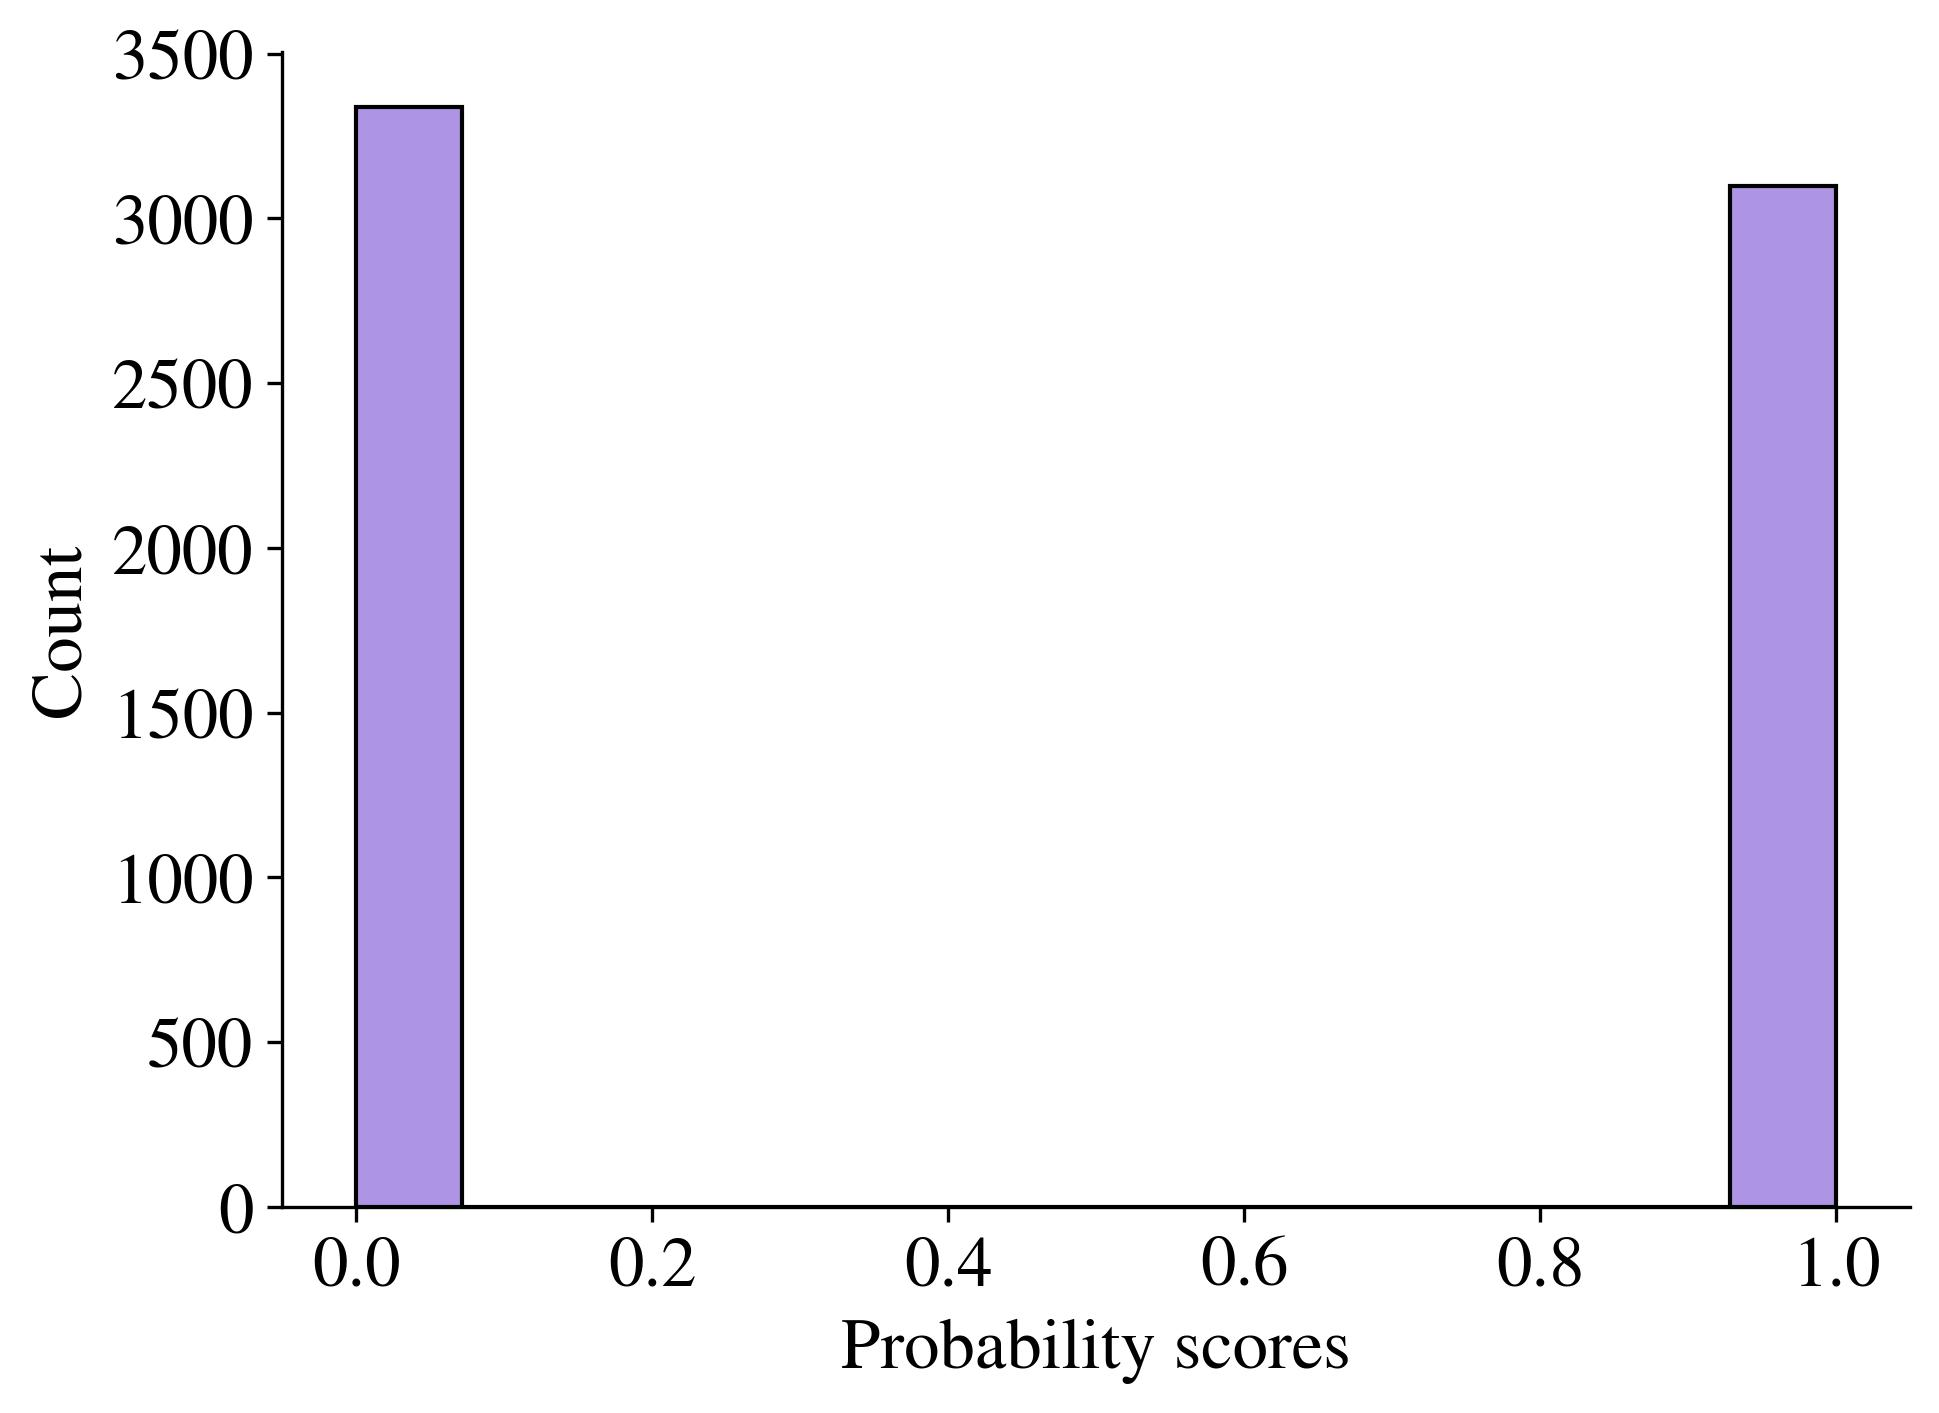
\includegraphics[width=110mm]{Figures/KNN_special_prob.jpg}
    
    \centering{\begin{source}Author's results in Python\end{source}}\vspace{-1em}
\end{figure}



\begin{figure}[H]
    \centering
    \caption{Special Case of KNN - ROC Curve (Training Set)}\vspace{0.5em}
    \label{fig:knnroc}\
    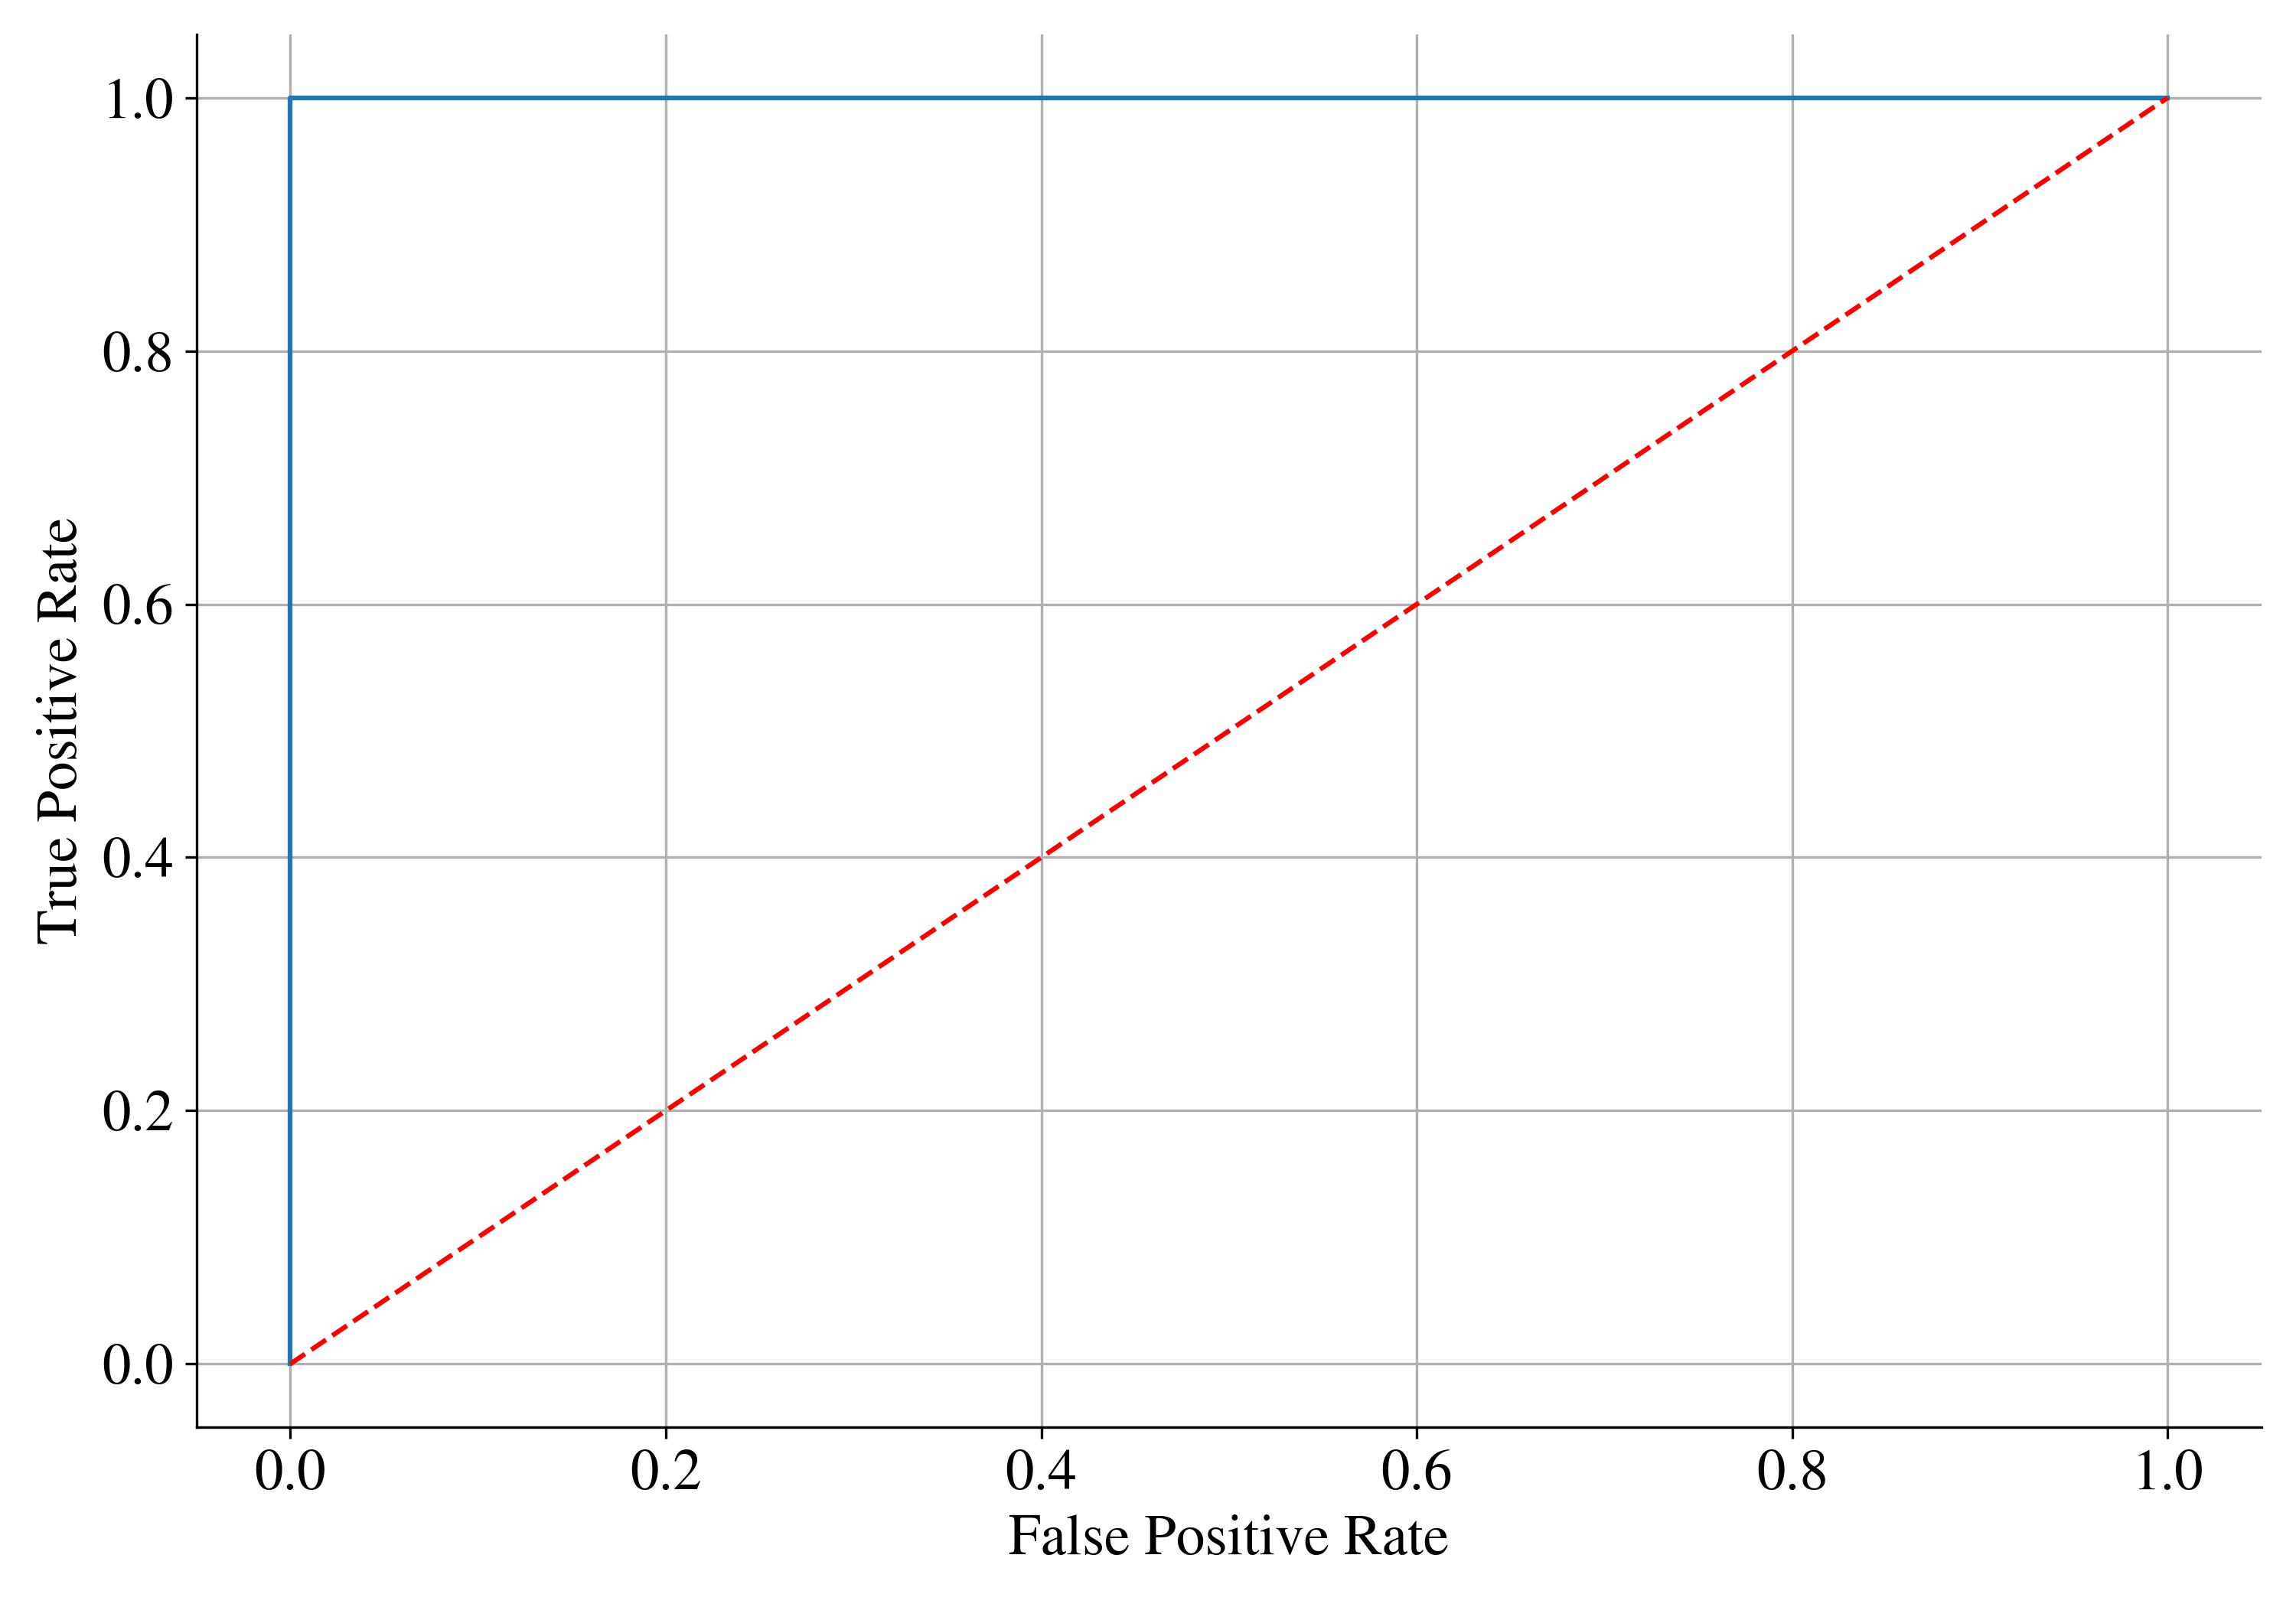
\includegraphics[width=140mm]{Figures/KNN_special_ROC.jpg}
    
    \centering{\begin{source}Author's results in Python\end{source}}\vspace{-1em}
\end{figure}



\begin{figure}[H]
    \centering
    \caption{Precision Distribution}\vspace{0.5em}
    \label{fig:precdist}
    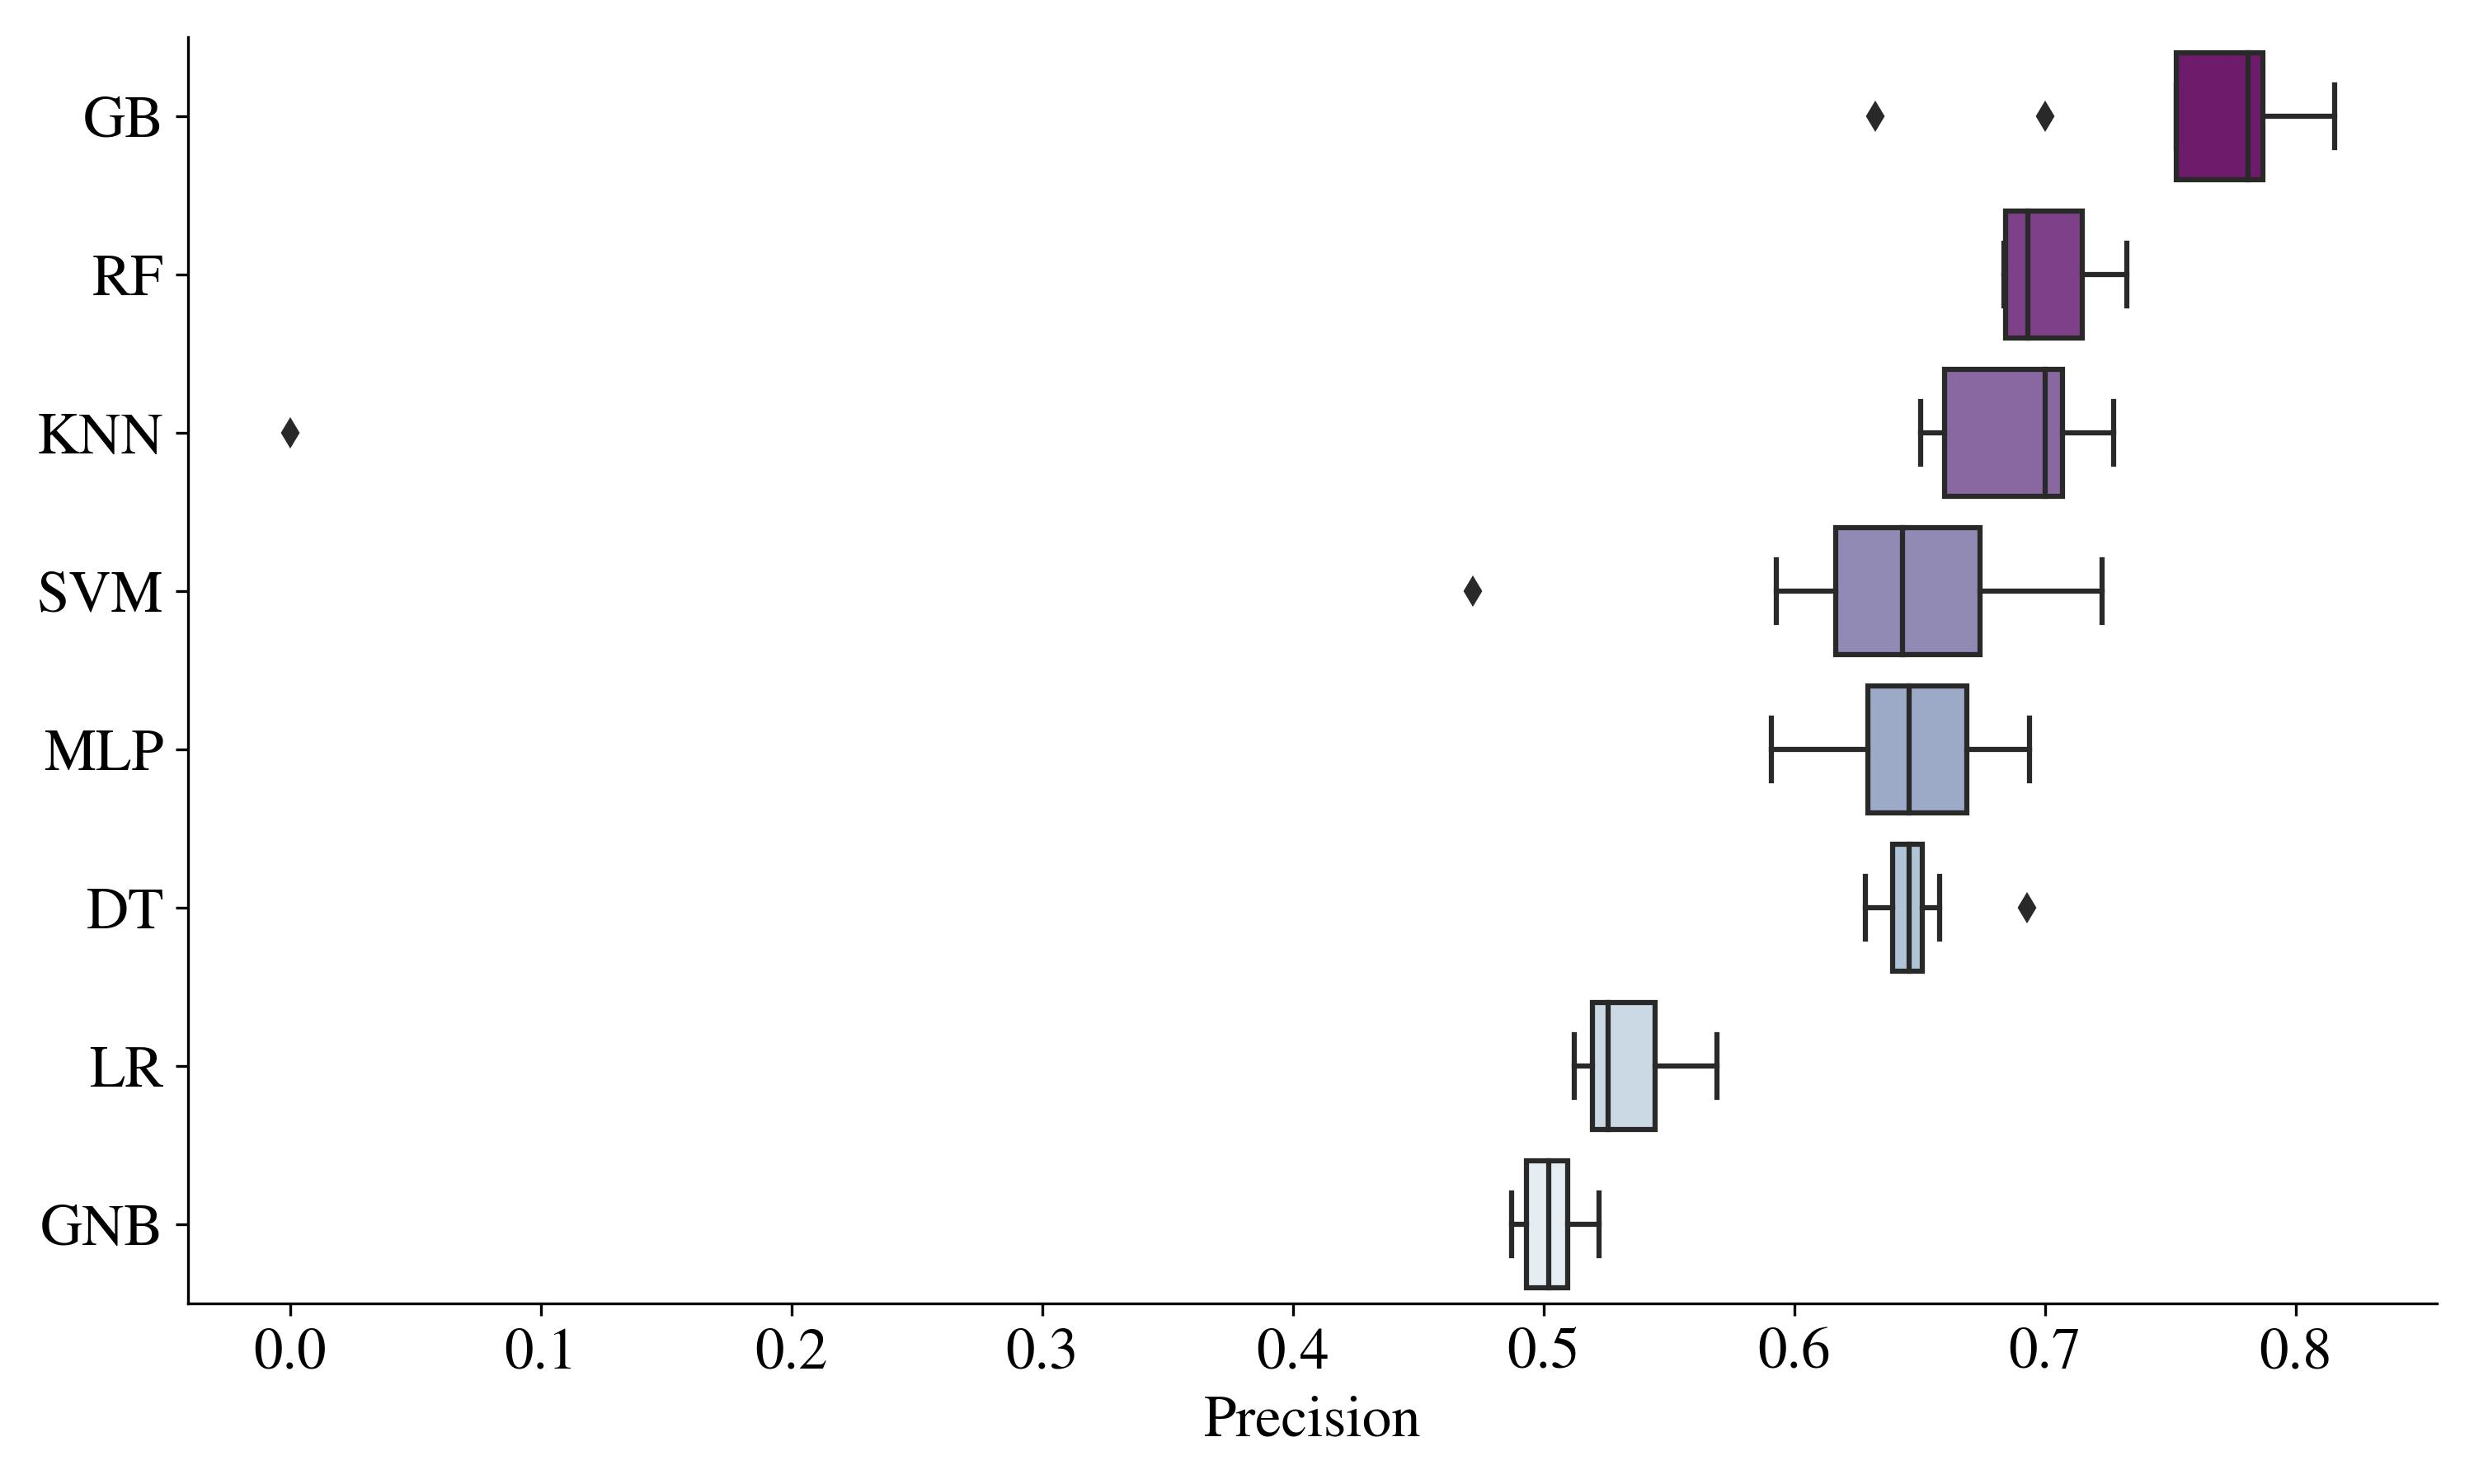
\includegraphics[width=140mm]{Figures/PRECISION_Distribution.jpg}
    
    \centering{\begin{source}Author's results in Python\end{source}}\vspace{-1em}
\end{figure}

\begin{figure}[H]
    \centering
    \caption{Precision Distribution - \textit{without outlier}}\vspace{0.5em}
    \label{fig:precdistwoout}
    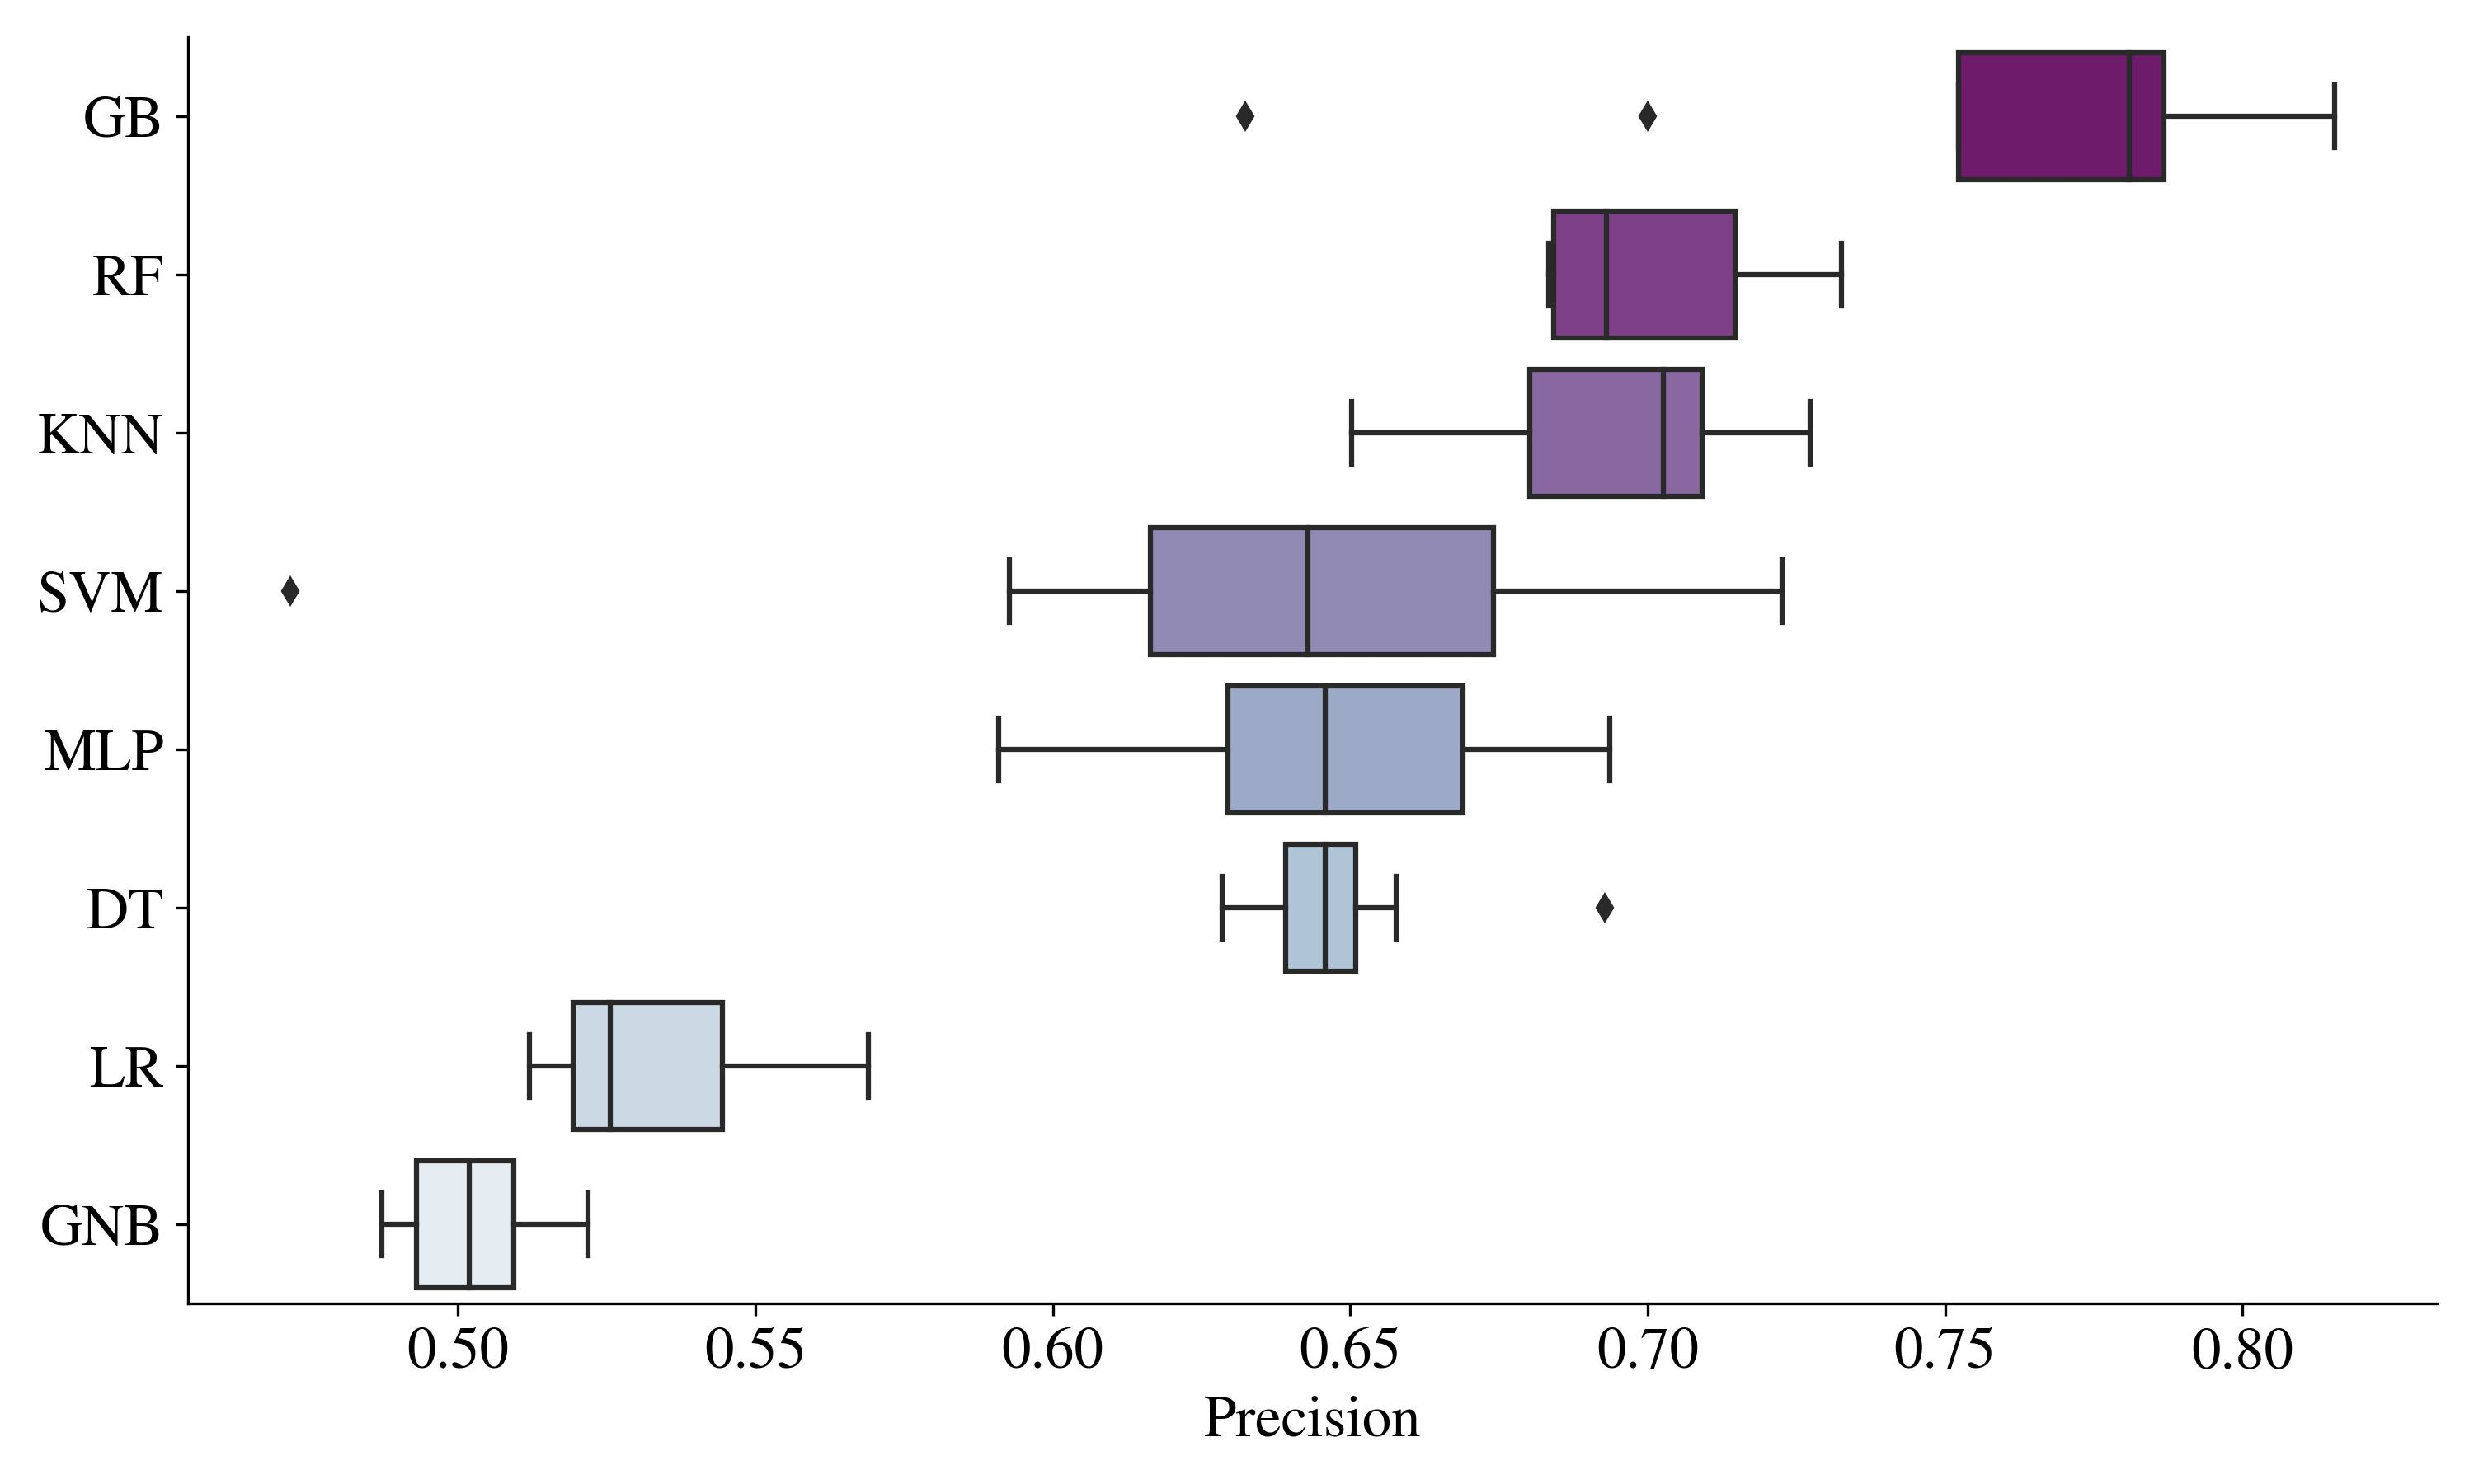
\includegraphics[width=140mm]{Figures/PRECISION_WO_OUTLIERS_Distribution.jpg}
    
    \centering{\begin{source}Author's results in Python\end{source}}\vspace{-1em}
\end{figure}

\begin{figure}[H]
    \centering
    \caption{Precision Distribution (Black--box/White--box dimension)}\vspace{0.5em}
    \label{fig:precdistbbwb}
    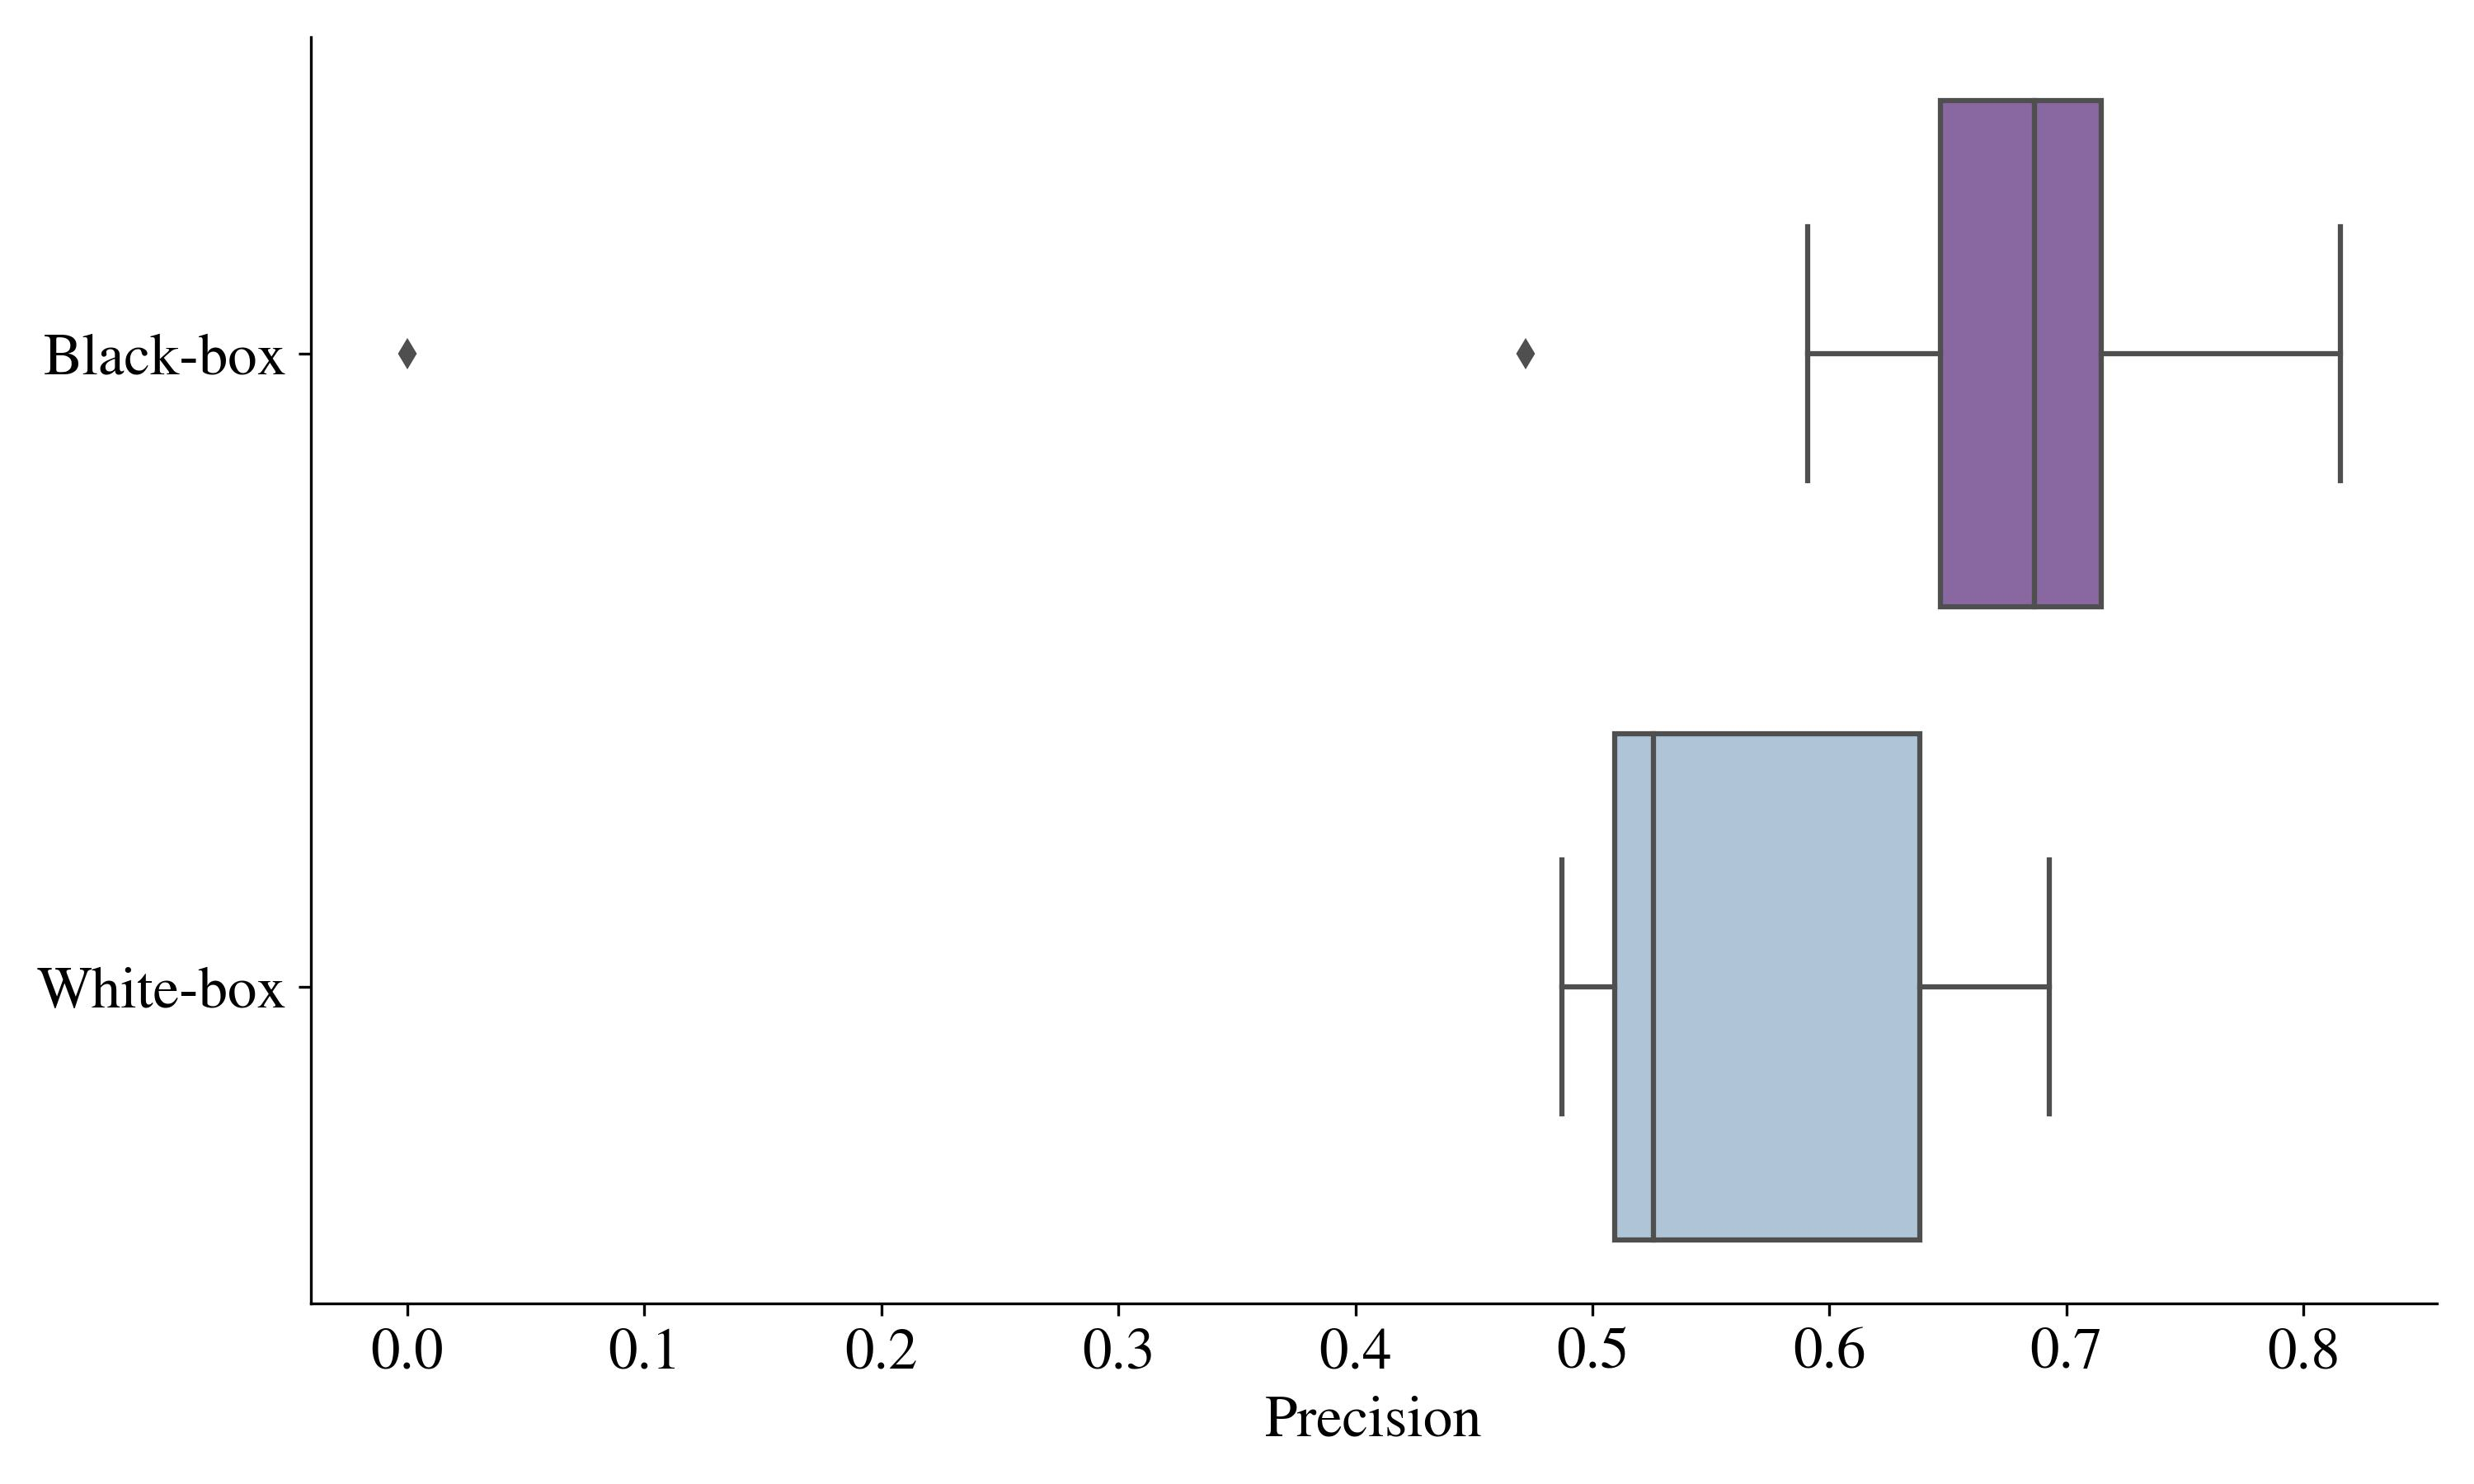
\includegraphics[width=140mm]{Figures/PRECISION_Distribution_BB_WB.jpg}
    
    \centering{\begin{source}Author's results in Python\end{source}}\vspace{-1em}
\end{figure}

\begin{figure}[H]
    \centering
    \caption{Precision Distribution (Black--box/White--box dimension) - \textit{without outlier}}\vspace{0.5em}
    \label{fig:precdistwooutbbwb}
    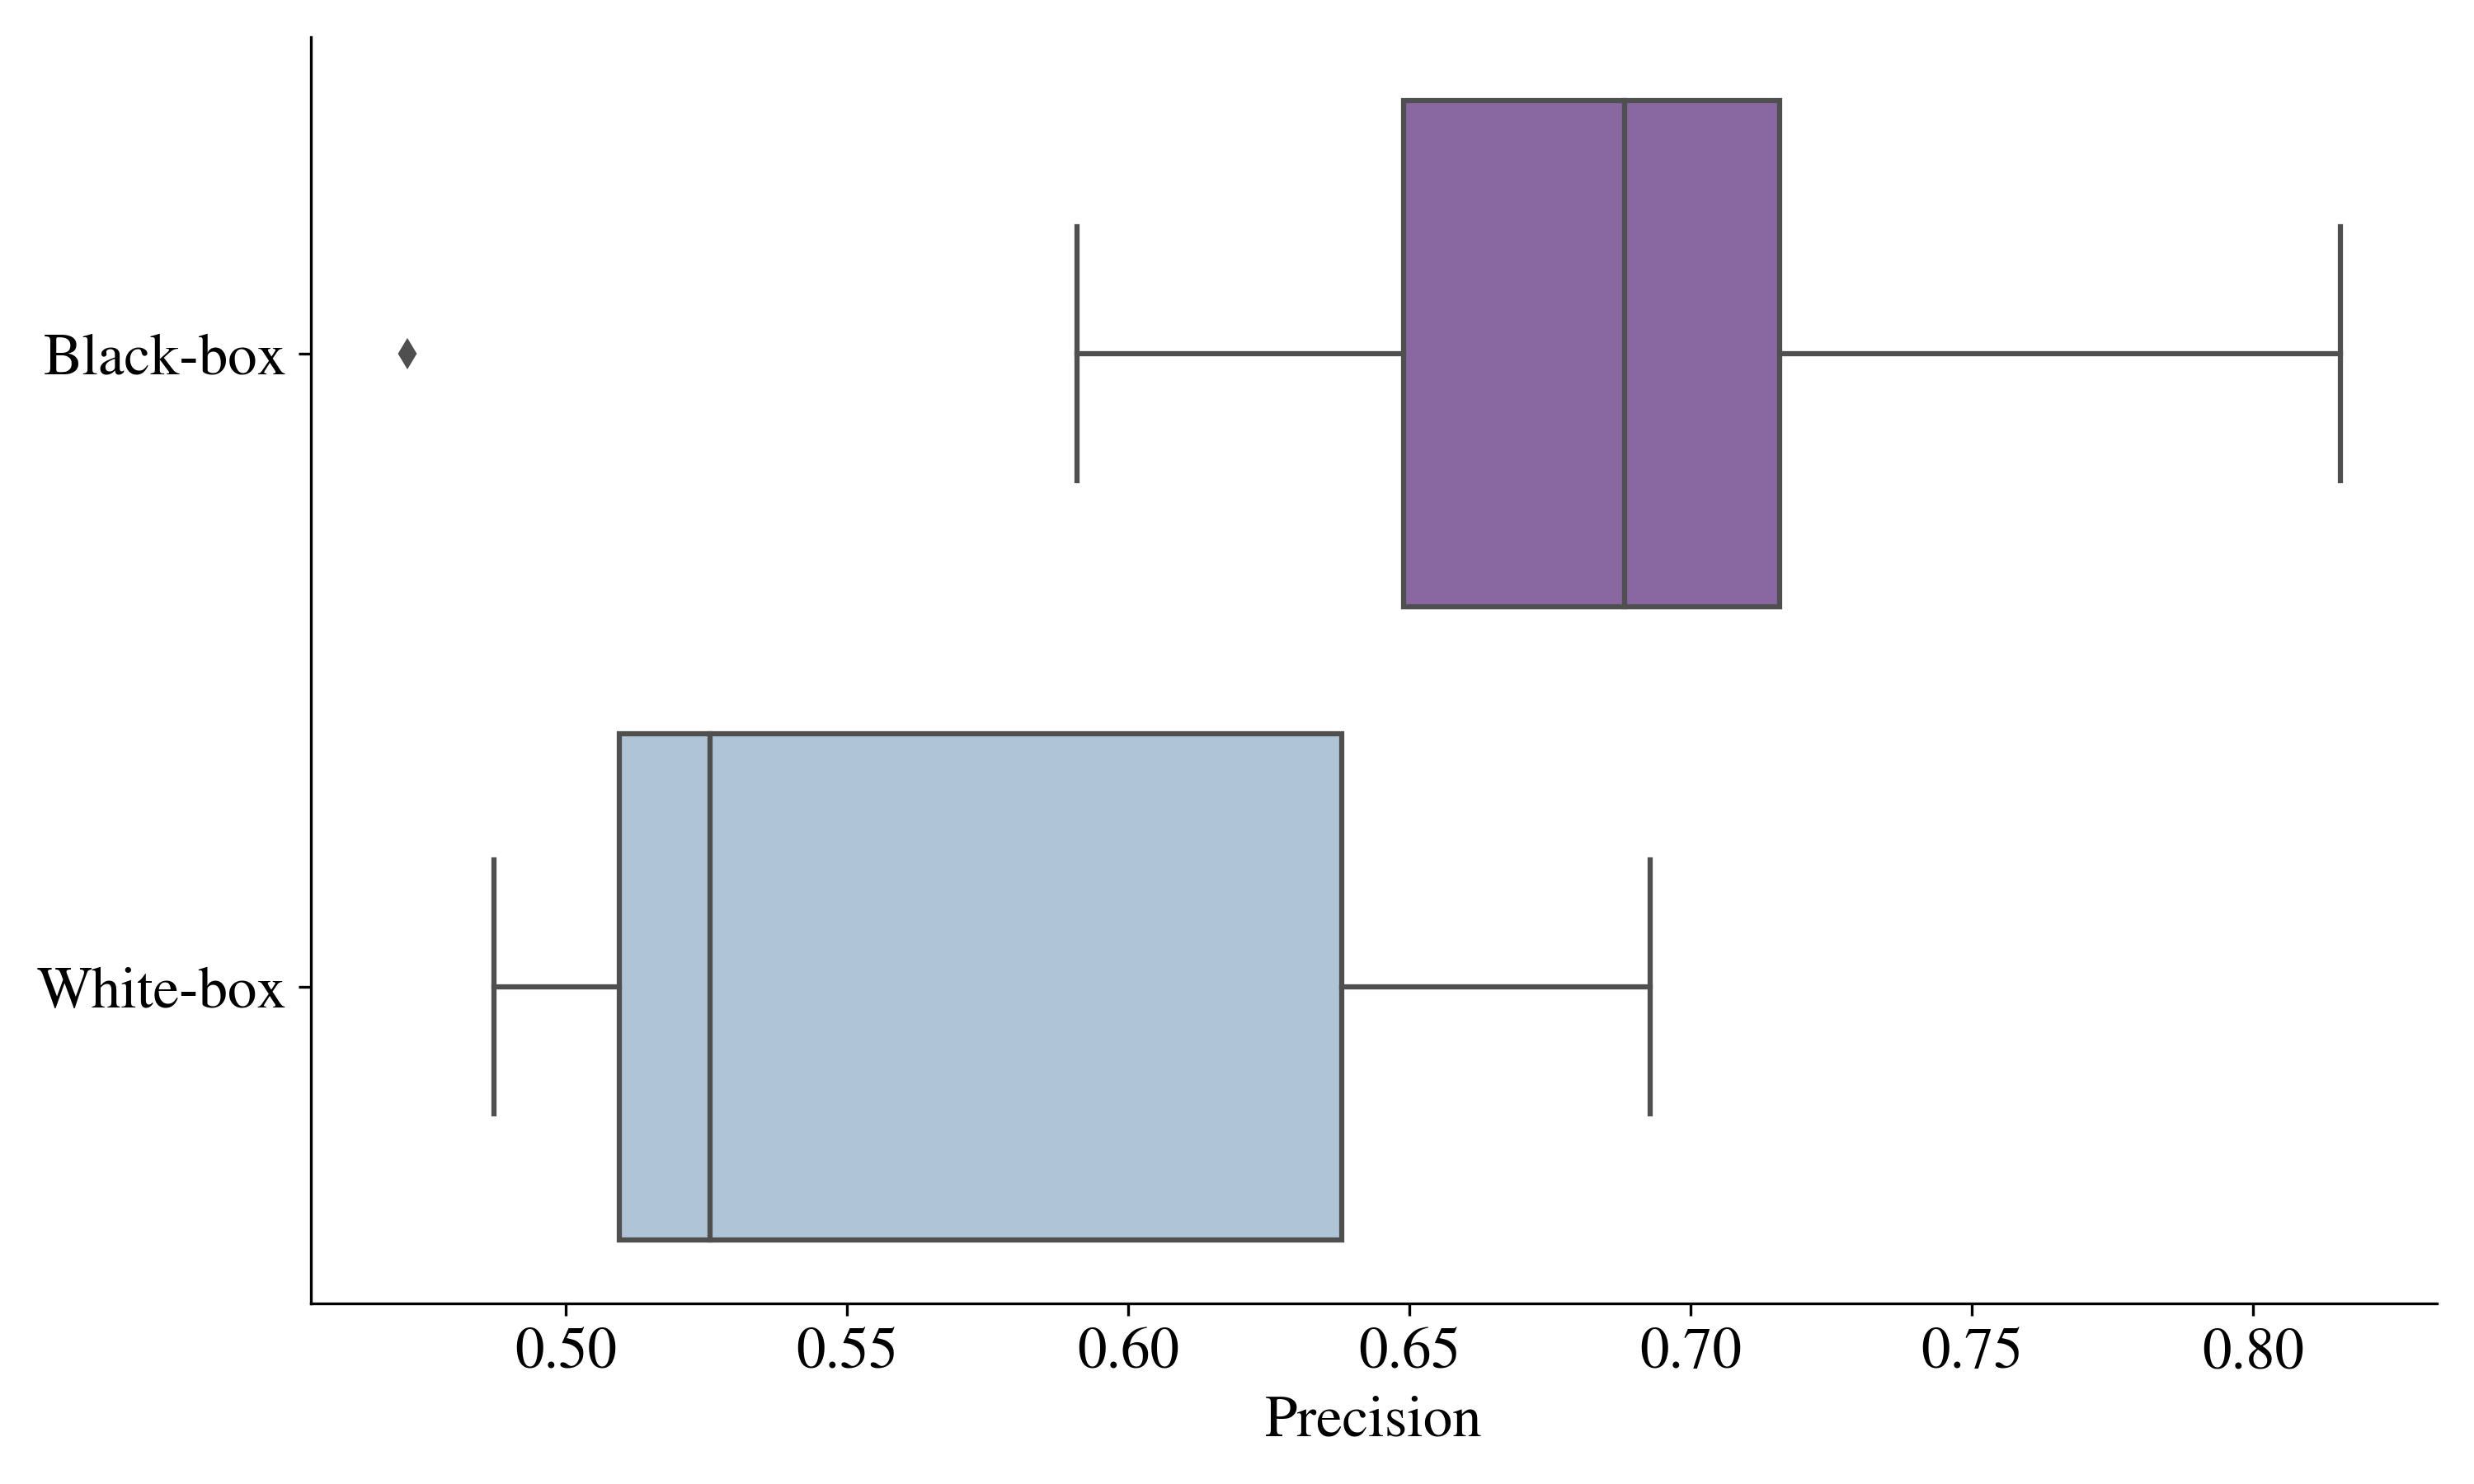
\includegraphics[width=140mm]{Figures/PRECISION_WO_OUTLIERS_Distribution_BB_WB.jpg}
    
    \centering{\begin{source}Author's results in Python\end{source}}\vspace{-1em}
\end{figure}



\begin{figure}[H]
    \centering
    \caption{Recall Distribution}\vspace{0.5em}
    \label{fig:reccdist}
    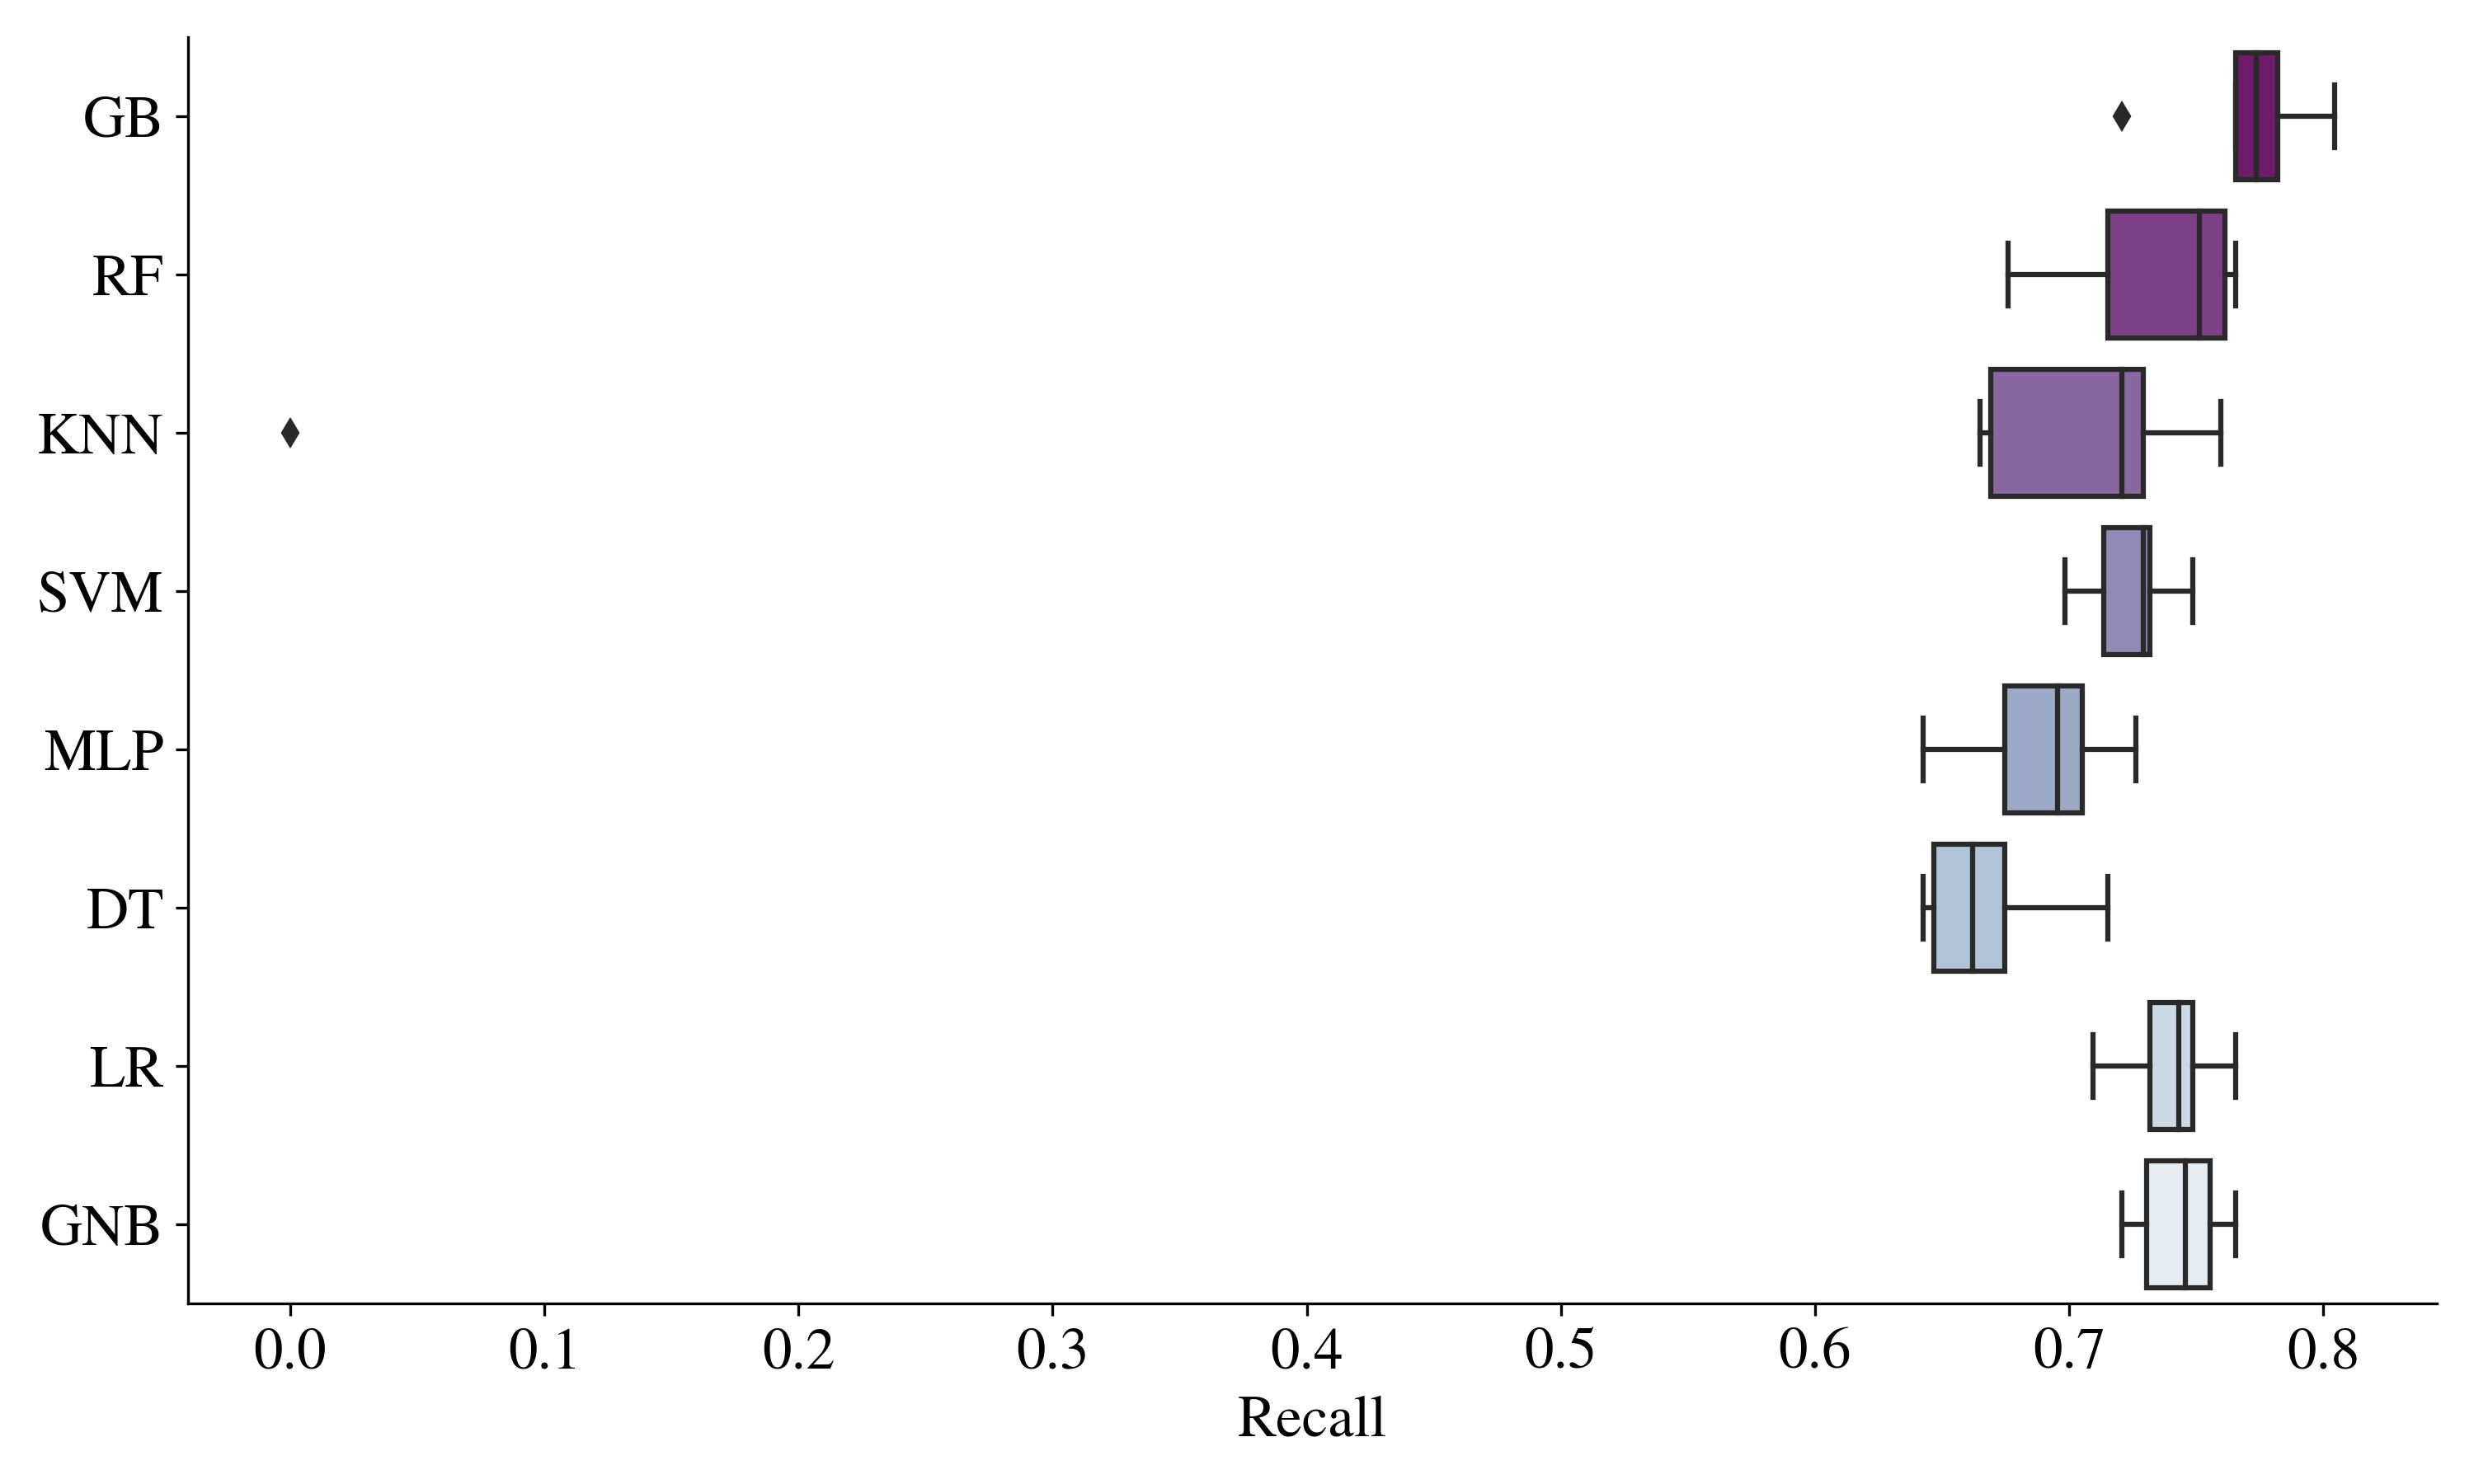
\includegraphics[width=140mm]{Figures/RECALL_Distribution.jpg}
    
    \centering{\begin{source}Author's results in Python\end{source}}\vspace{-1em}
\end{figure}

\begin{figure}[H]
    \centering
    \caption{Recall Distribution - \textit{without outlier}}\vspace{0.5em}
    \label{fig:recdistwoout}
    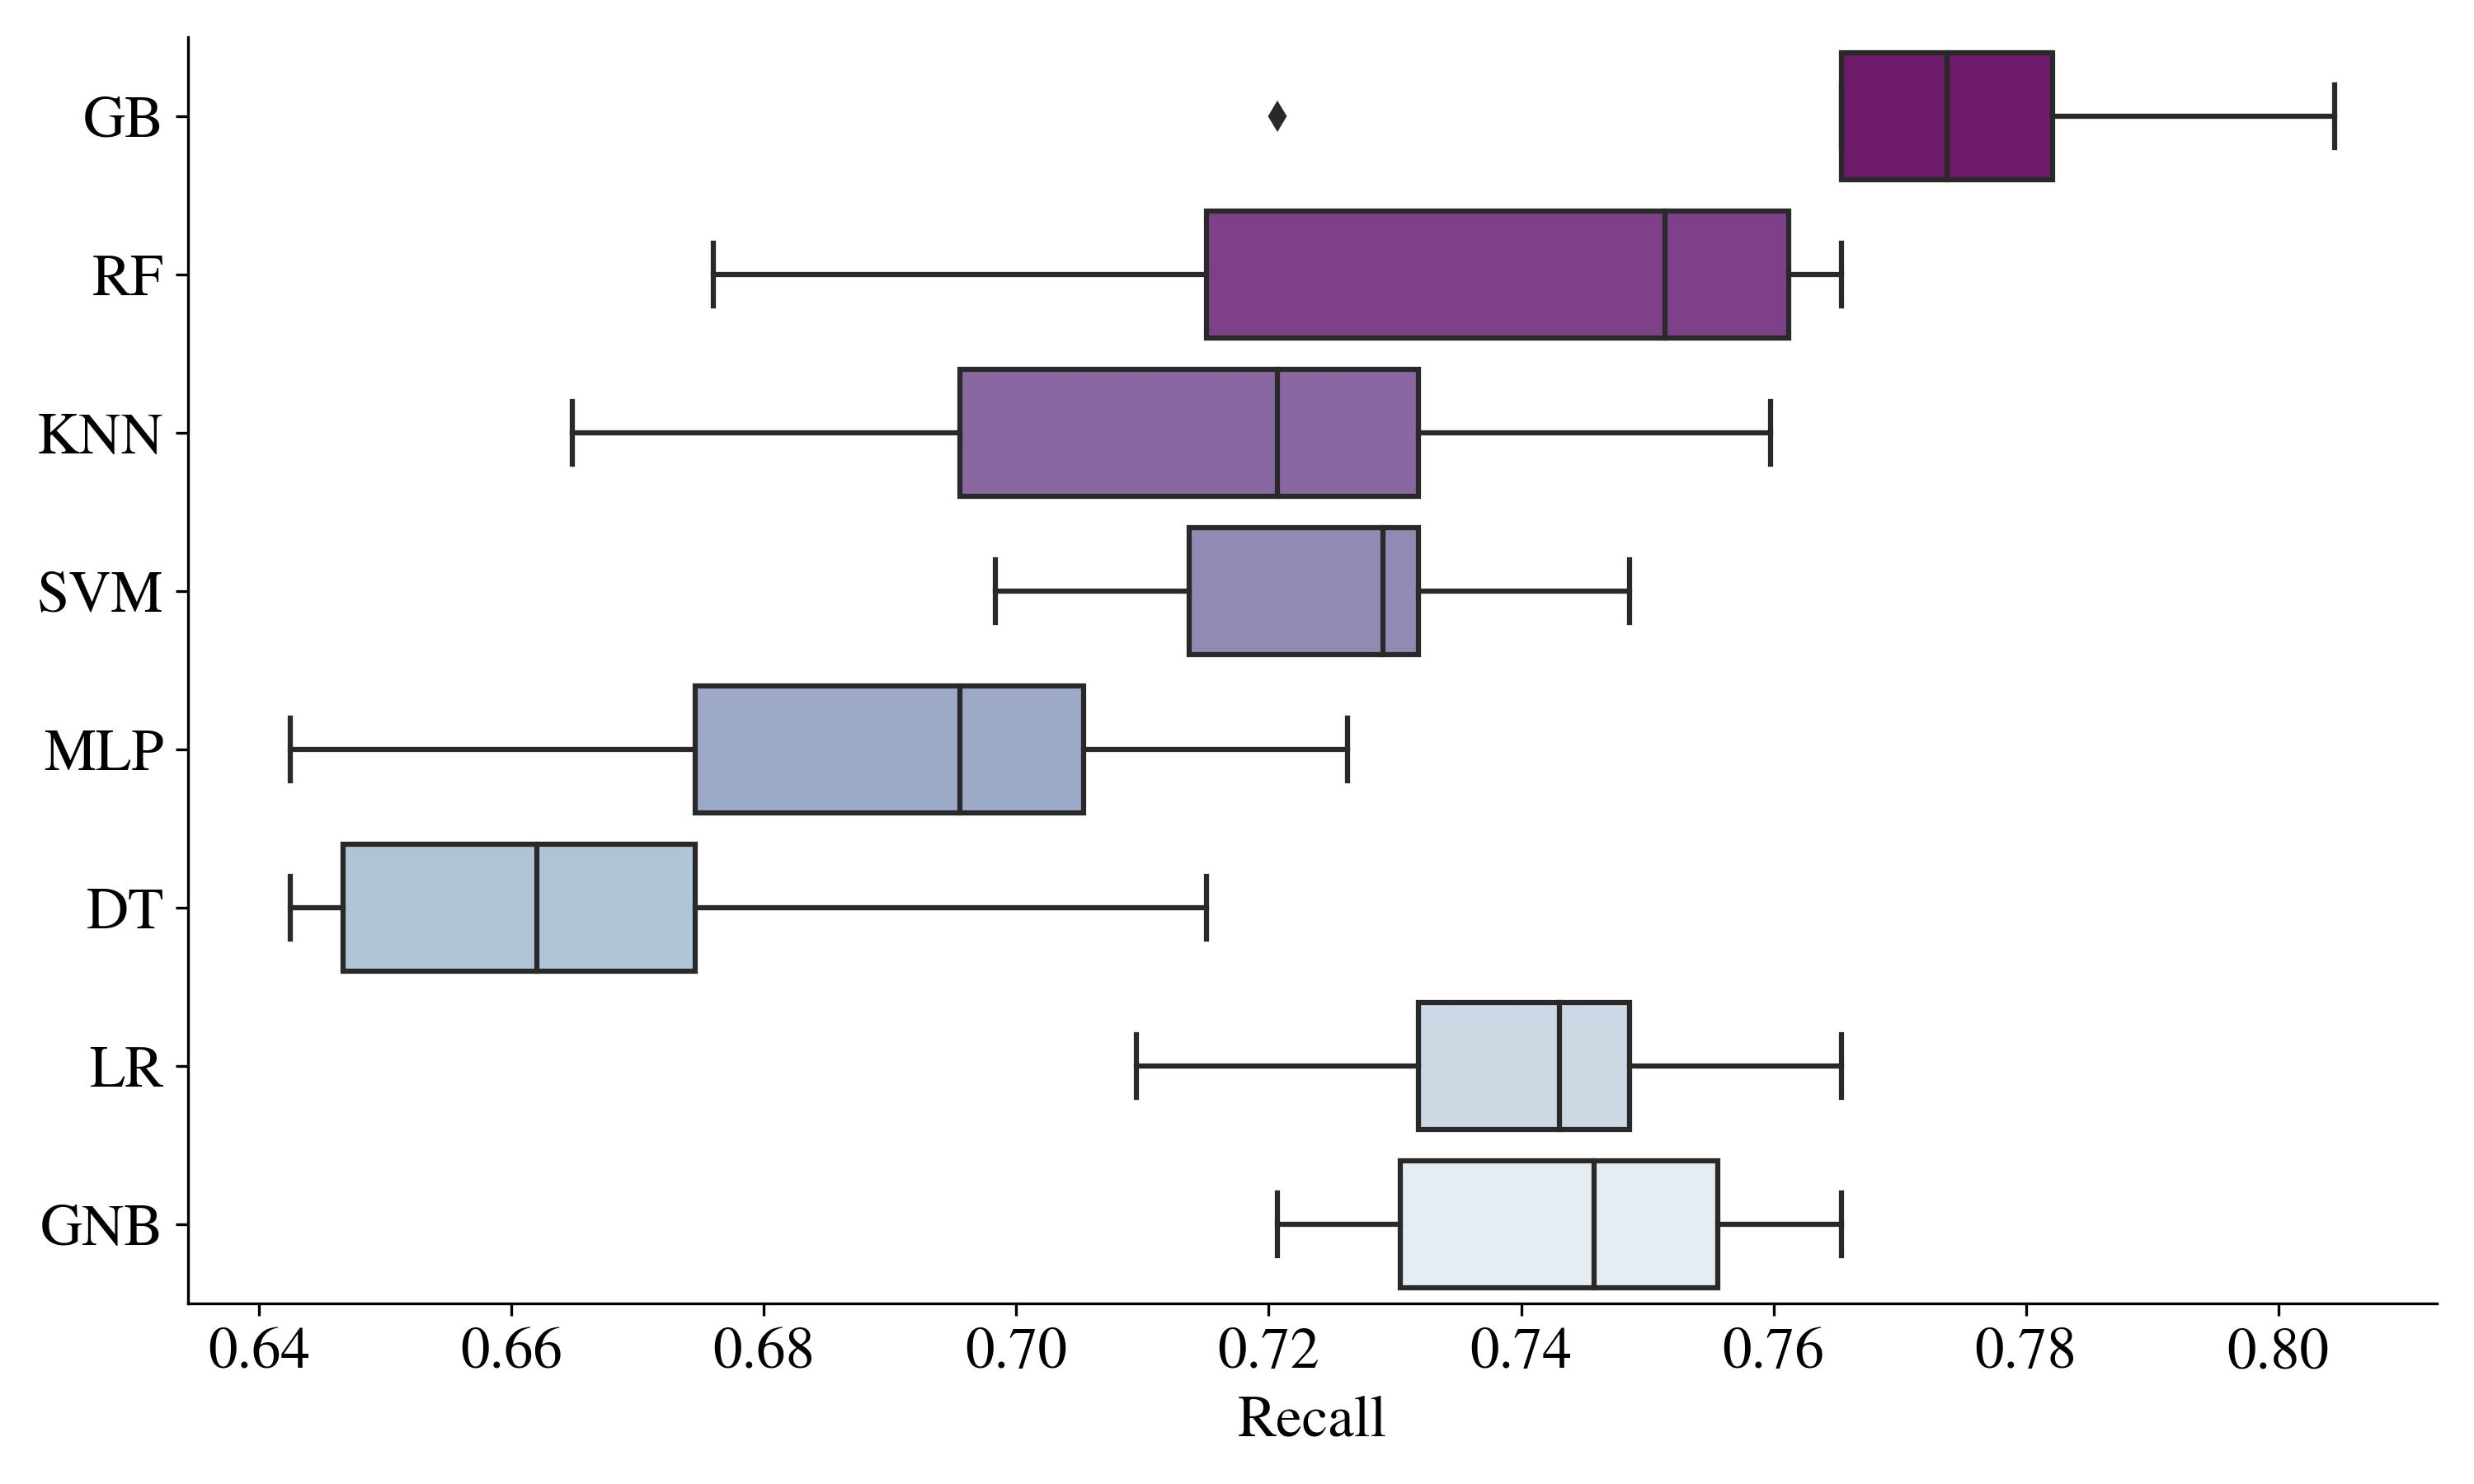
\includegraphics[width=140mm]{Figures/RECALL_WO_OUTLIERS_Distribution.jpg}
    
    \centering{\begin{source}Author's results in Python\end{source}}\vspace{-1em}
\end{figure}

\begin{figure}[H]
    \centering
    \caption{Recall Distribution (Black--box/White--box dimension)}\vspace{0.5em}
    \label{fig:recdistbbwb}
    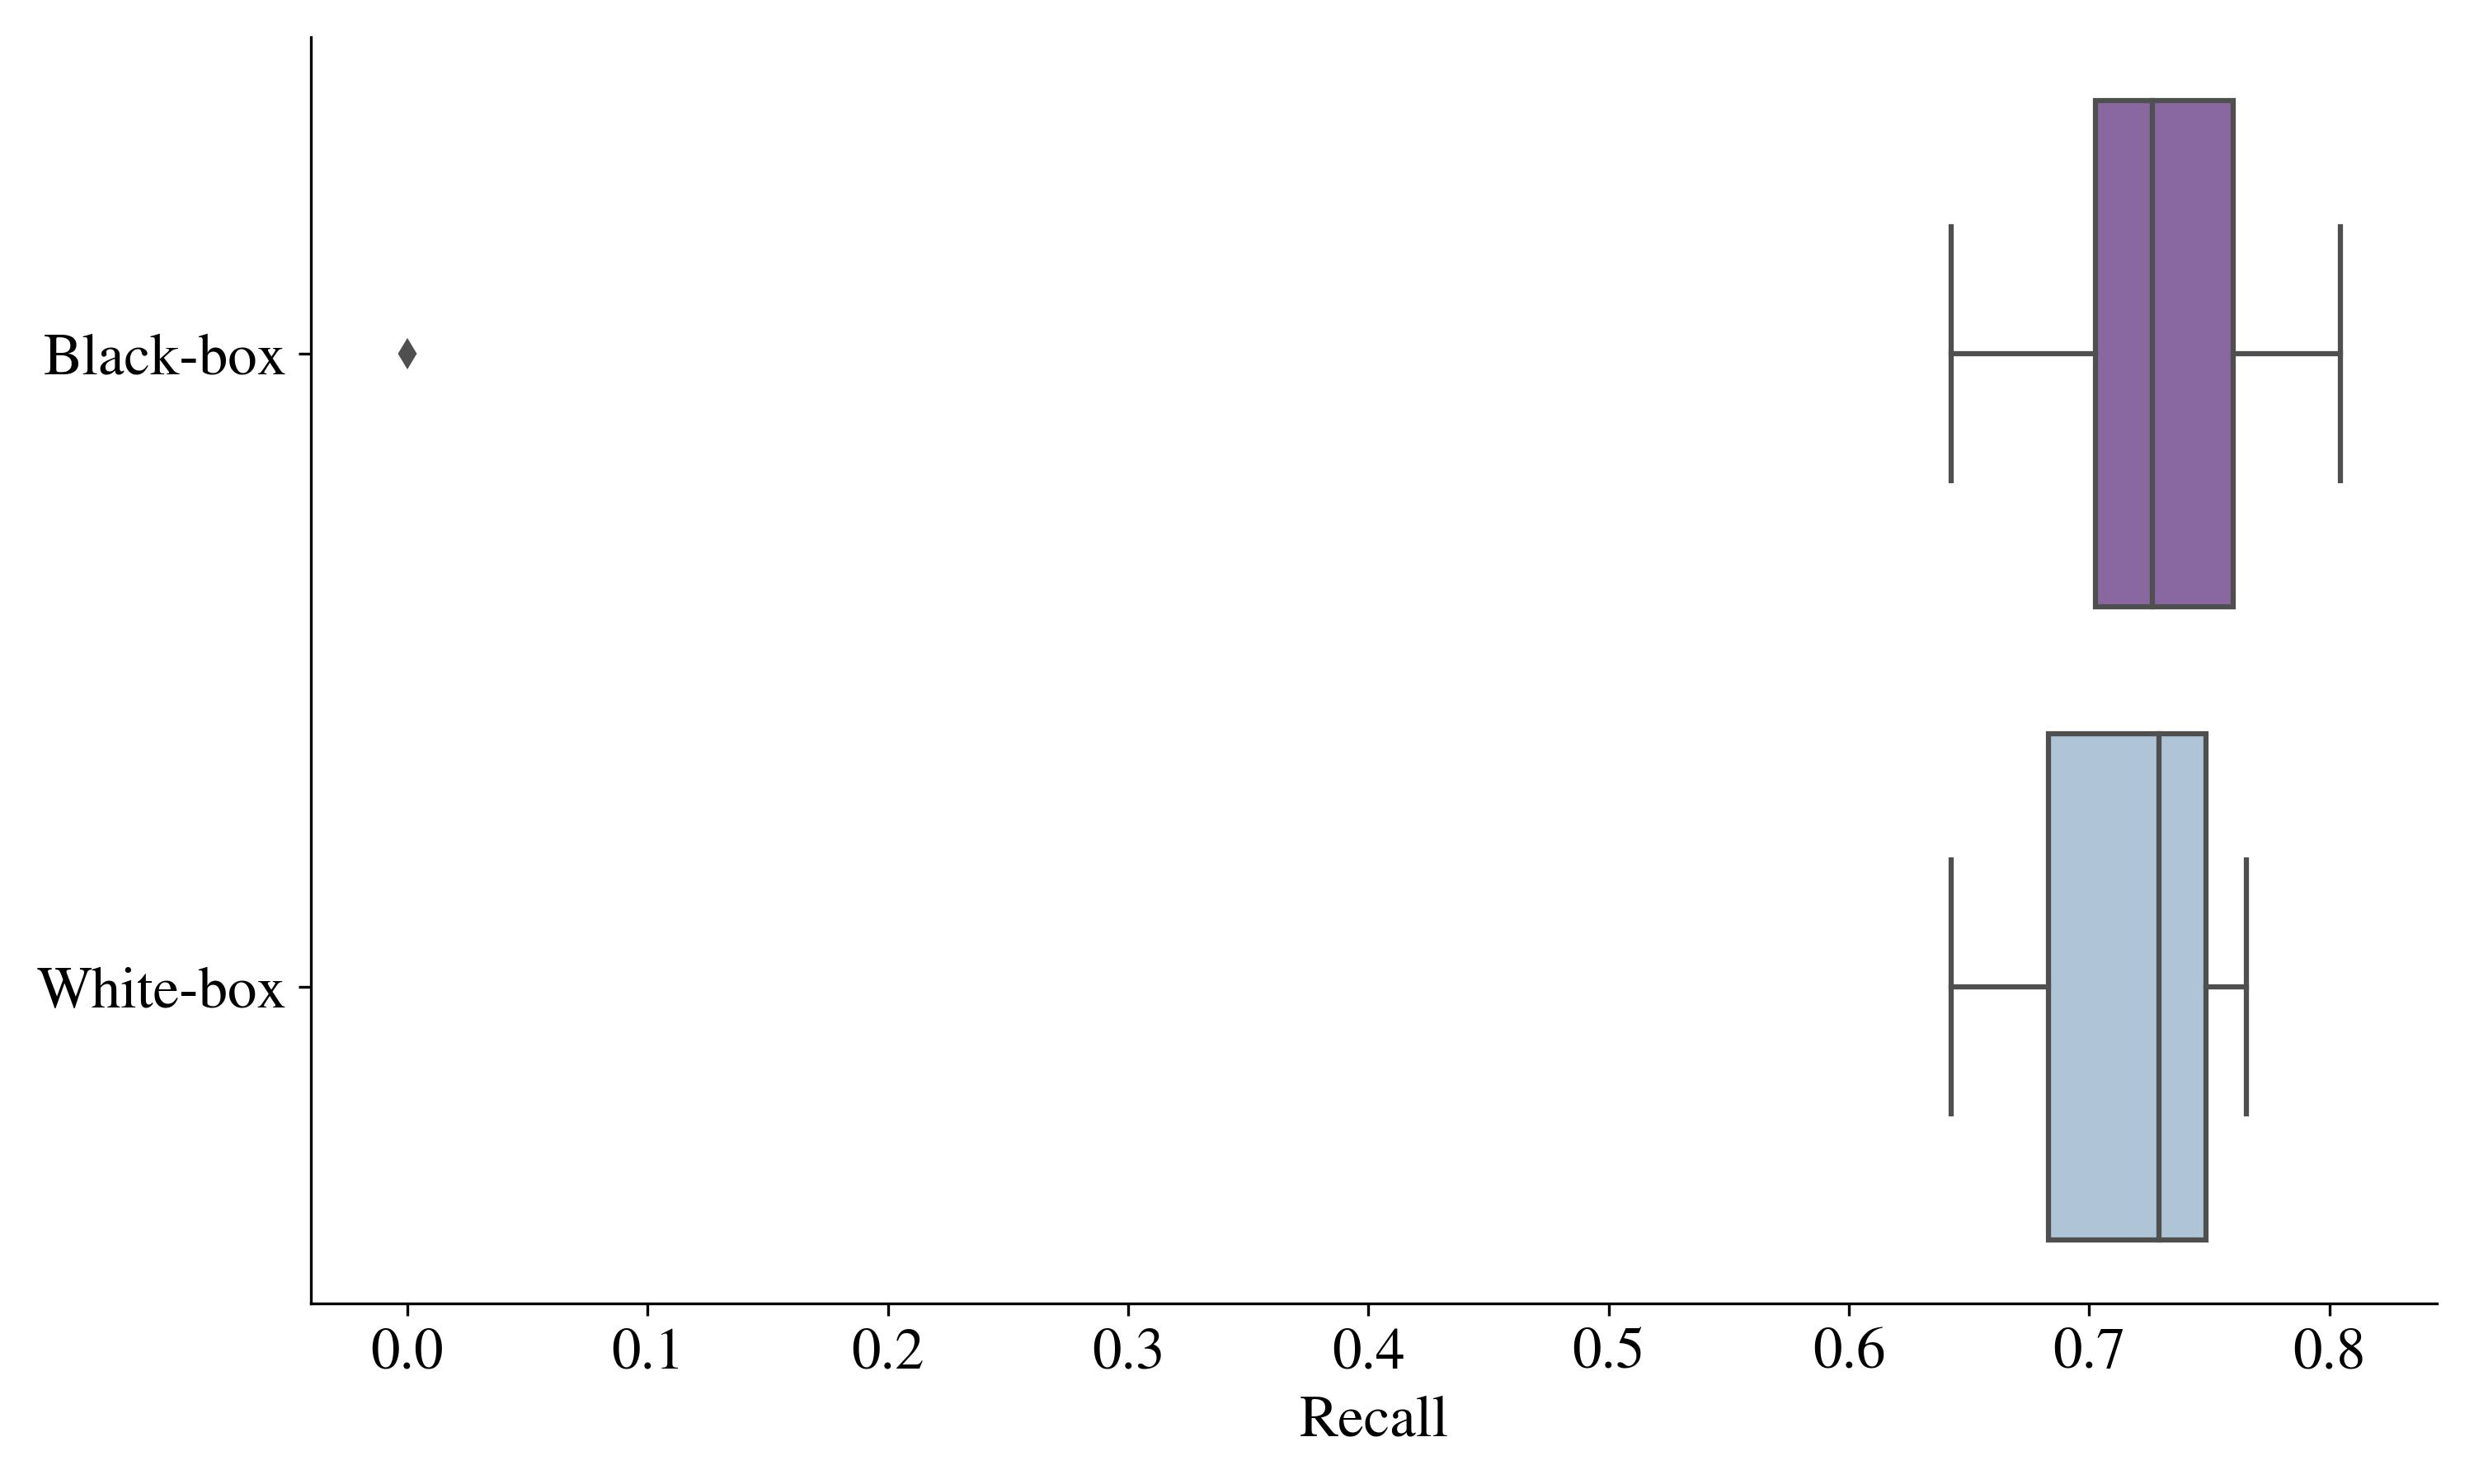
\includegraphics[width=140mm]{Figures/RECALL_Distribution_BB_WB.jpg}
    
    \centering{\begin{source}Author's results in Python\end{source}}\vspace{-1em}
\end{figure}

\begin{figure}[H]
    \centering
    \caption{Recall Distribution (Black--box/White--box dimension) - \textit{without outlier}}\vspace{0.5em}
    \label{fig:recdistwooutbbwb}
    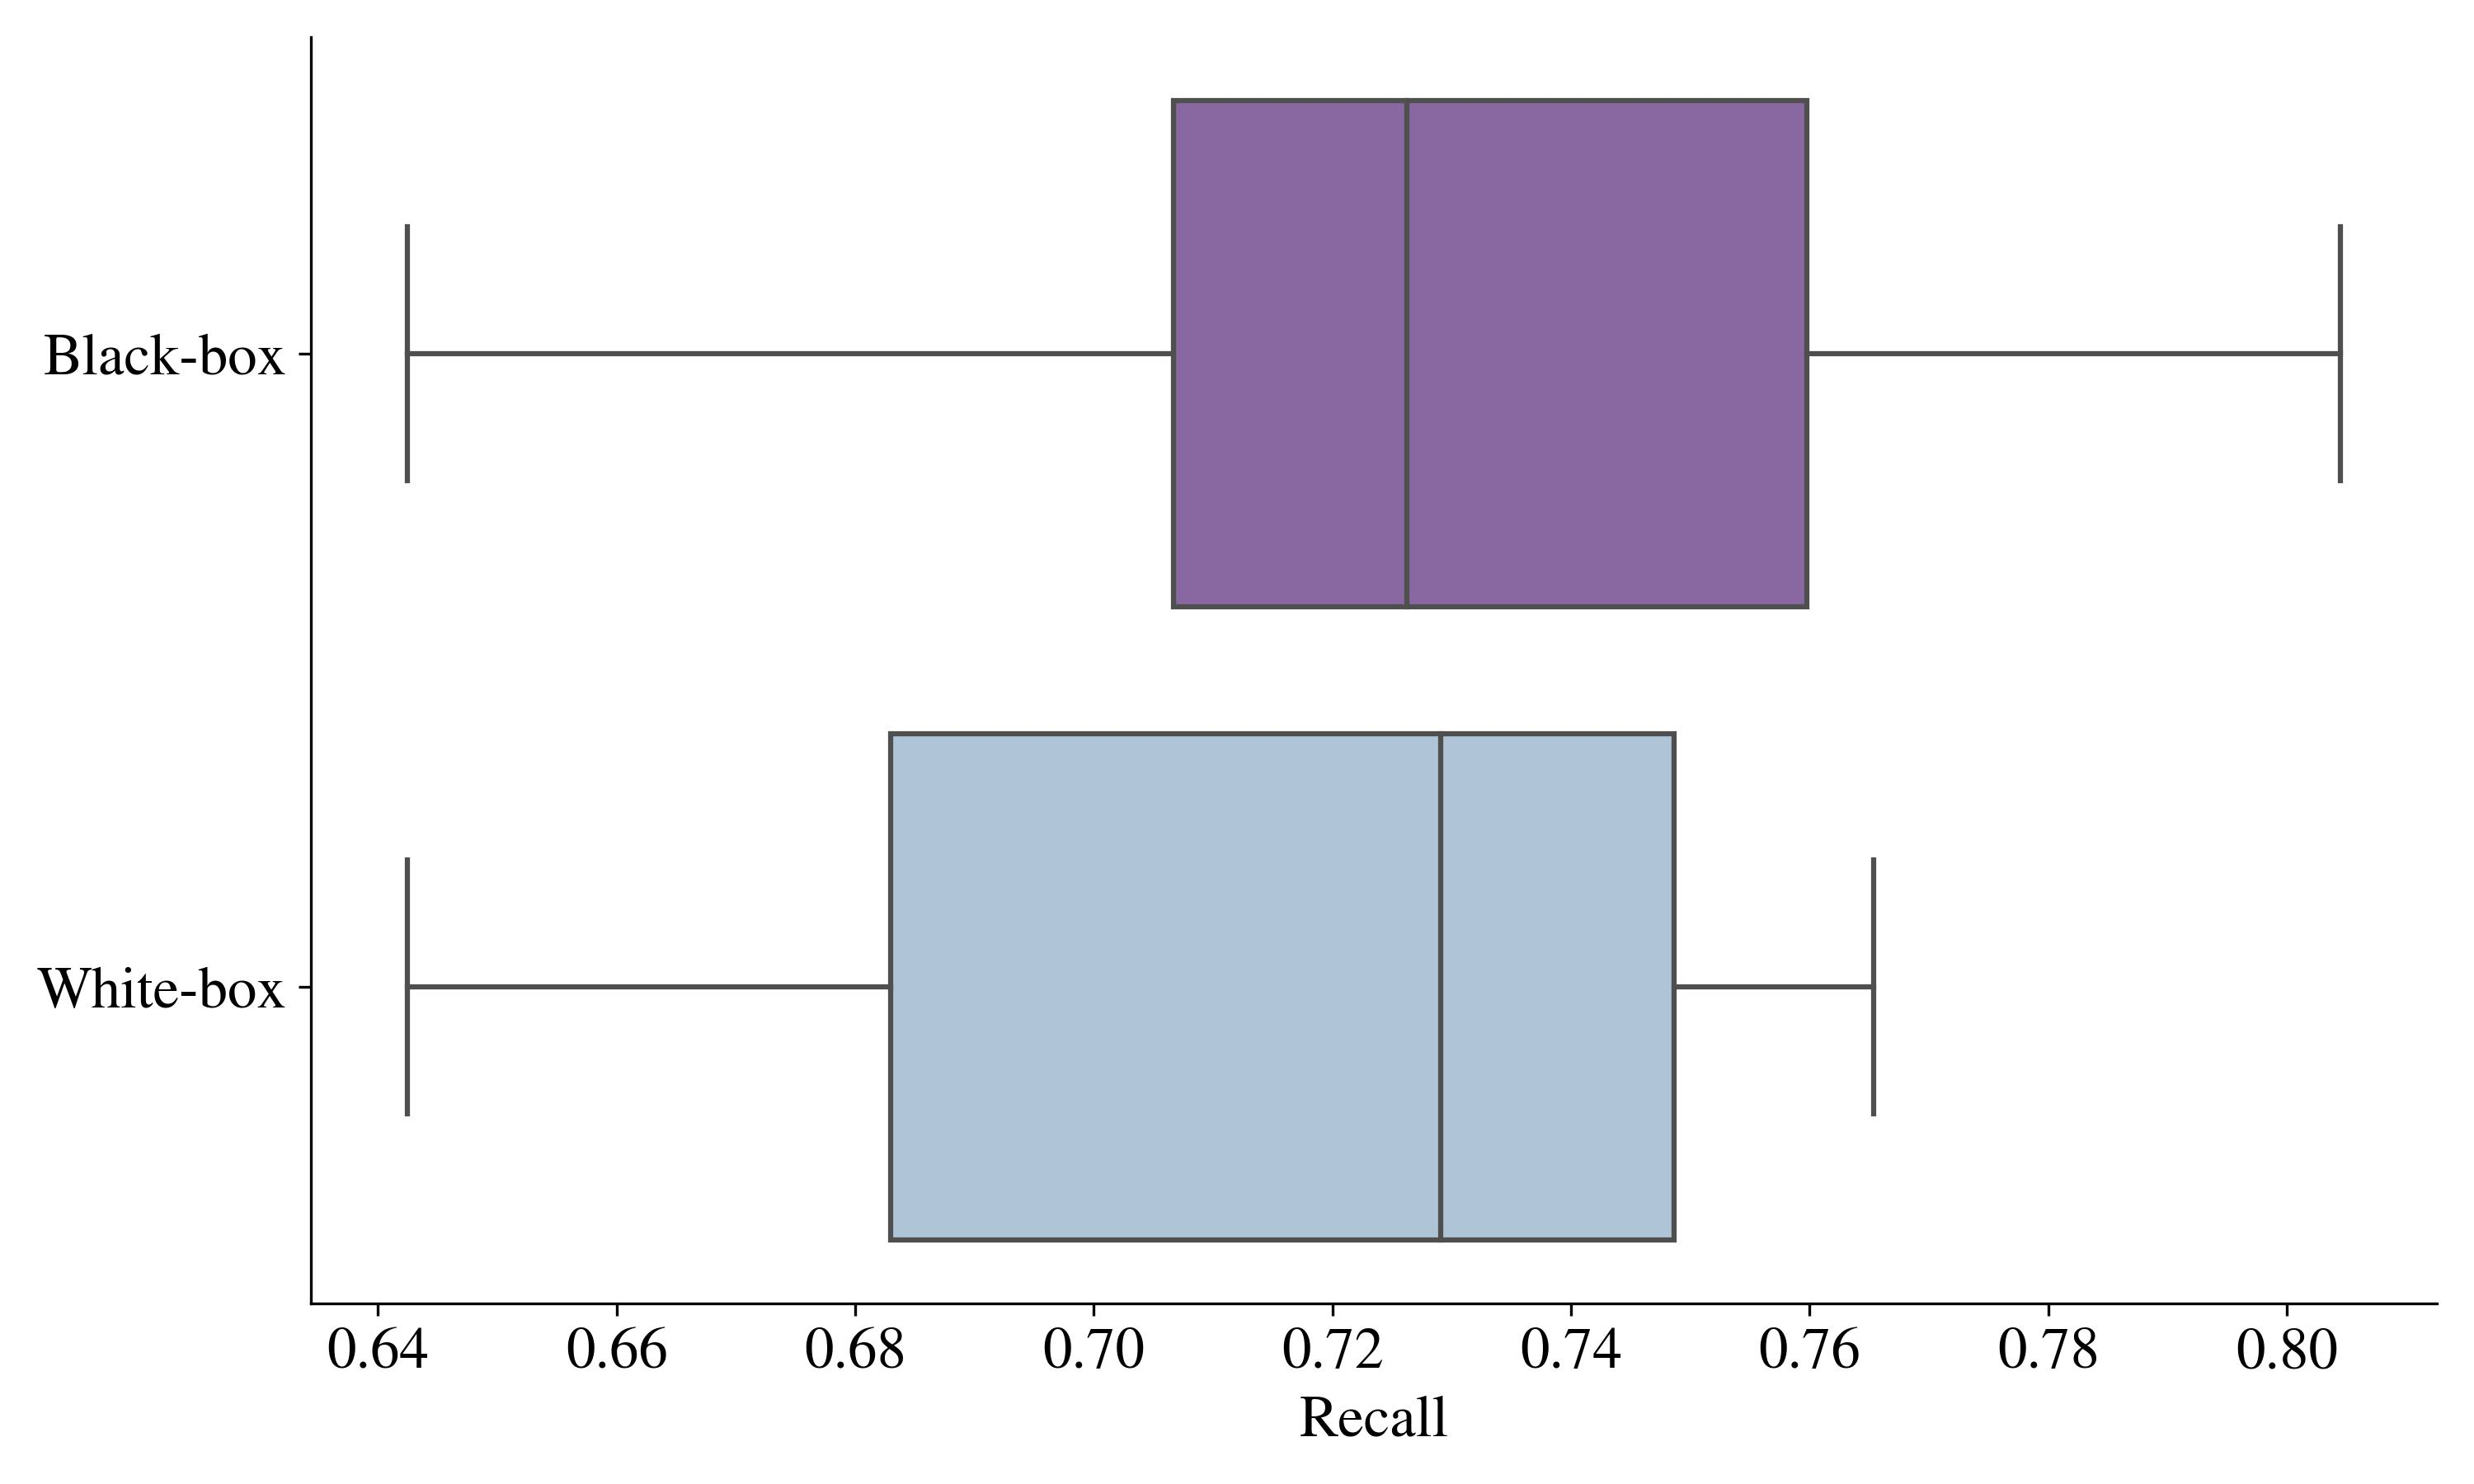
\includegraphics[width=140mm]{Figures/RECALL_WO_OUTLIERS_Distribution_BB_WB.jpg}
    
    \centering{\begin{source}Author's results in Python\end{source}}\vspace{-1em}
\end{figure}

\begin{figure}[H]
    \centering
    \caption{Accuracy Distribution}\vspace{0.5em}
    \label{fig:accdist}
    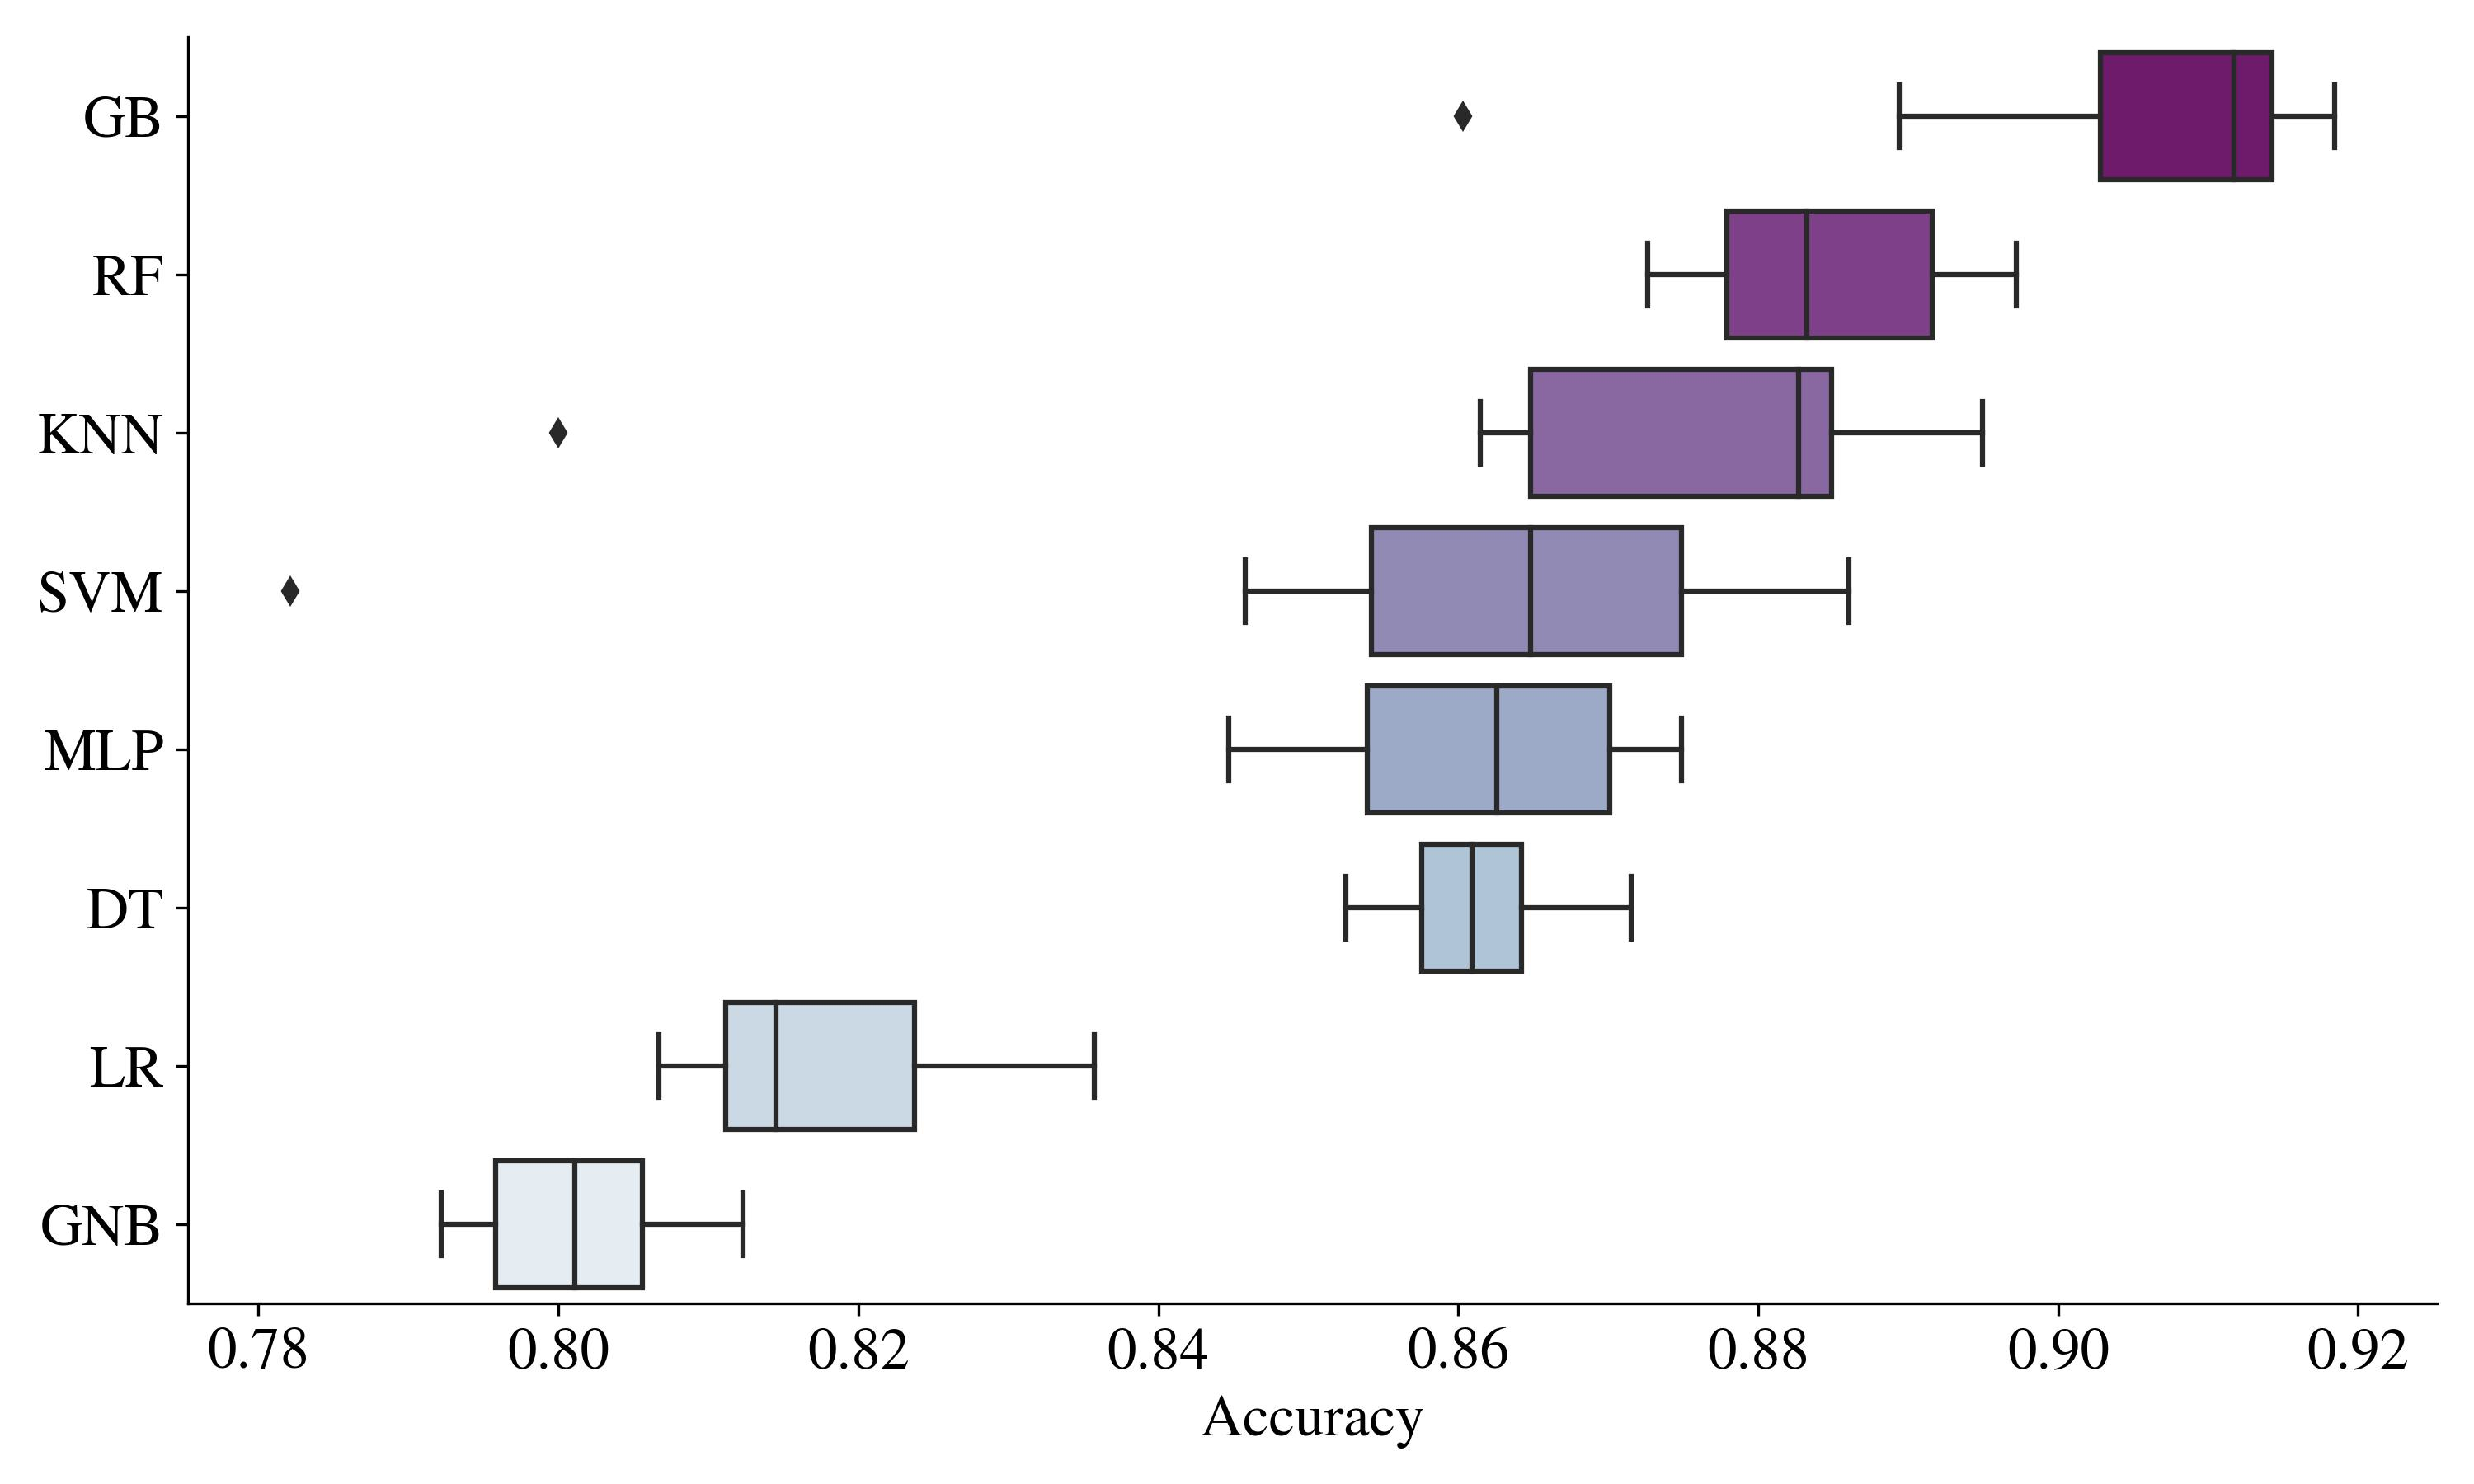
\includegraphics[width=140mm]{Figures/ACCURACY_Distribution.jpg}
    
    \centering{\begin{source}Author's results in Python\end{source}}\vspace{-1em}
\end{figure}

\begin{figure}[H]
    \centering
    \caption{Accuracy Distribution (Black--box/White--box dimension)}\vspace{0.5em}
    \label{fig:accdistbbwb}
    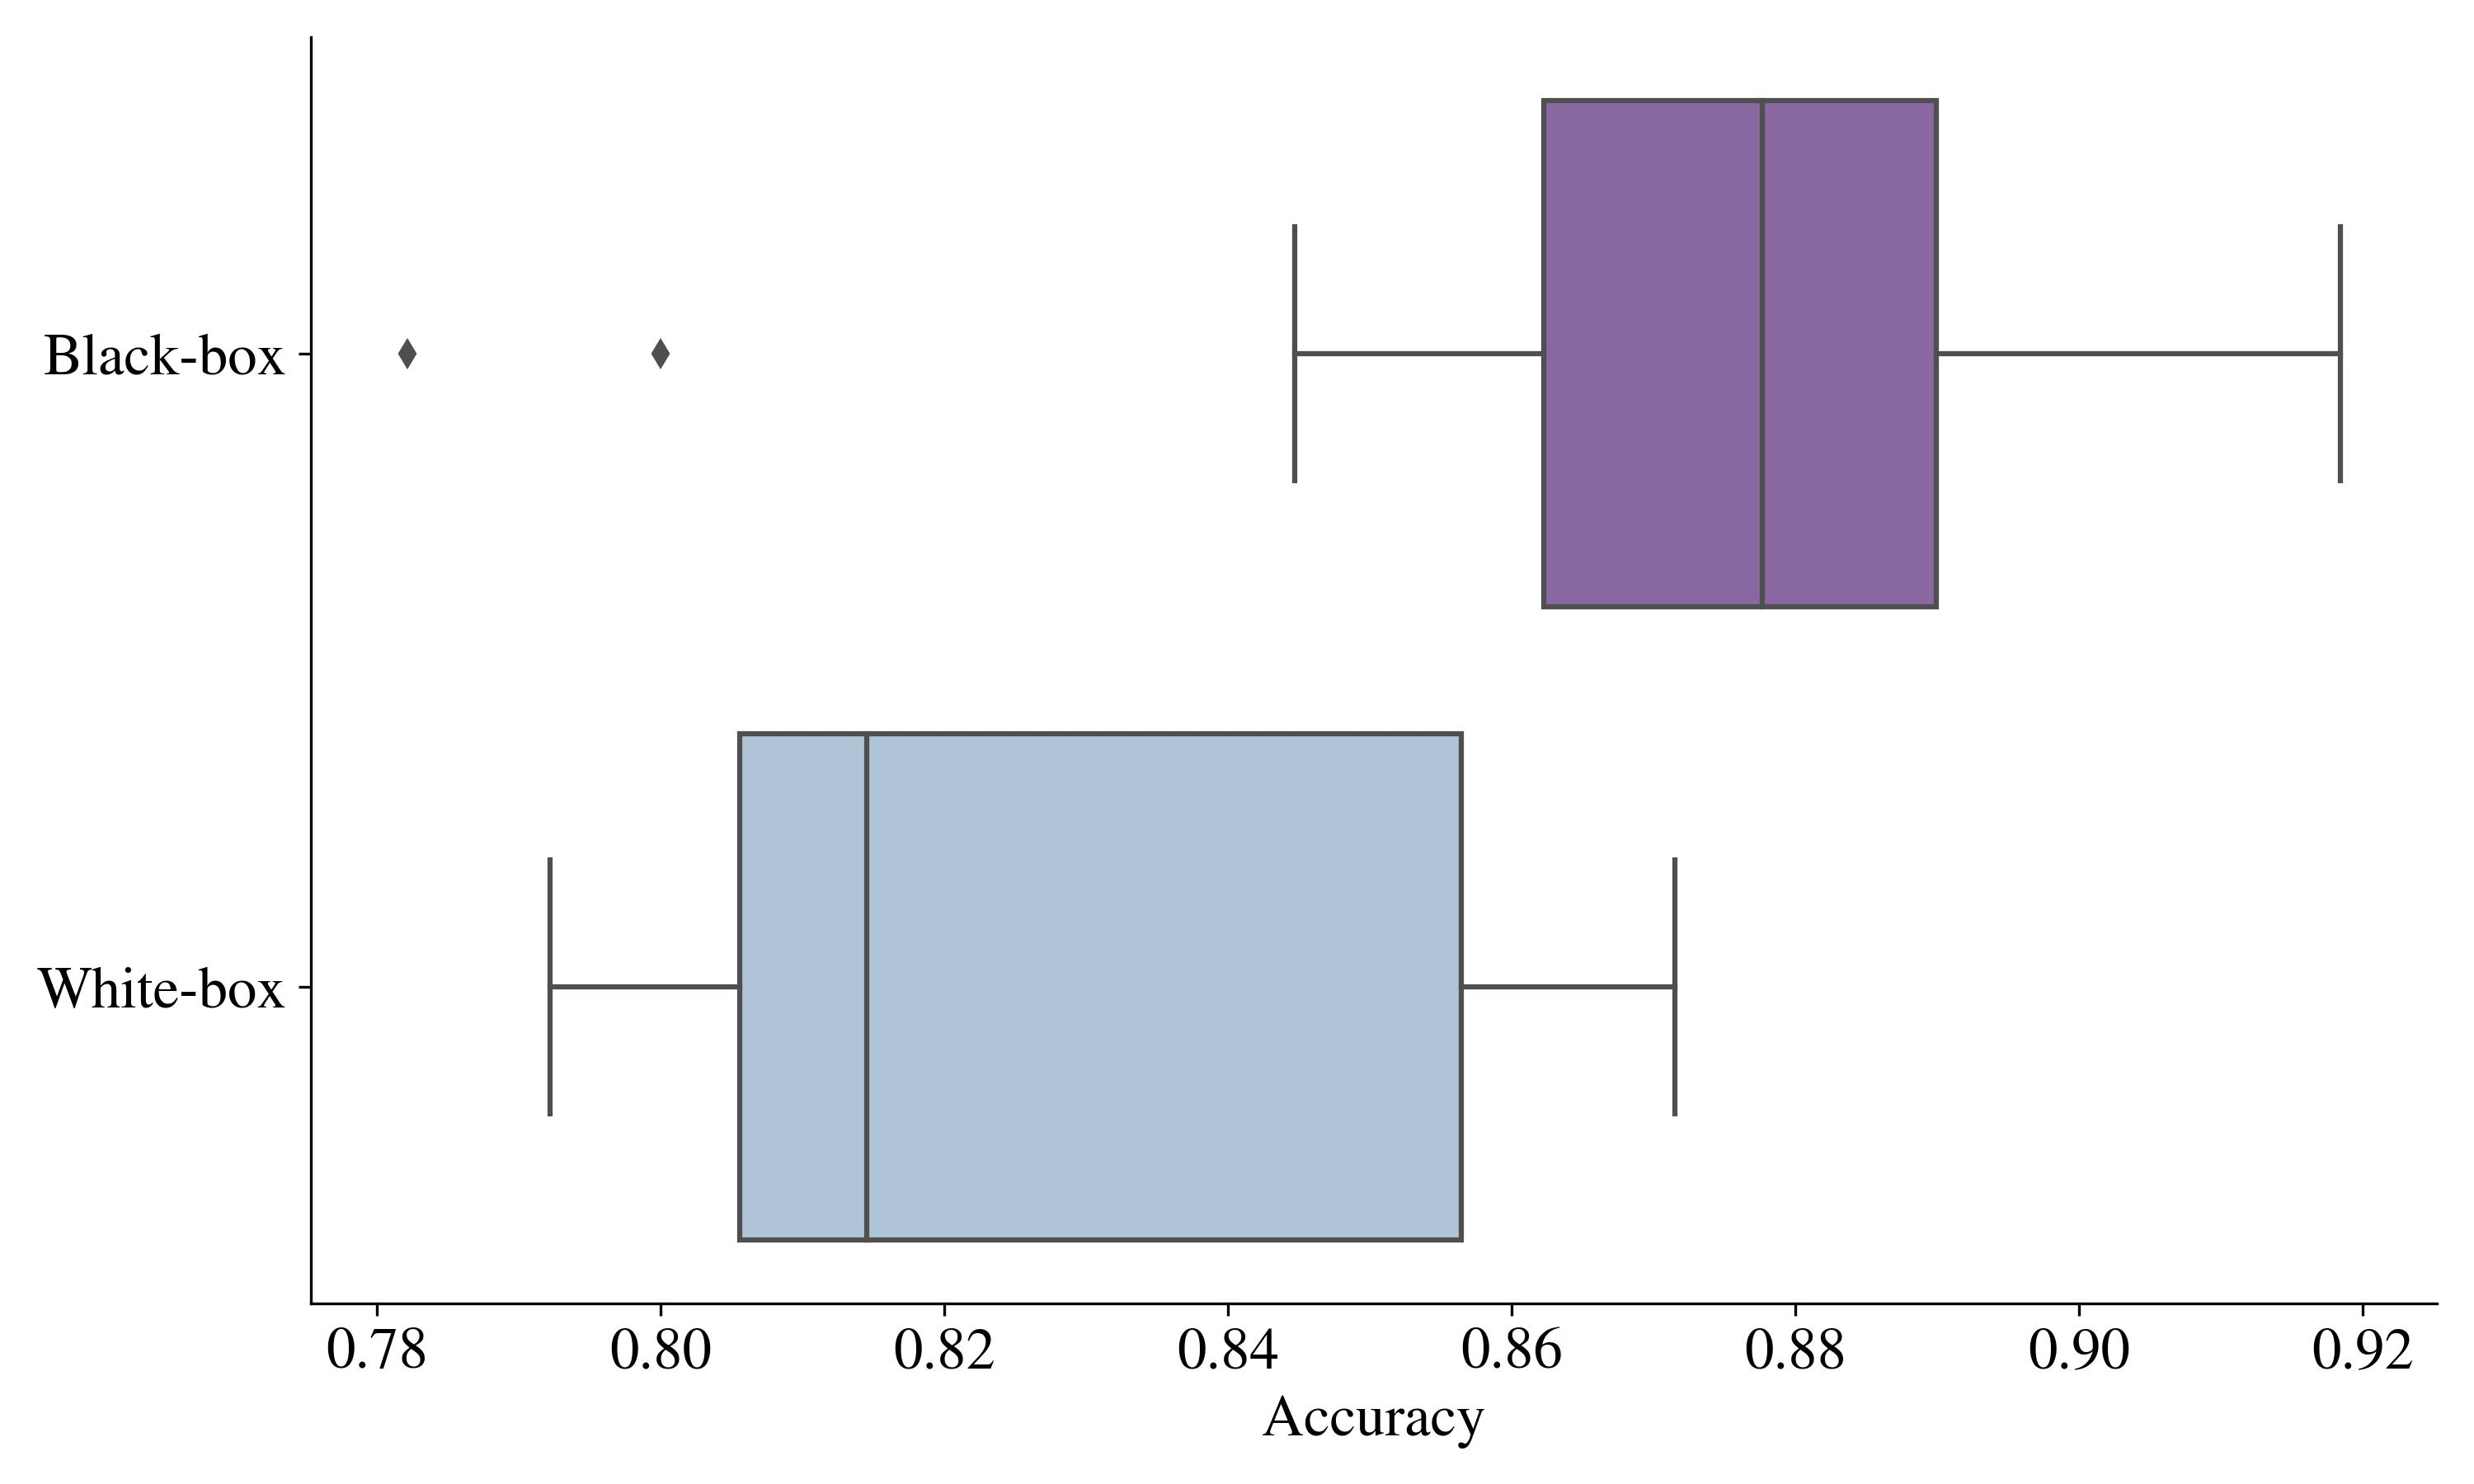
\includegraphics[width=140mm]{Figures/ACCURACY_Distribution_BB_WB.jpg}
    
    \centering{\begin{source}Author's results in Python\end{source}}\vspace{-1em}
\end{figure}

\begin{figure}[H]
    \centering
    \caption{AUC Distribution}\vspace{0.5em}
    \label{fig:aucdist}
    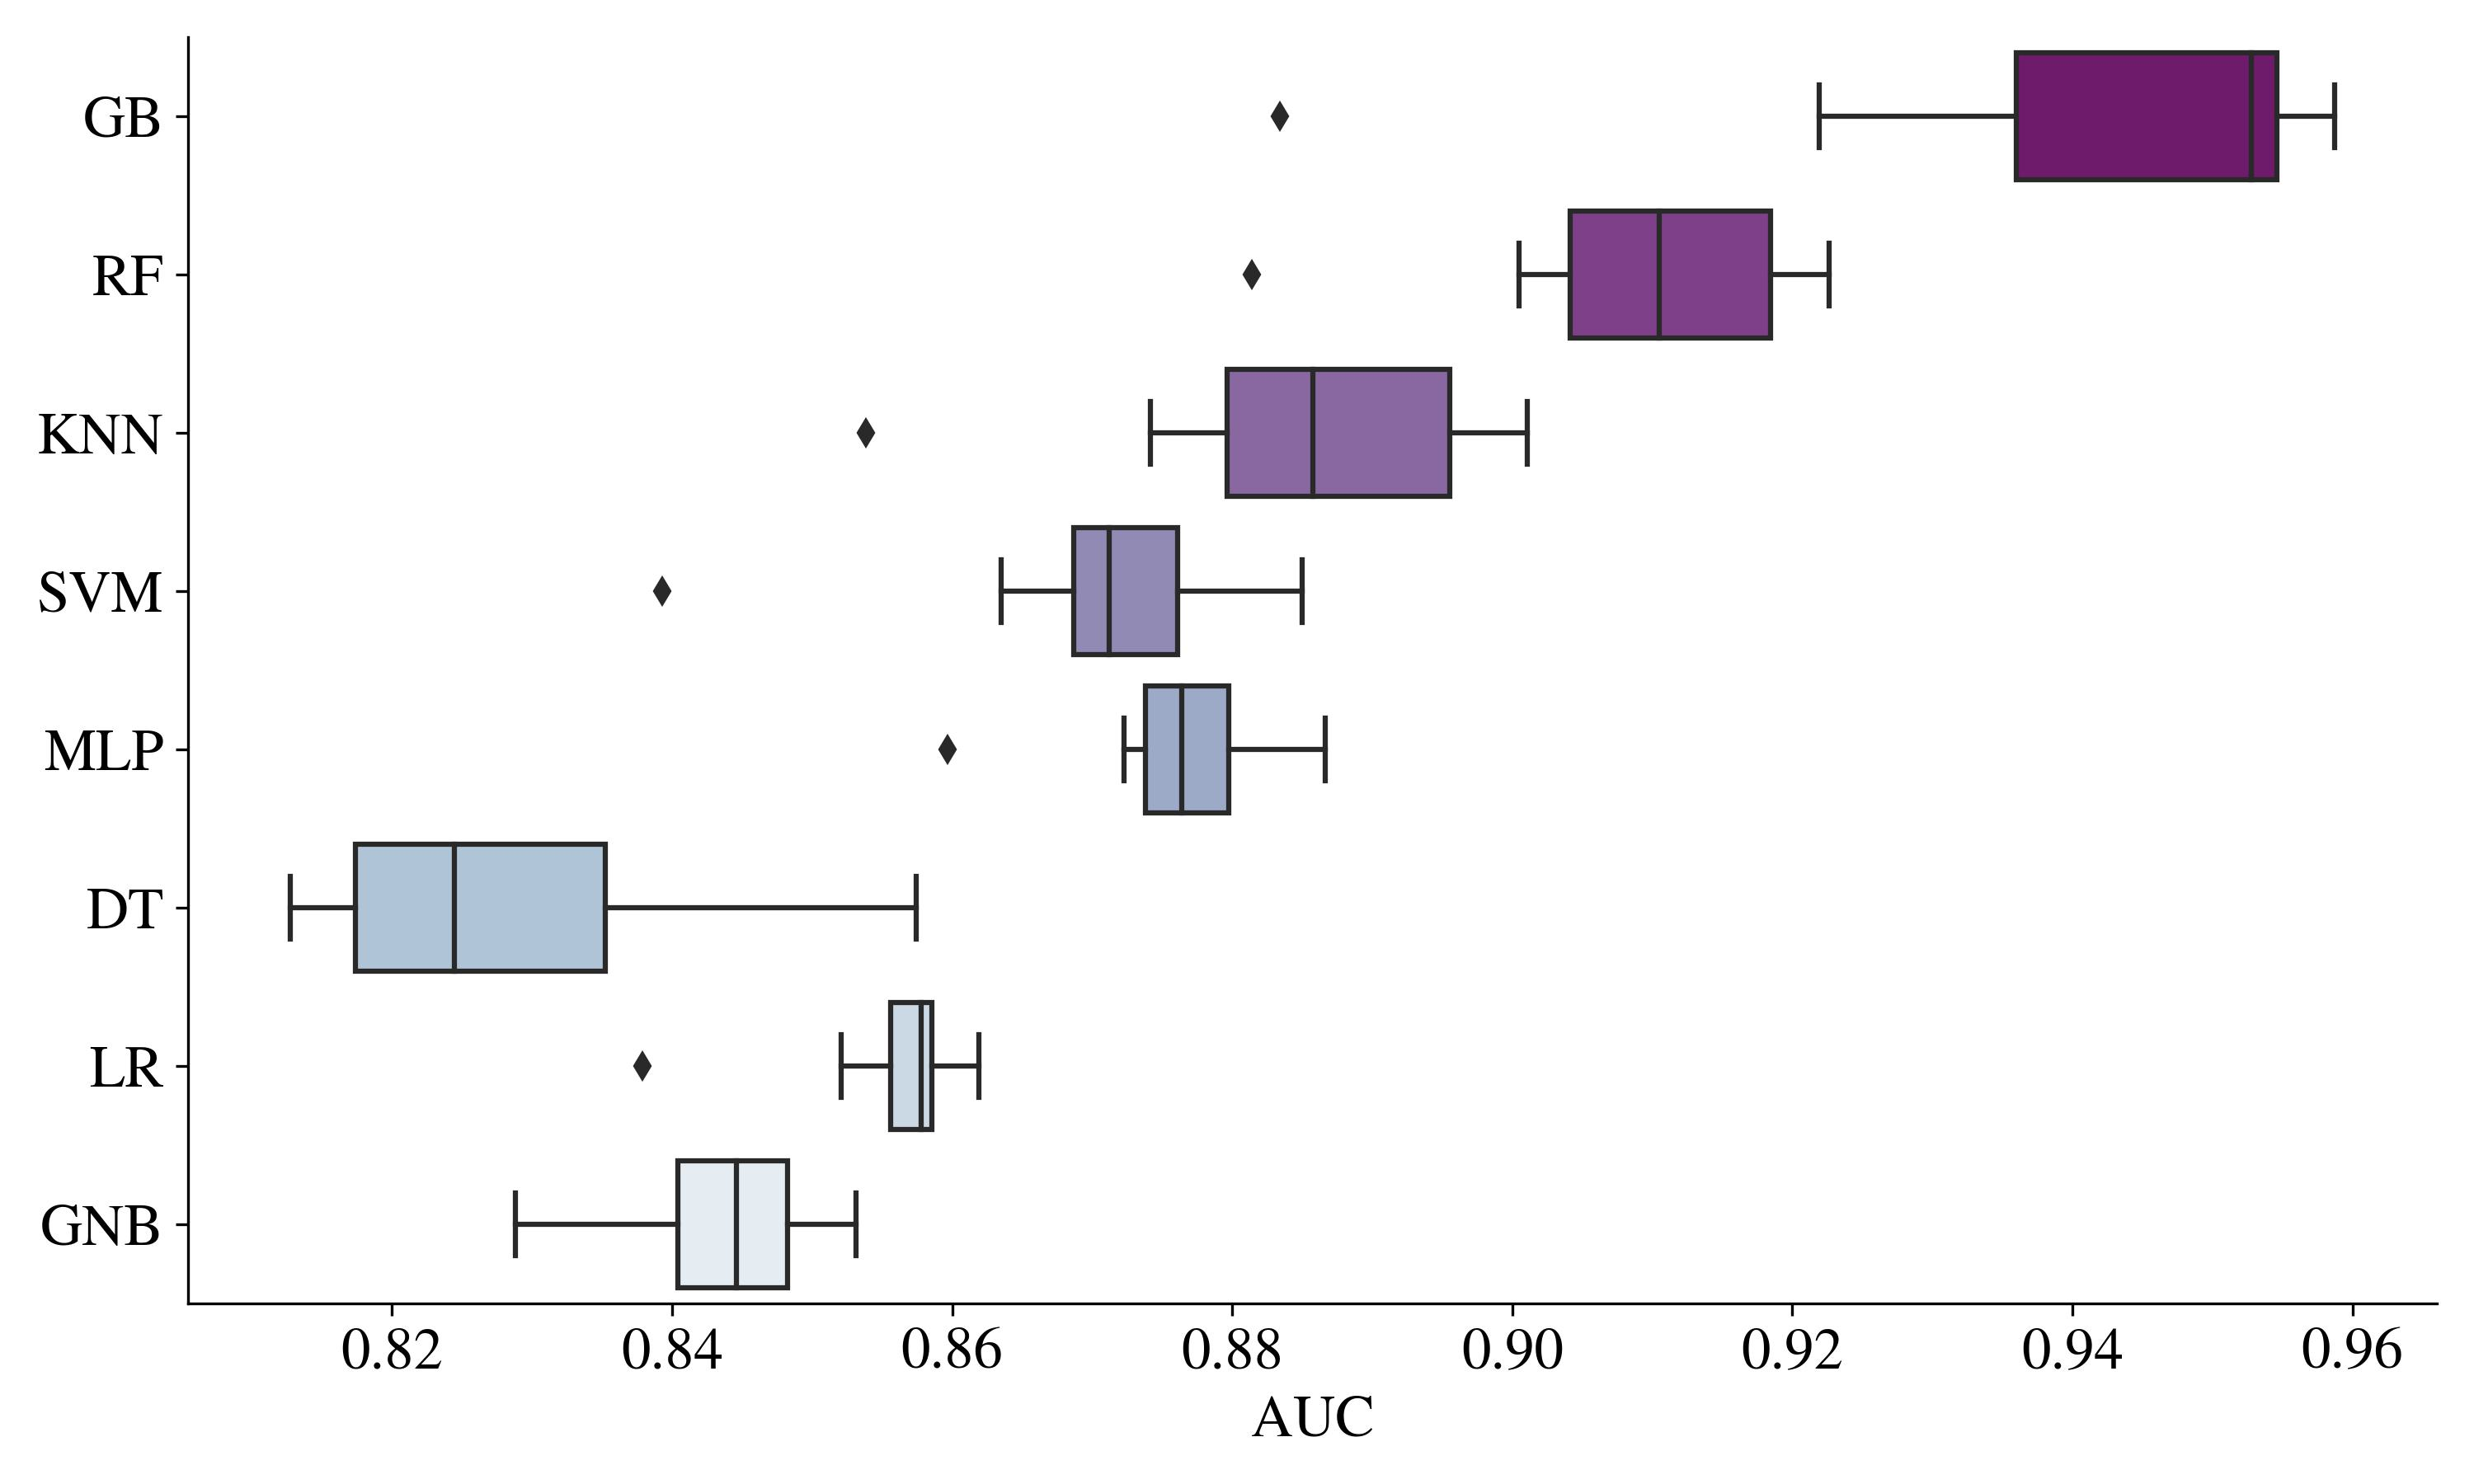
\includegraphics[width=140mm]{Figures/AUC_Distribution.jpg}
    
    \centering{\begin{source}Author's results in Python\end{source}}\vspace{-1em}
\end{figure}

\begin{figure}[H]
    \centering
    \caption{AUC Distribution (Black--box/White--box dimension)}\vspace{0.5em}
    \label{fig:aucdistbbwb}
    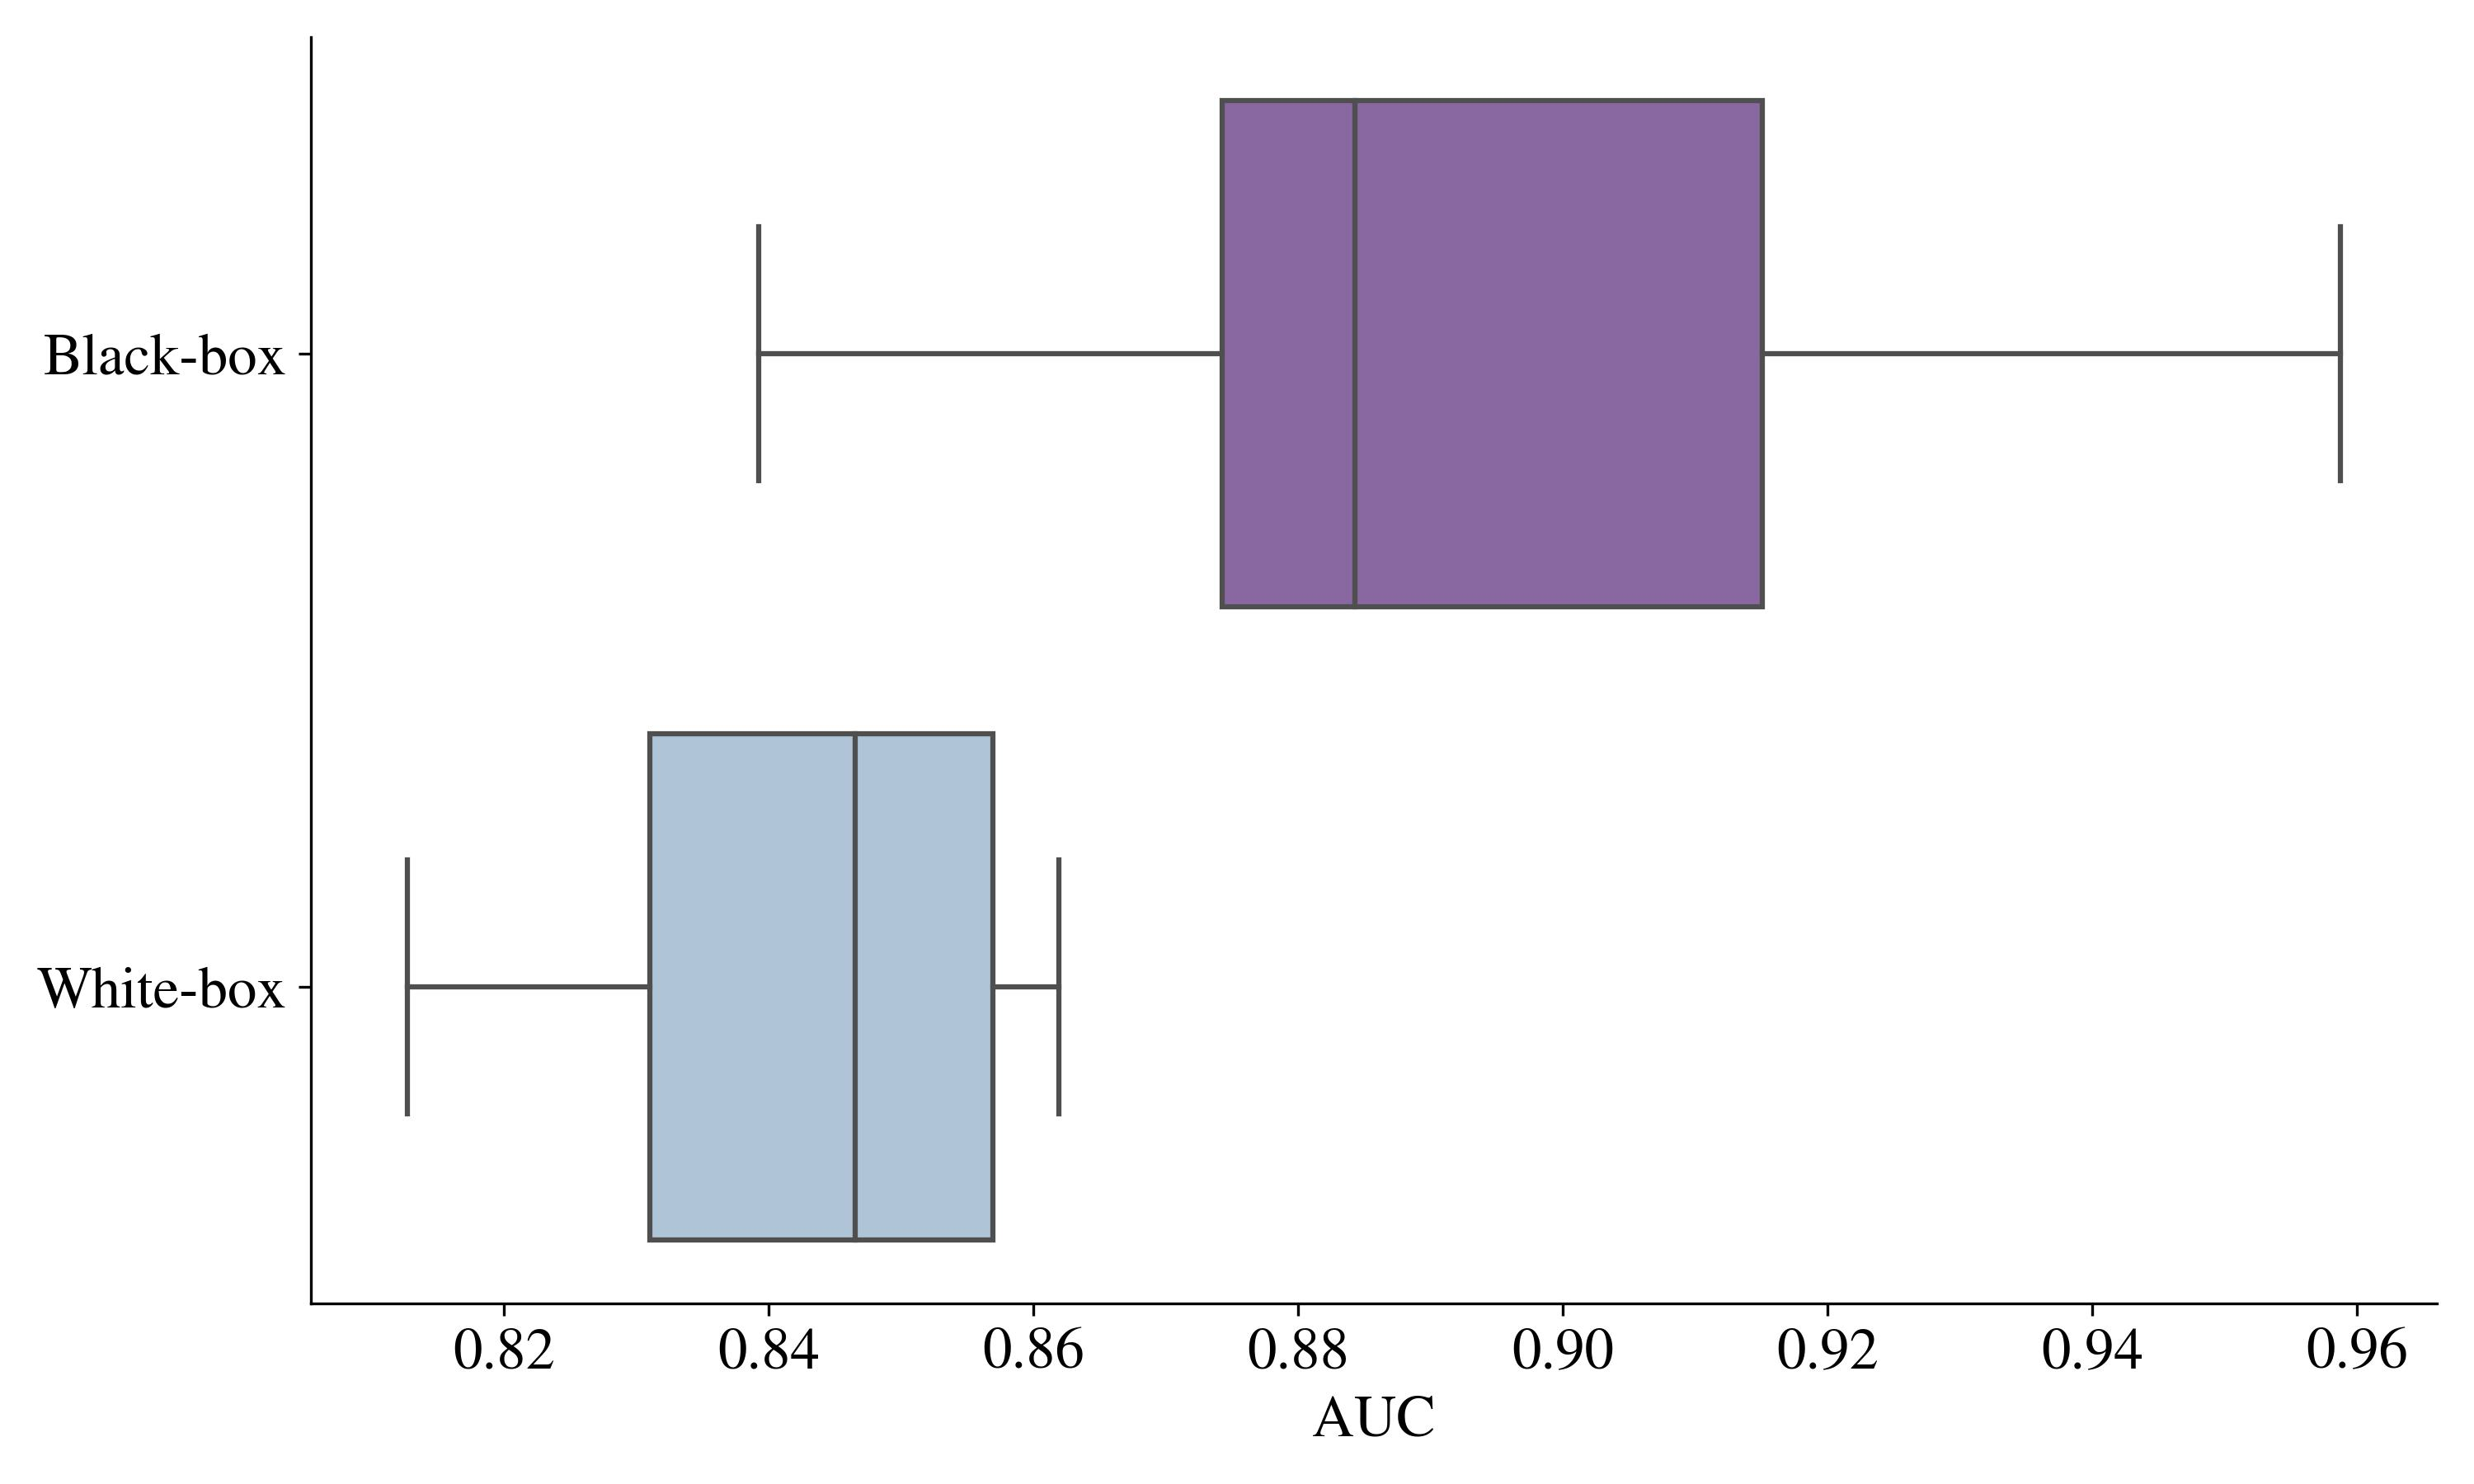
\includegraphics[width=140mm]{Figures/AUC_Distribution_BB_WB.jpg}
    
    \centering{\begin{source}Author's results in Python\end{source}}\vspace{-1em}
\end{figure}

\begin{figure}[H]
    \centering
    \caption{Matthews Correlation Coefficient Distribution}\vspace{0.5em}
    \label{fig:mccdist}
    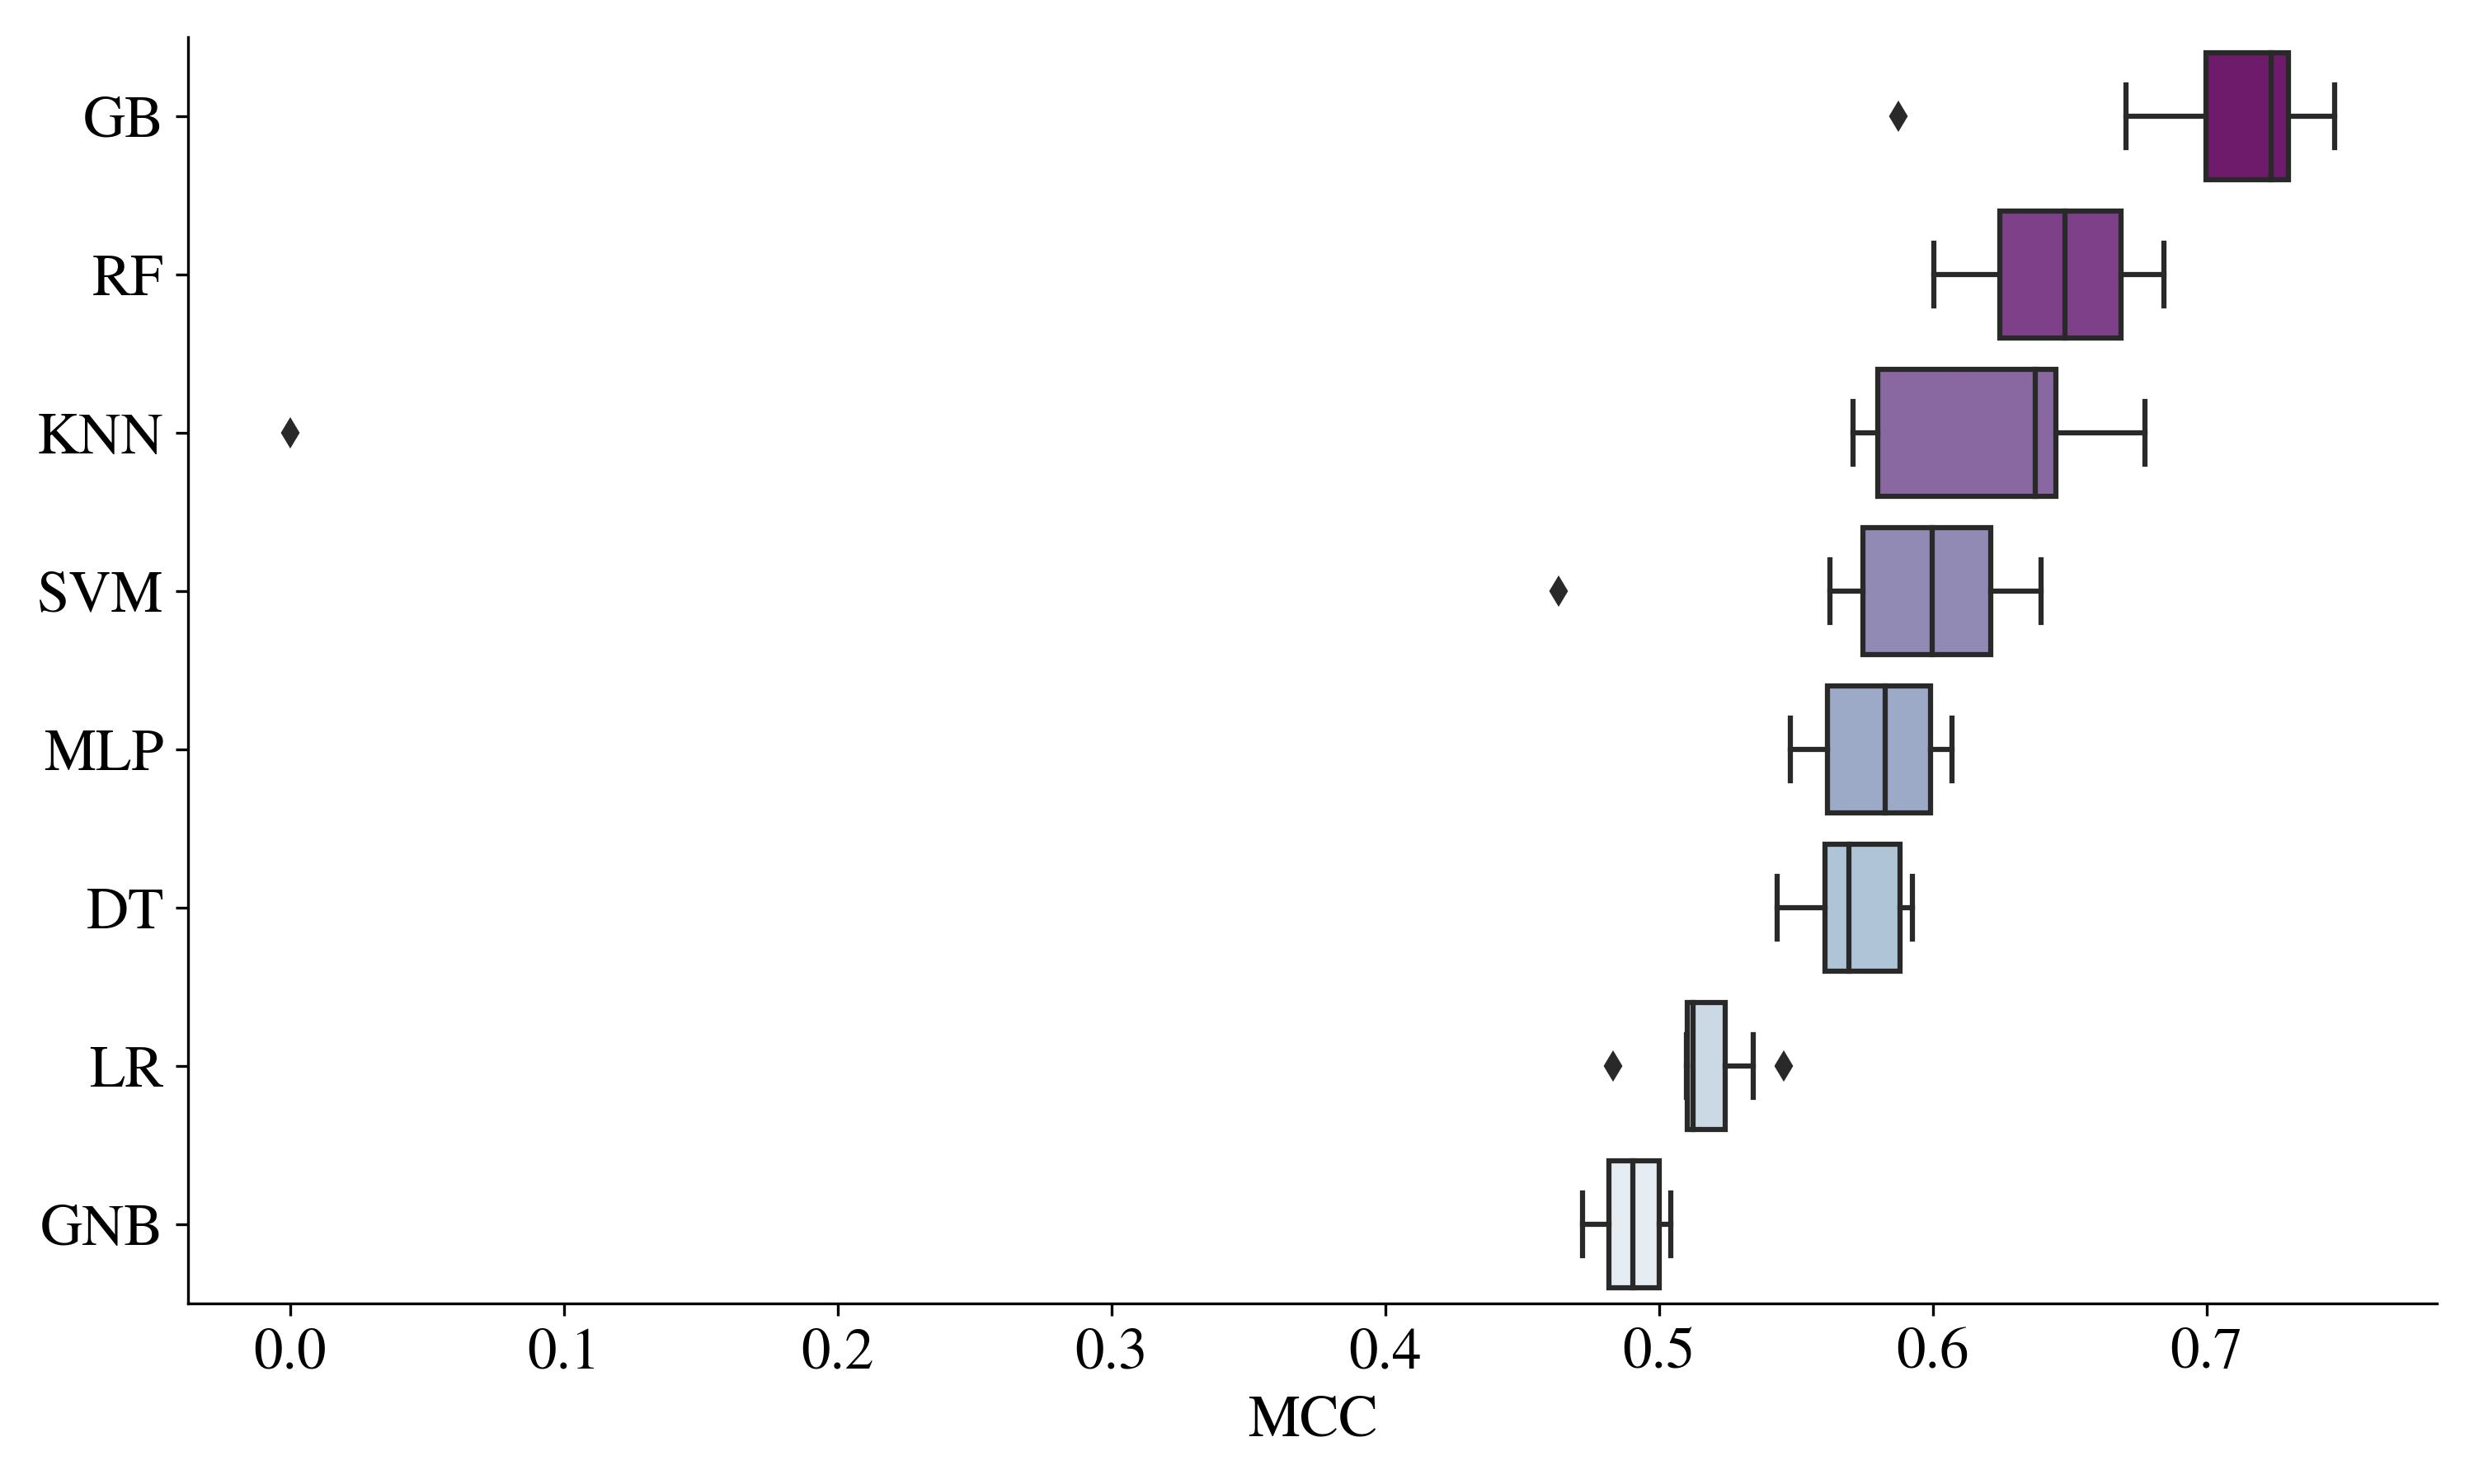
\includegraphics[width=140mm]{Figures/MCC_Distribution.jpg}
    
    \centering{\begin{source}Author's results in Python\end{source}}\vspace{-1em}
\end{figure}

\begin{figure}[H]
    \centering
    \caption{Matthews Correlation Coefficient Distribution - \textit{without outlier}}\vspace{0.5em}
    \label{fig:mccdistwoout}
    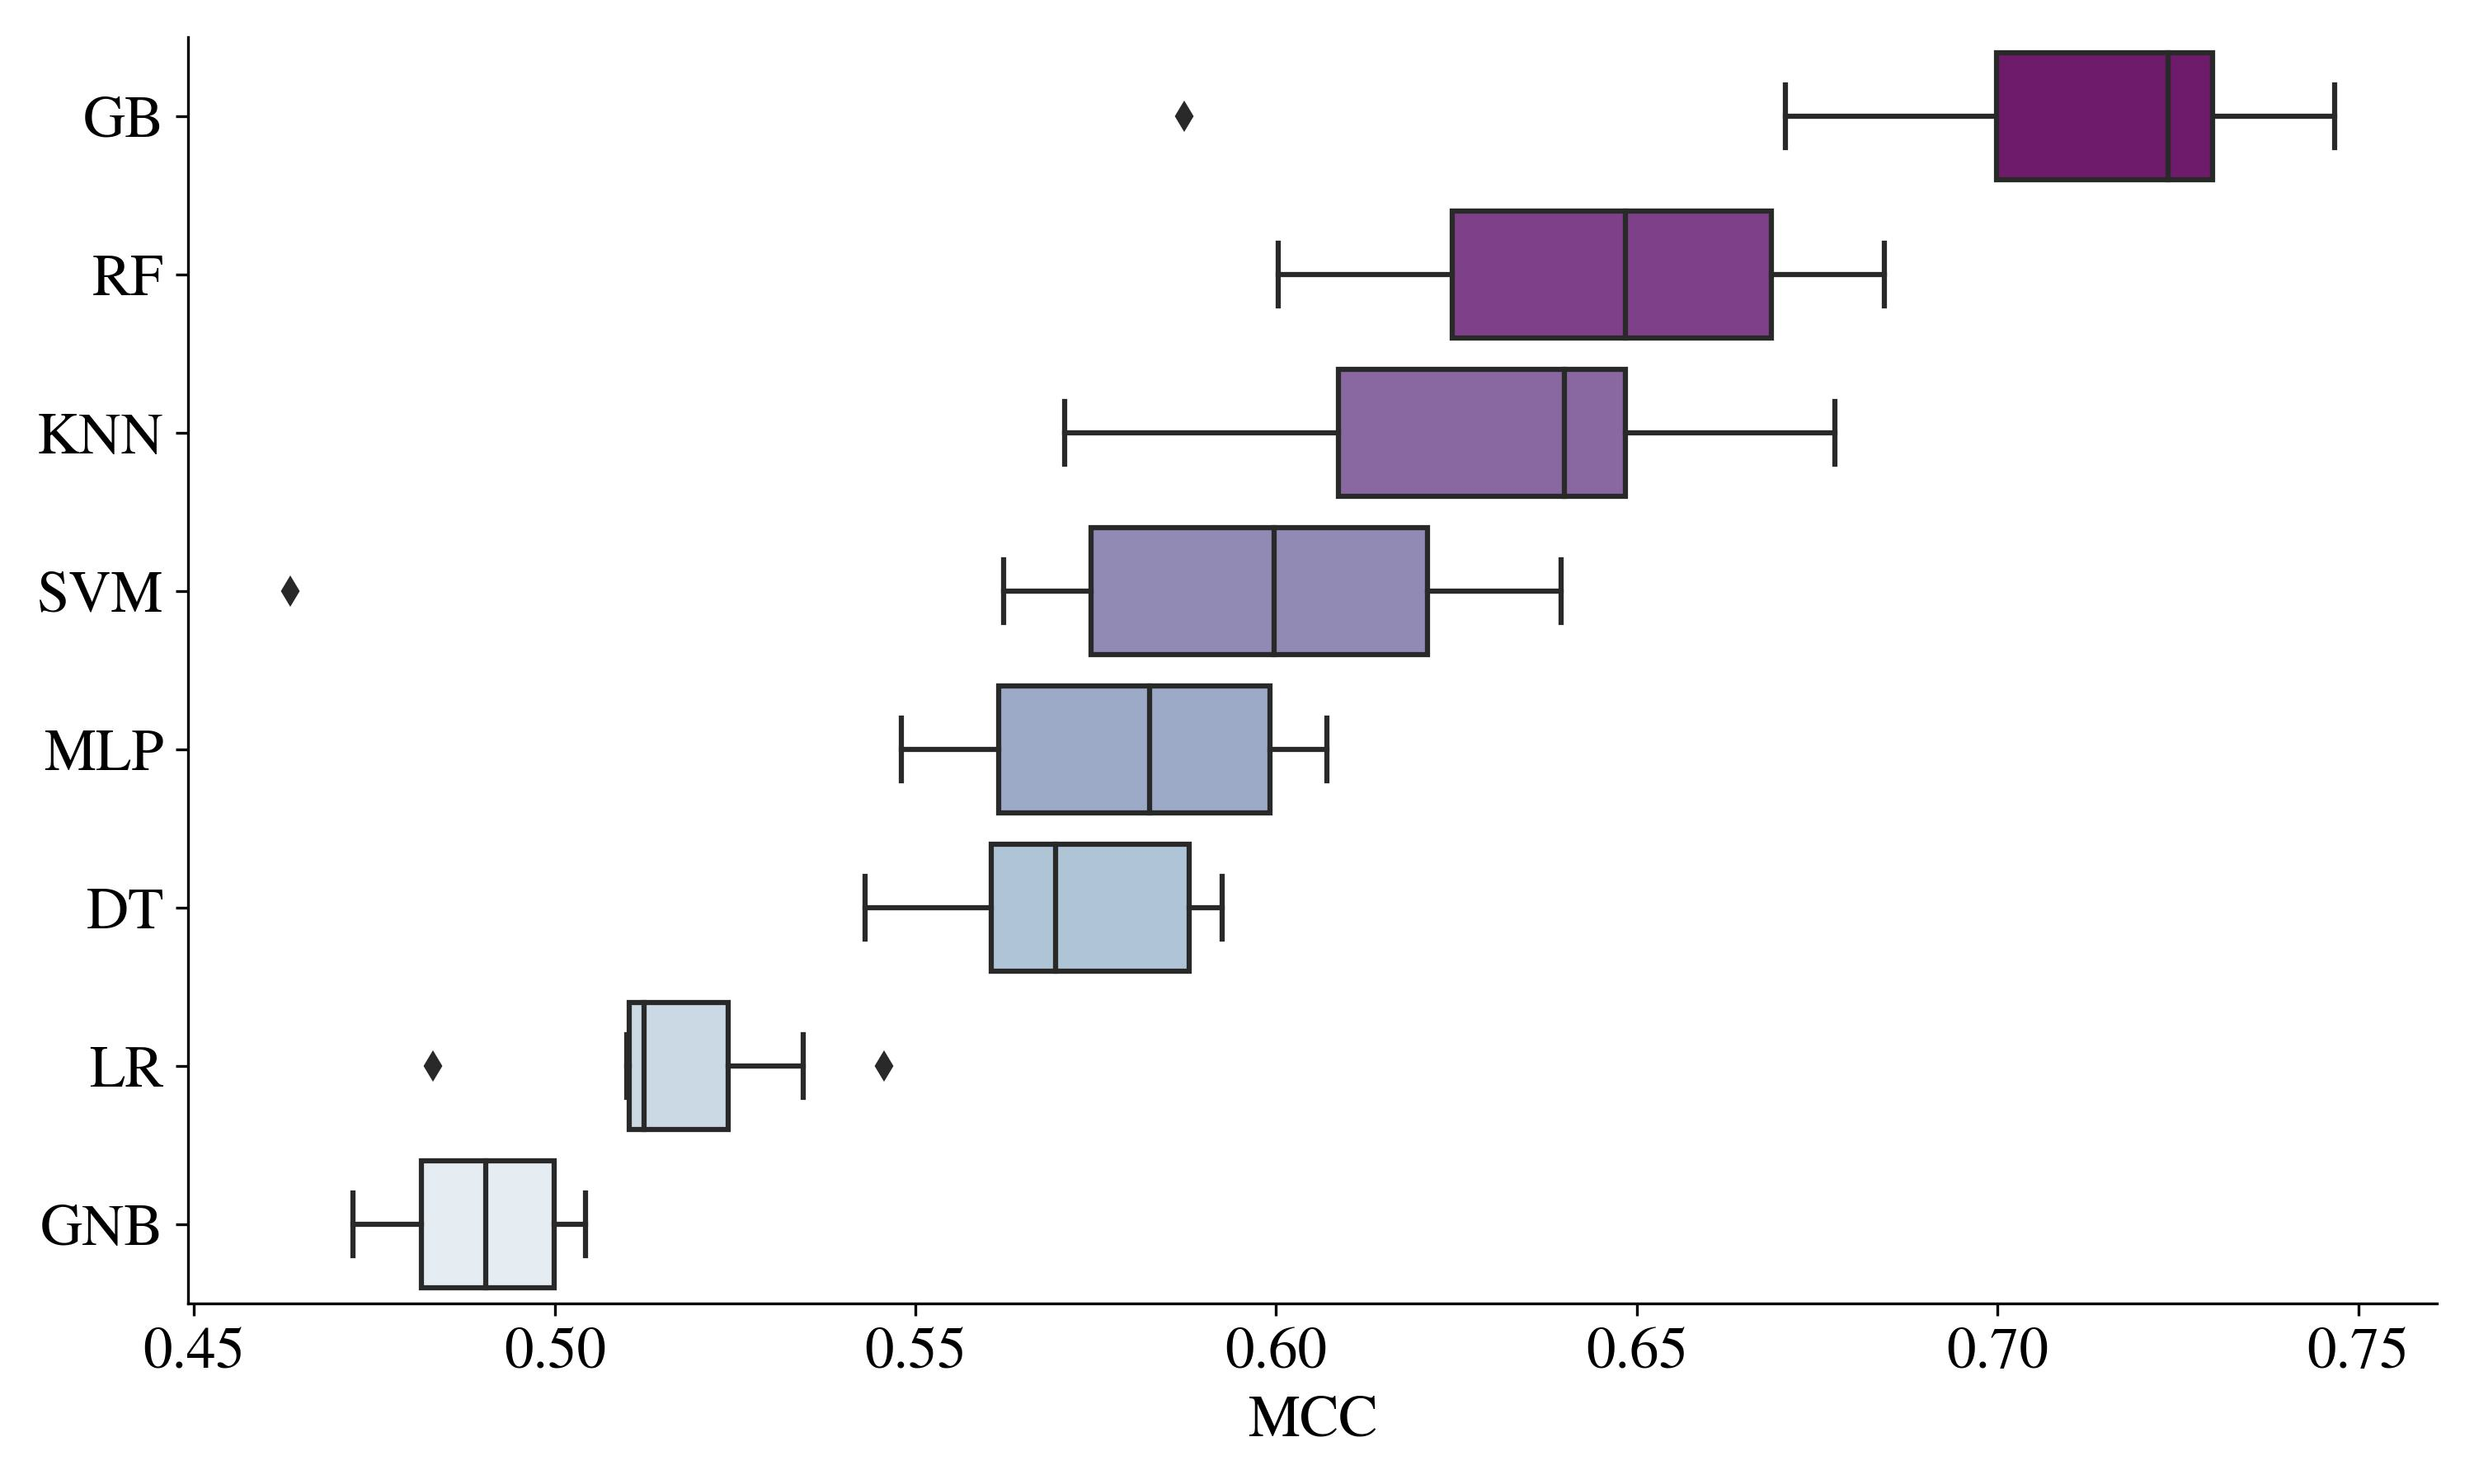
\includegraphics[width=140mm]{Figures/MCC_WO_OUTLIERS_Distribution.jpg}
    
    \centering{\begin{source}Author's results in Python\end{source}}\vspace{-1em}
\end{figure}

\begin{figure}[H]
    \centering
    \caption{Matthews Correlation Coefficient Distribution (Black--box/White--box dimension)}\vspace{0.5em}
    \label{fig:mccdistbbwb}
    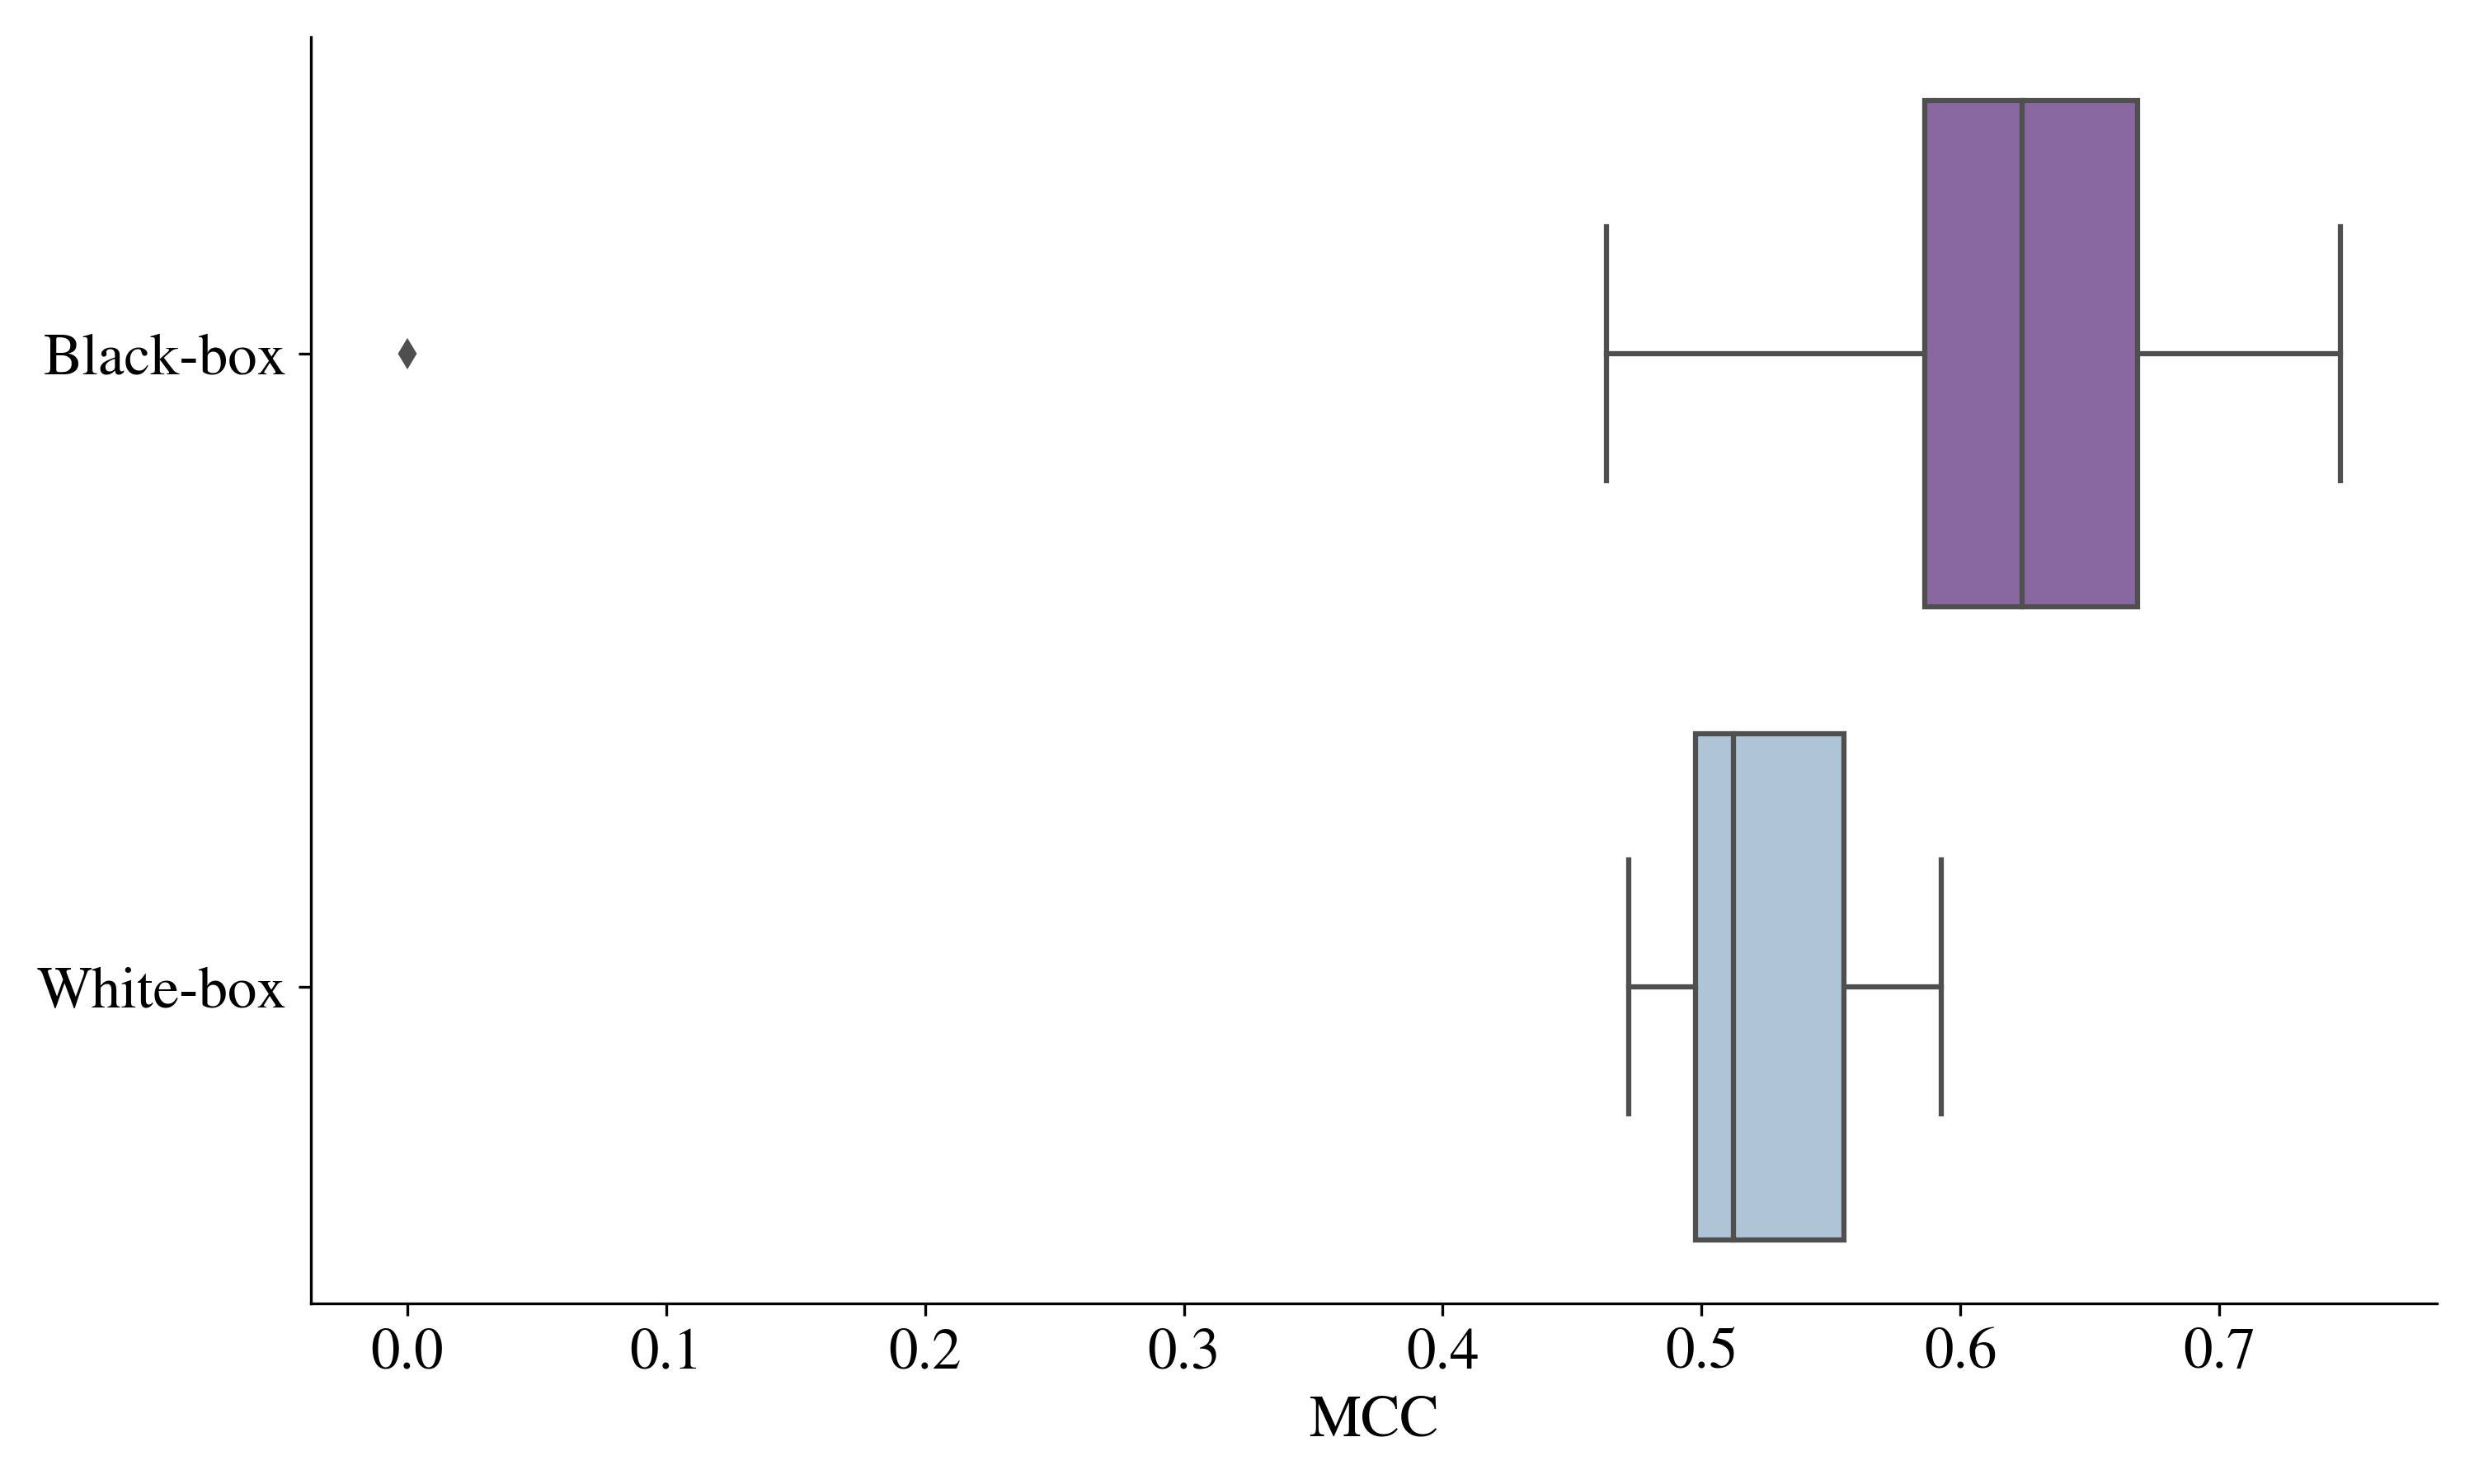
\includegraphics[width=140mm]{Figures/MCC_Distribution_BB_WB.jpg}
    
    \centering{\begin{source}Author's results in Python\end{source}}\vspace{-1em}
\end{figure}

\begin{figure}[H]
    \centering
    \caption{Matthews Correlation Coefficient Distribution (Black--box/White--box dimension) - \textit{without outlier}}\vspace{0.5em}
    \label{fig:mccdistwooutbbwb}
    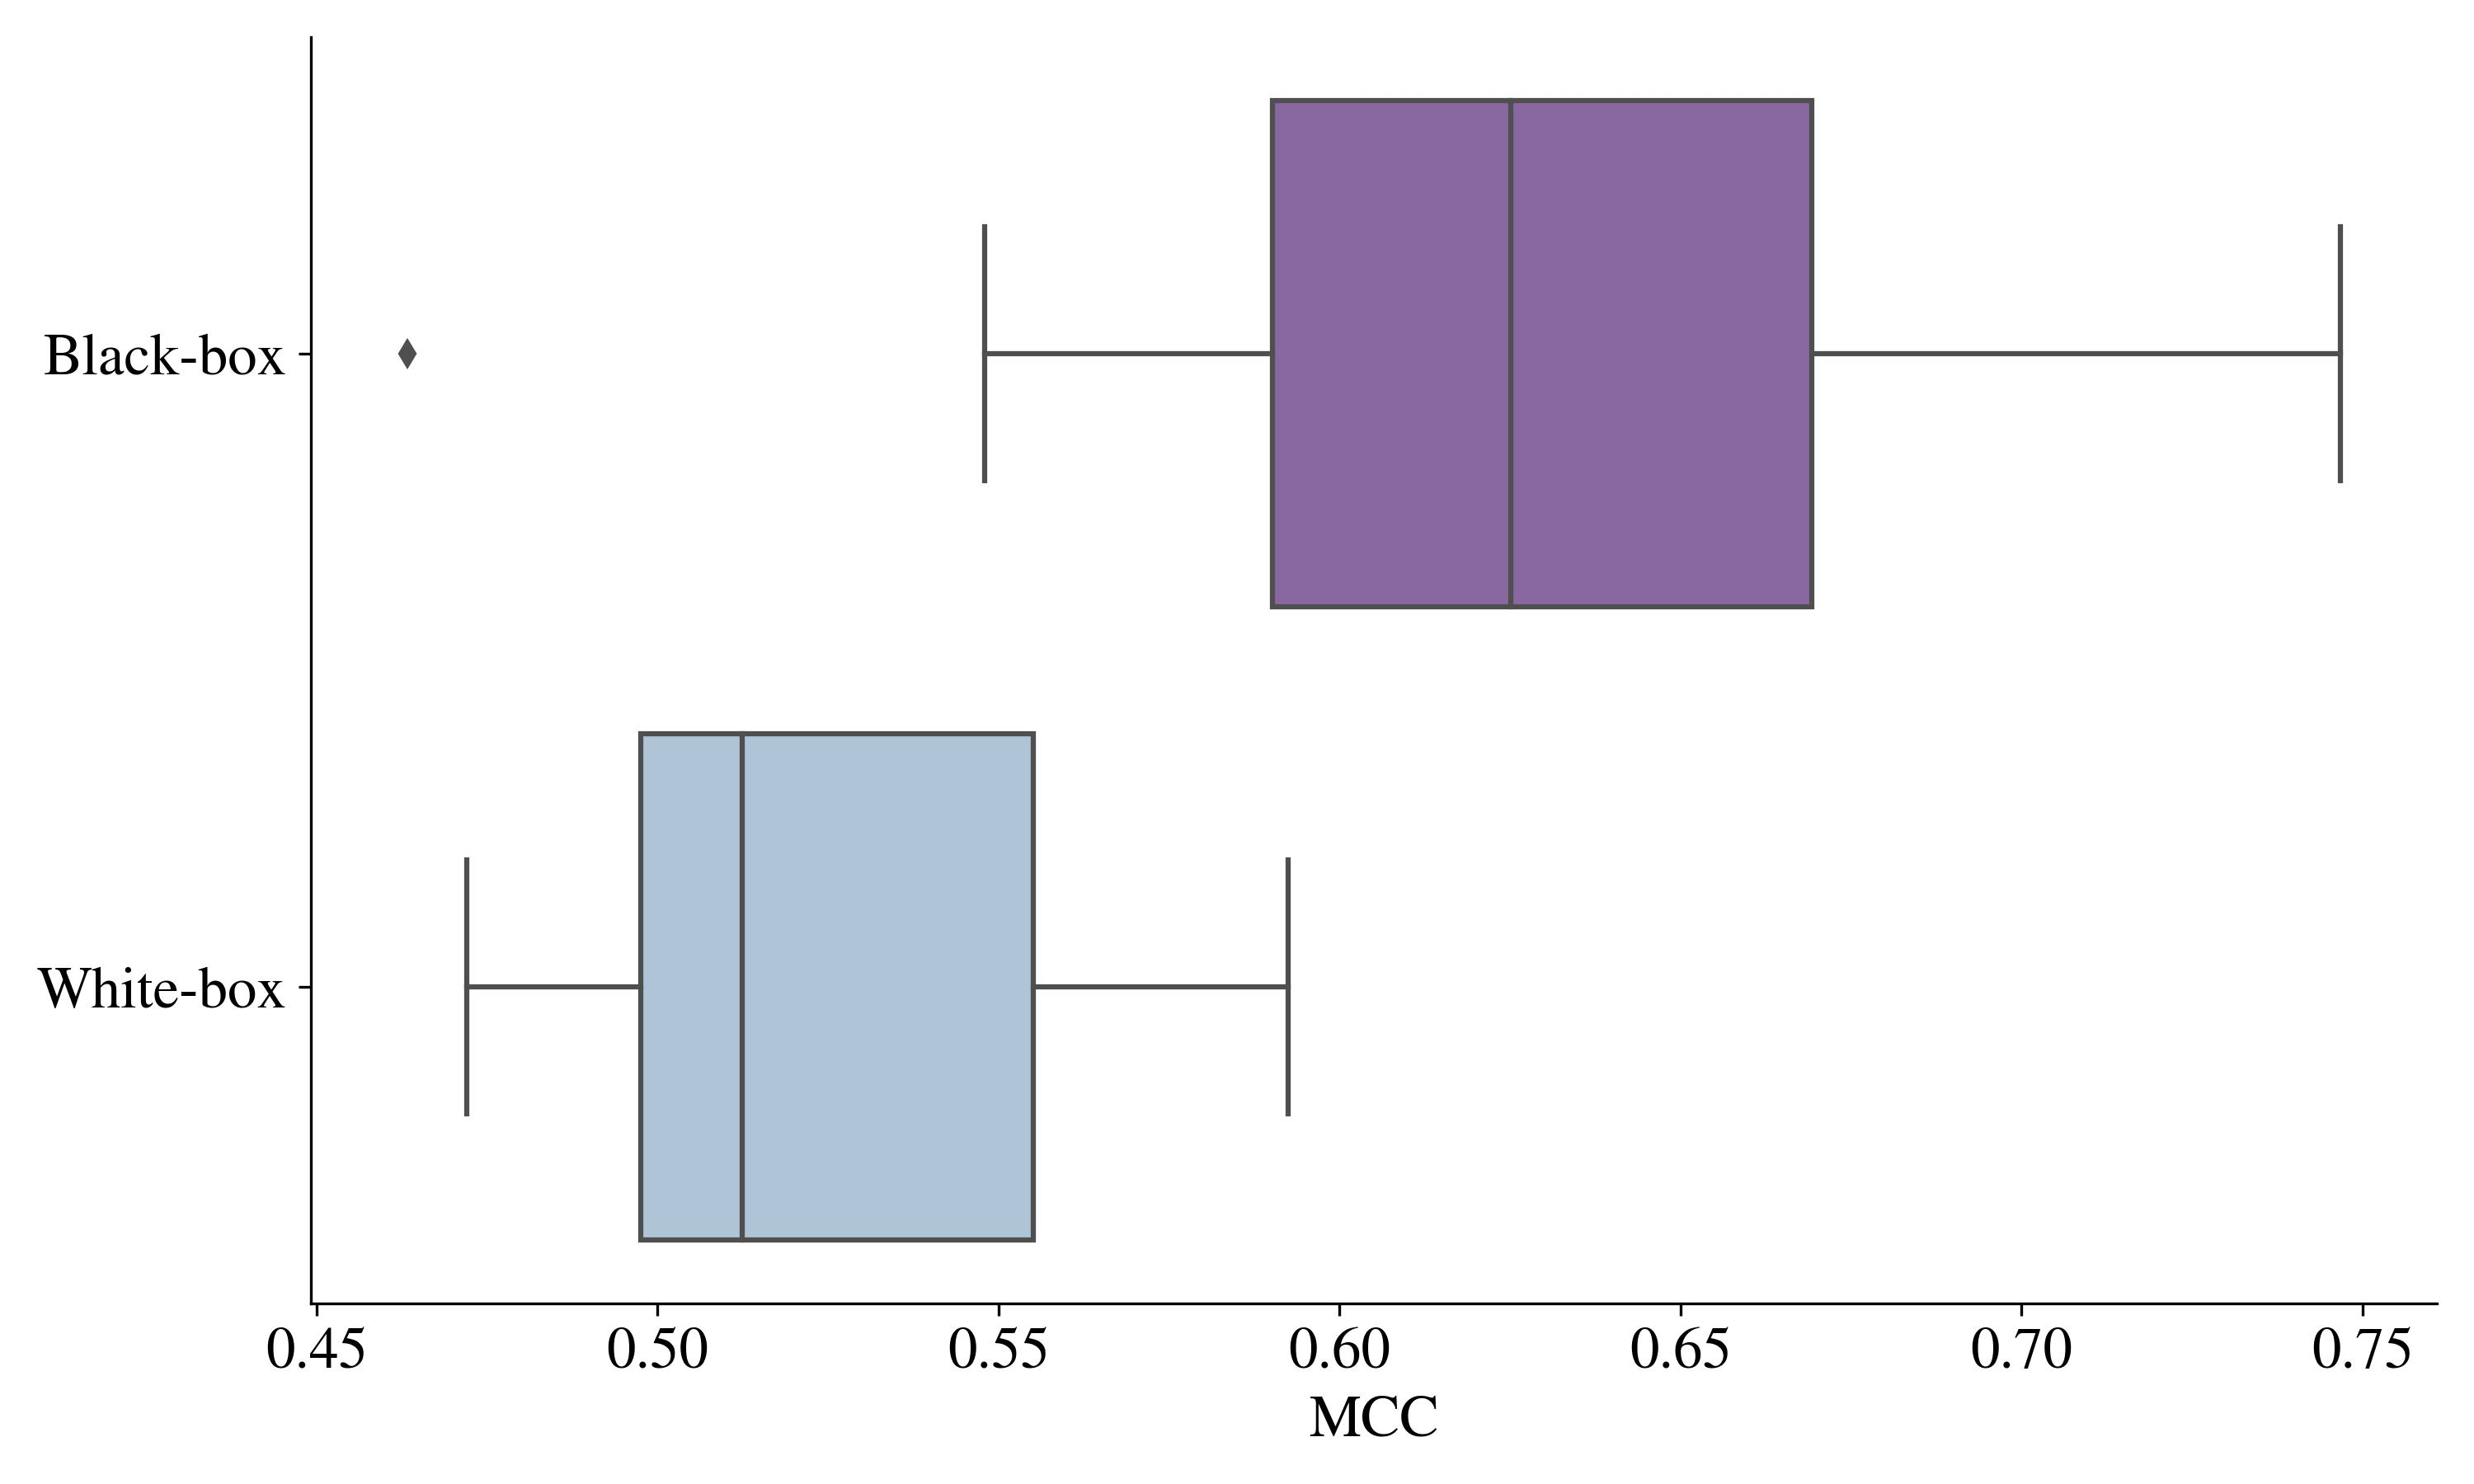
\includegraphics[width=140mm]{Figures/MCC_WO_OUTLIERS_Distribution_BB_WB.jpg}
    
    \centering{\begin{source}Author's results in Python\end{source}}\vspace{-1em}
\end{figure}

\begin{figure}[H]
    \centering
    \caption{Brier Score Loss Distribution}\vspace{0.5em}
    \label{fig:bsldist}
    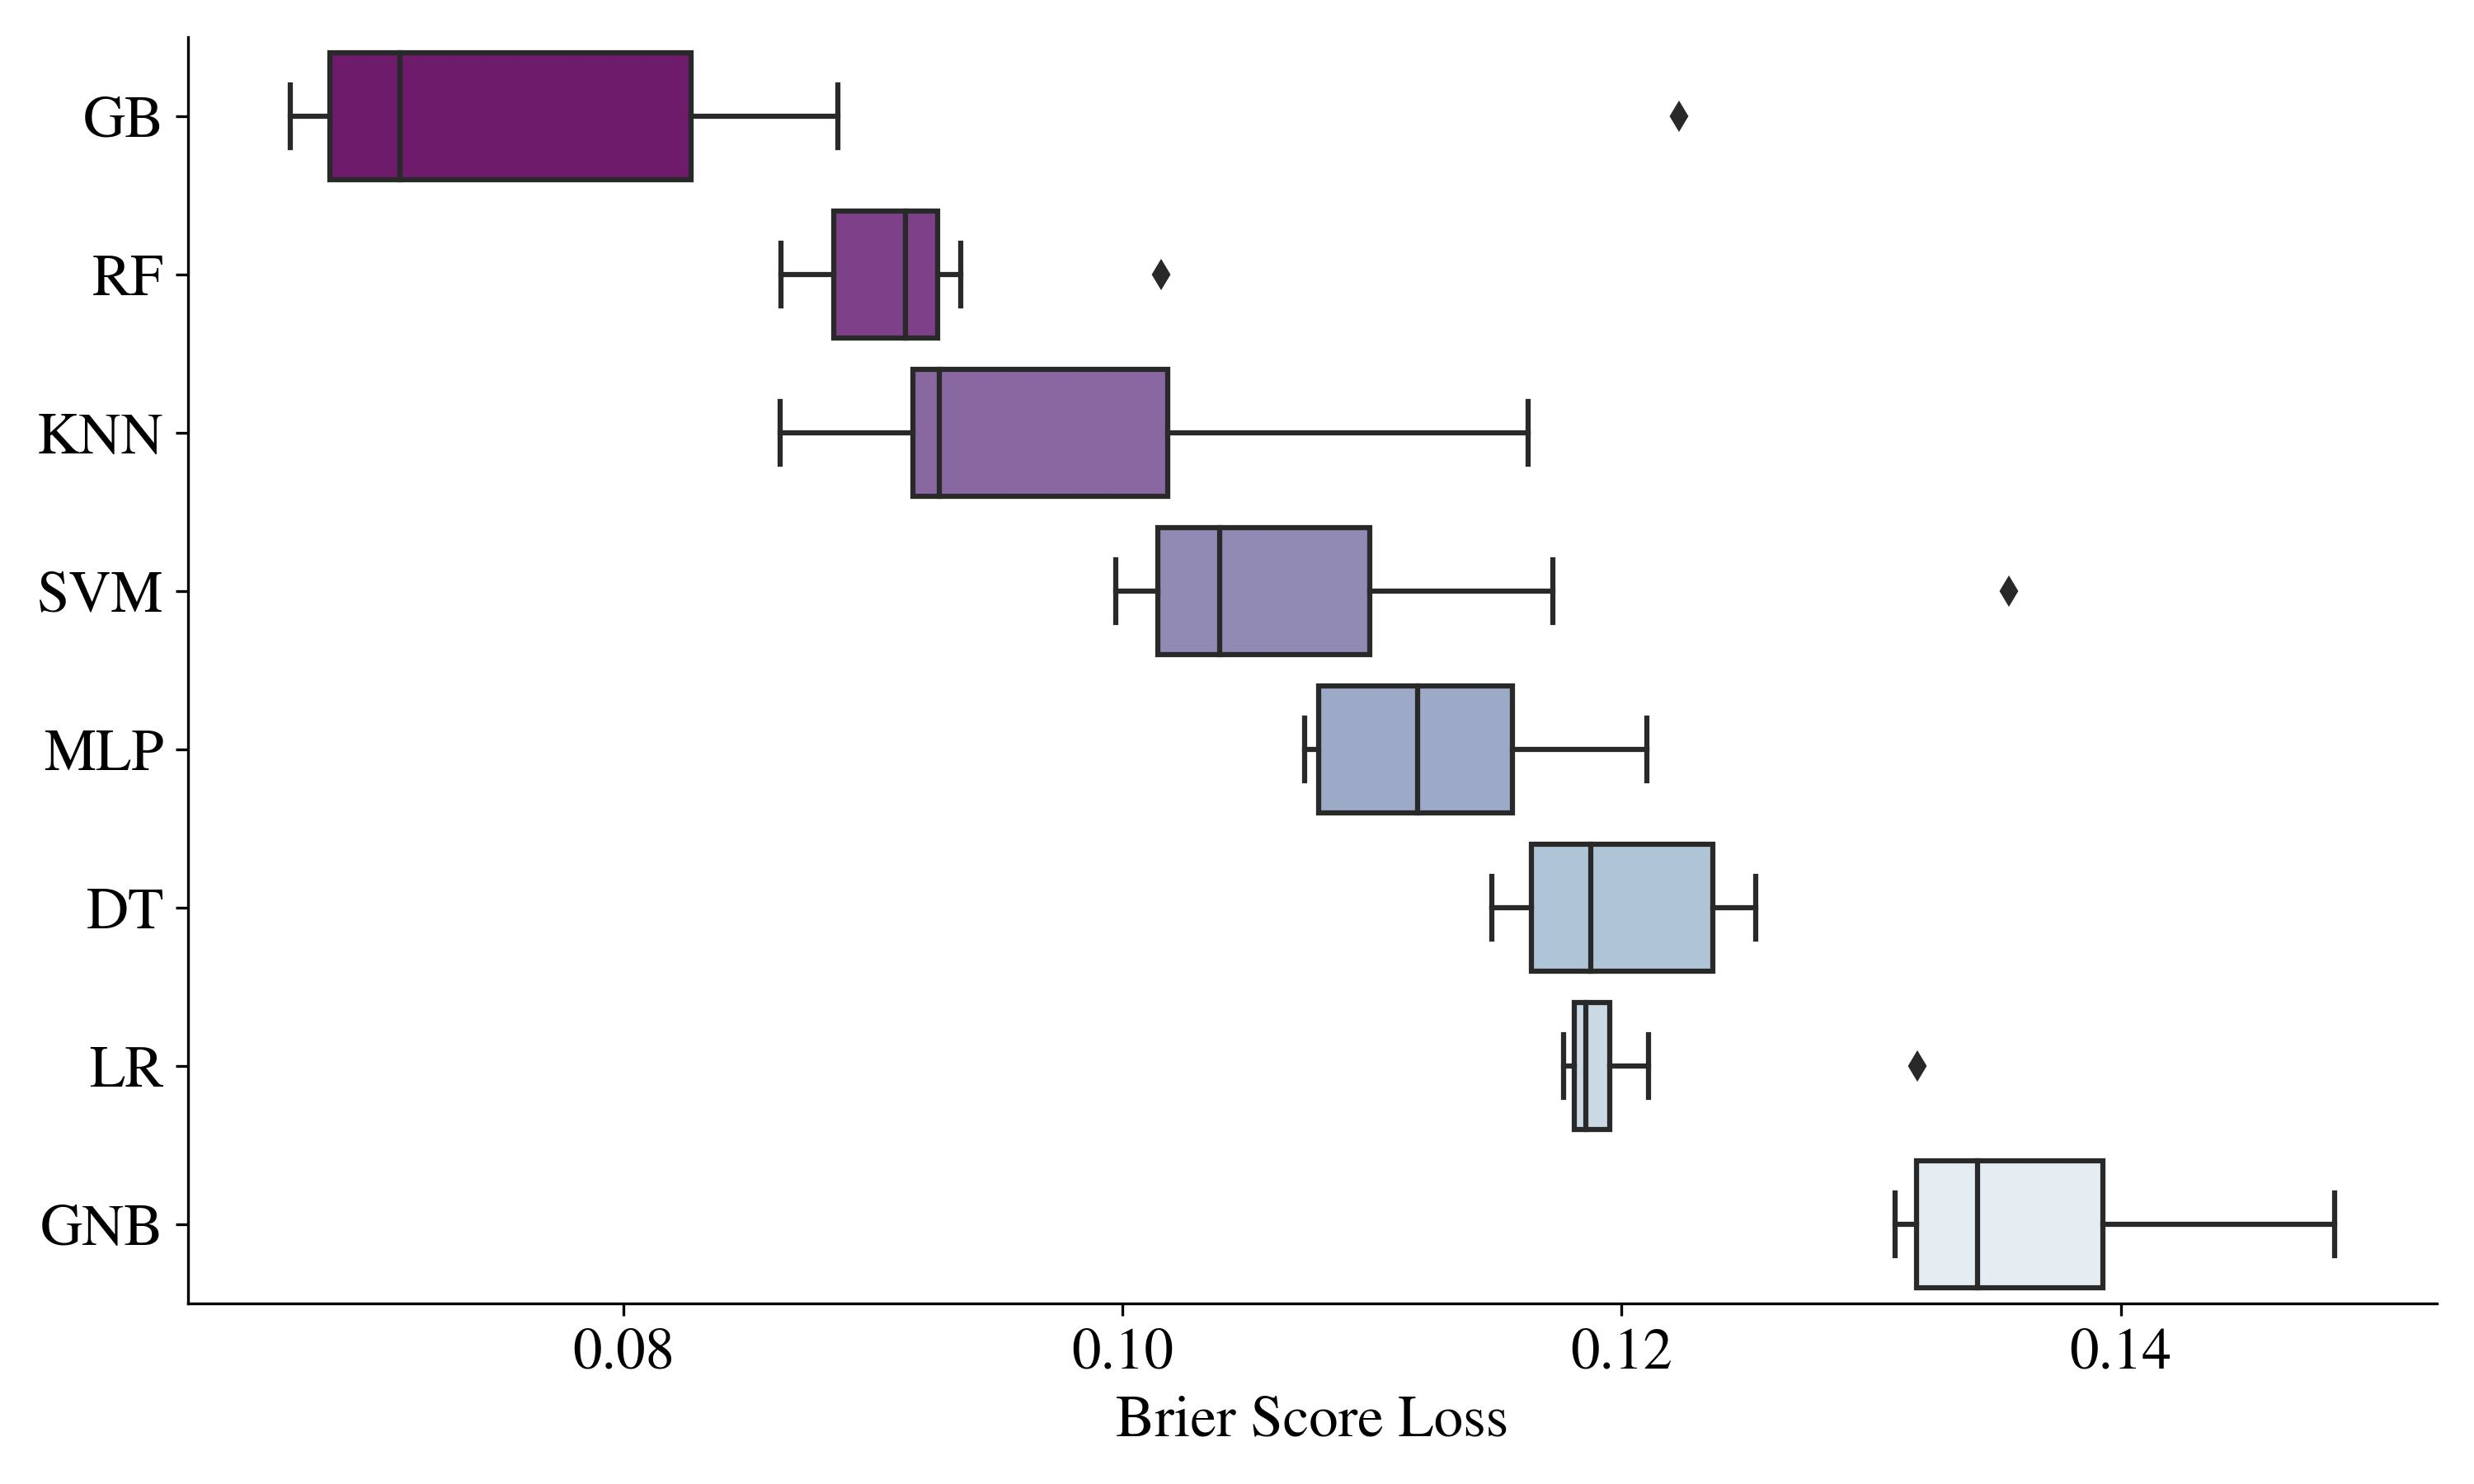
\includegraphics[width=140mm]{Figures/BRIER SCORE LOSS_Distribution.jpg}
    
    \centering{\begin{source}Author's results in Python\end{source}}\vspace{-1em}
\end{figure}

\begin{figure}[H]
    \centering
    \caption{Brier Score Loss Distribution (Black--box/White--box dimension)}\vspace{0.5em}
    \label{fig:bsldistbbwb}
    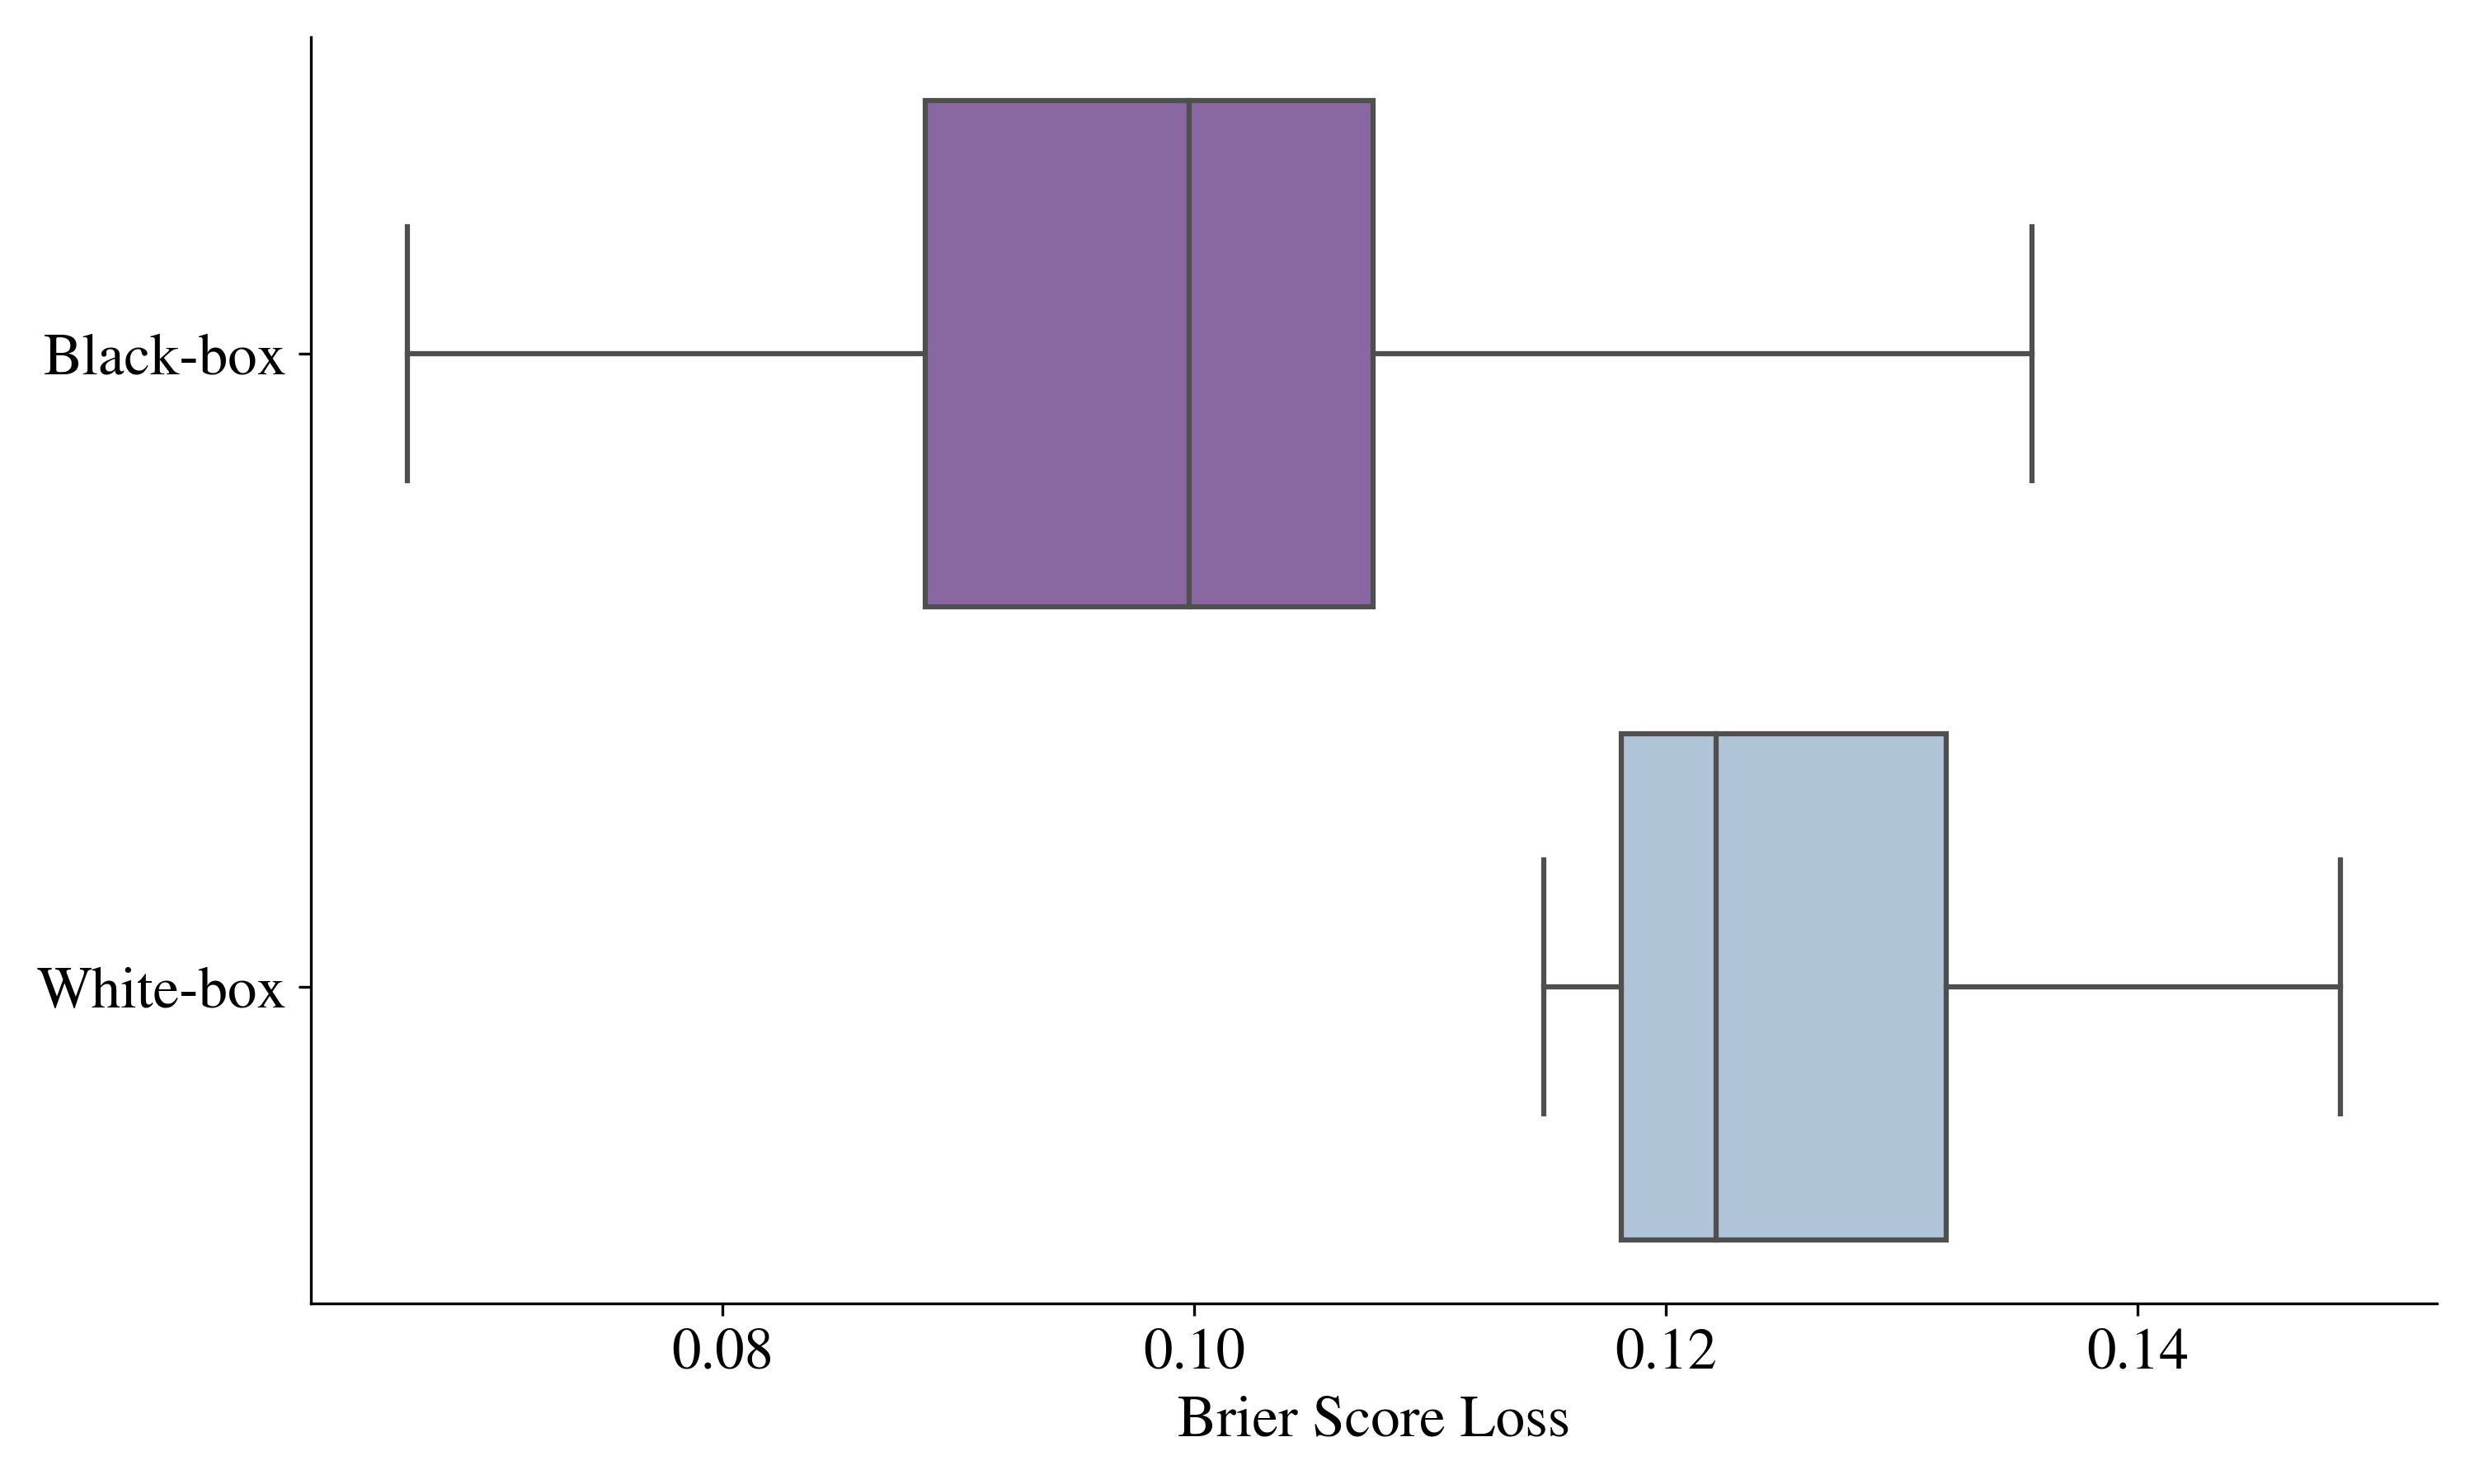
\includegraphics[width=140mm]{Figures/BRIER SCORE LOSS_Distribution_BB_WB.jpg}
    
    \centering{\begin{source}Author's results in Python\end{source}}\vspace{-1em}
\end{figure}

\begin{figure}[H]
    \centering
    \caption{Kolmogorov--Smirnov Distance Distribution}\vspace{0.5em}
    \label{fig:ksdist}
    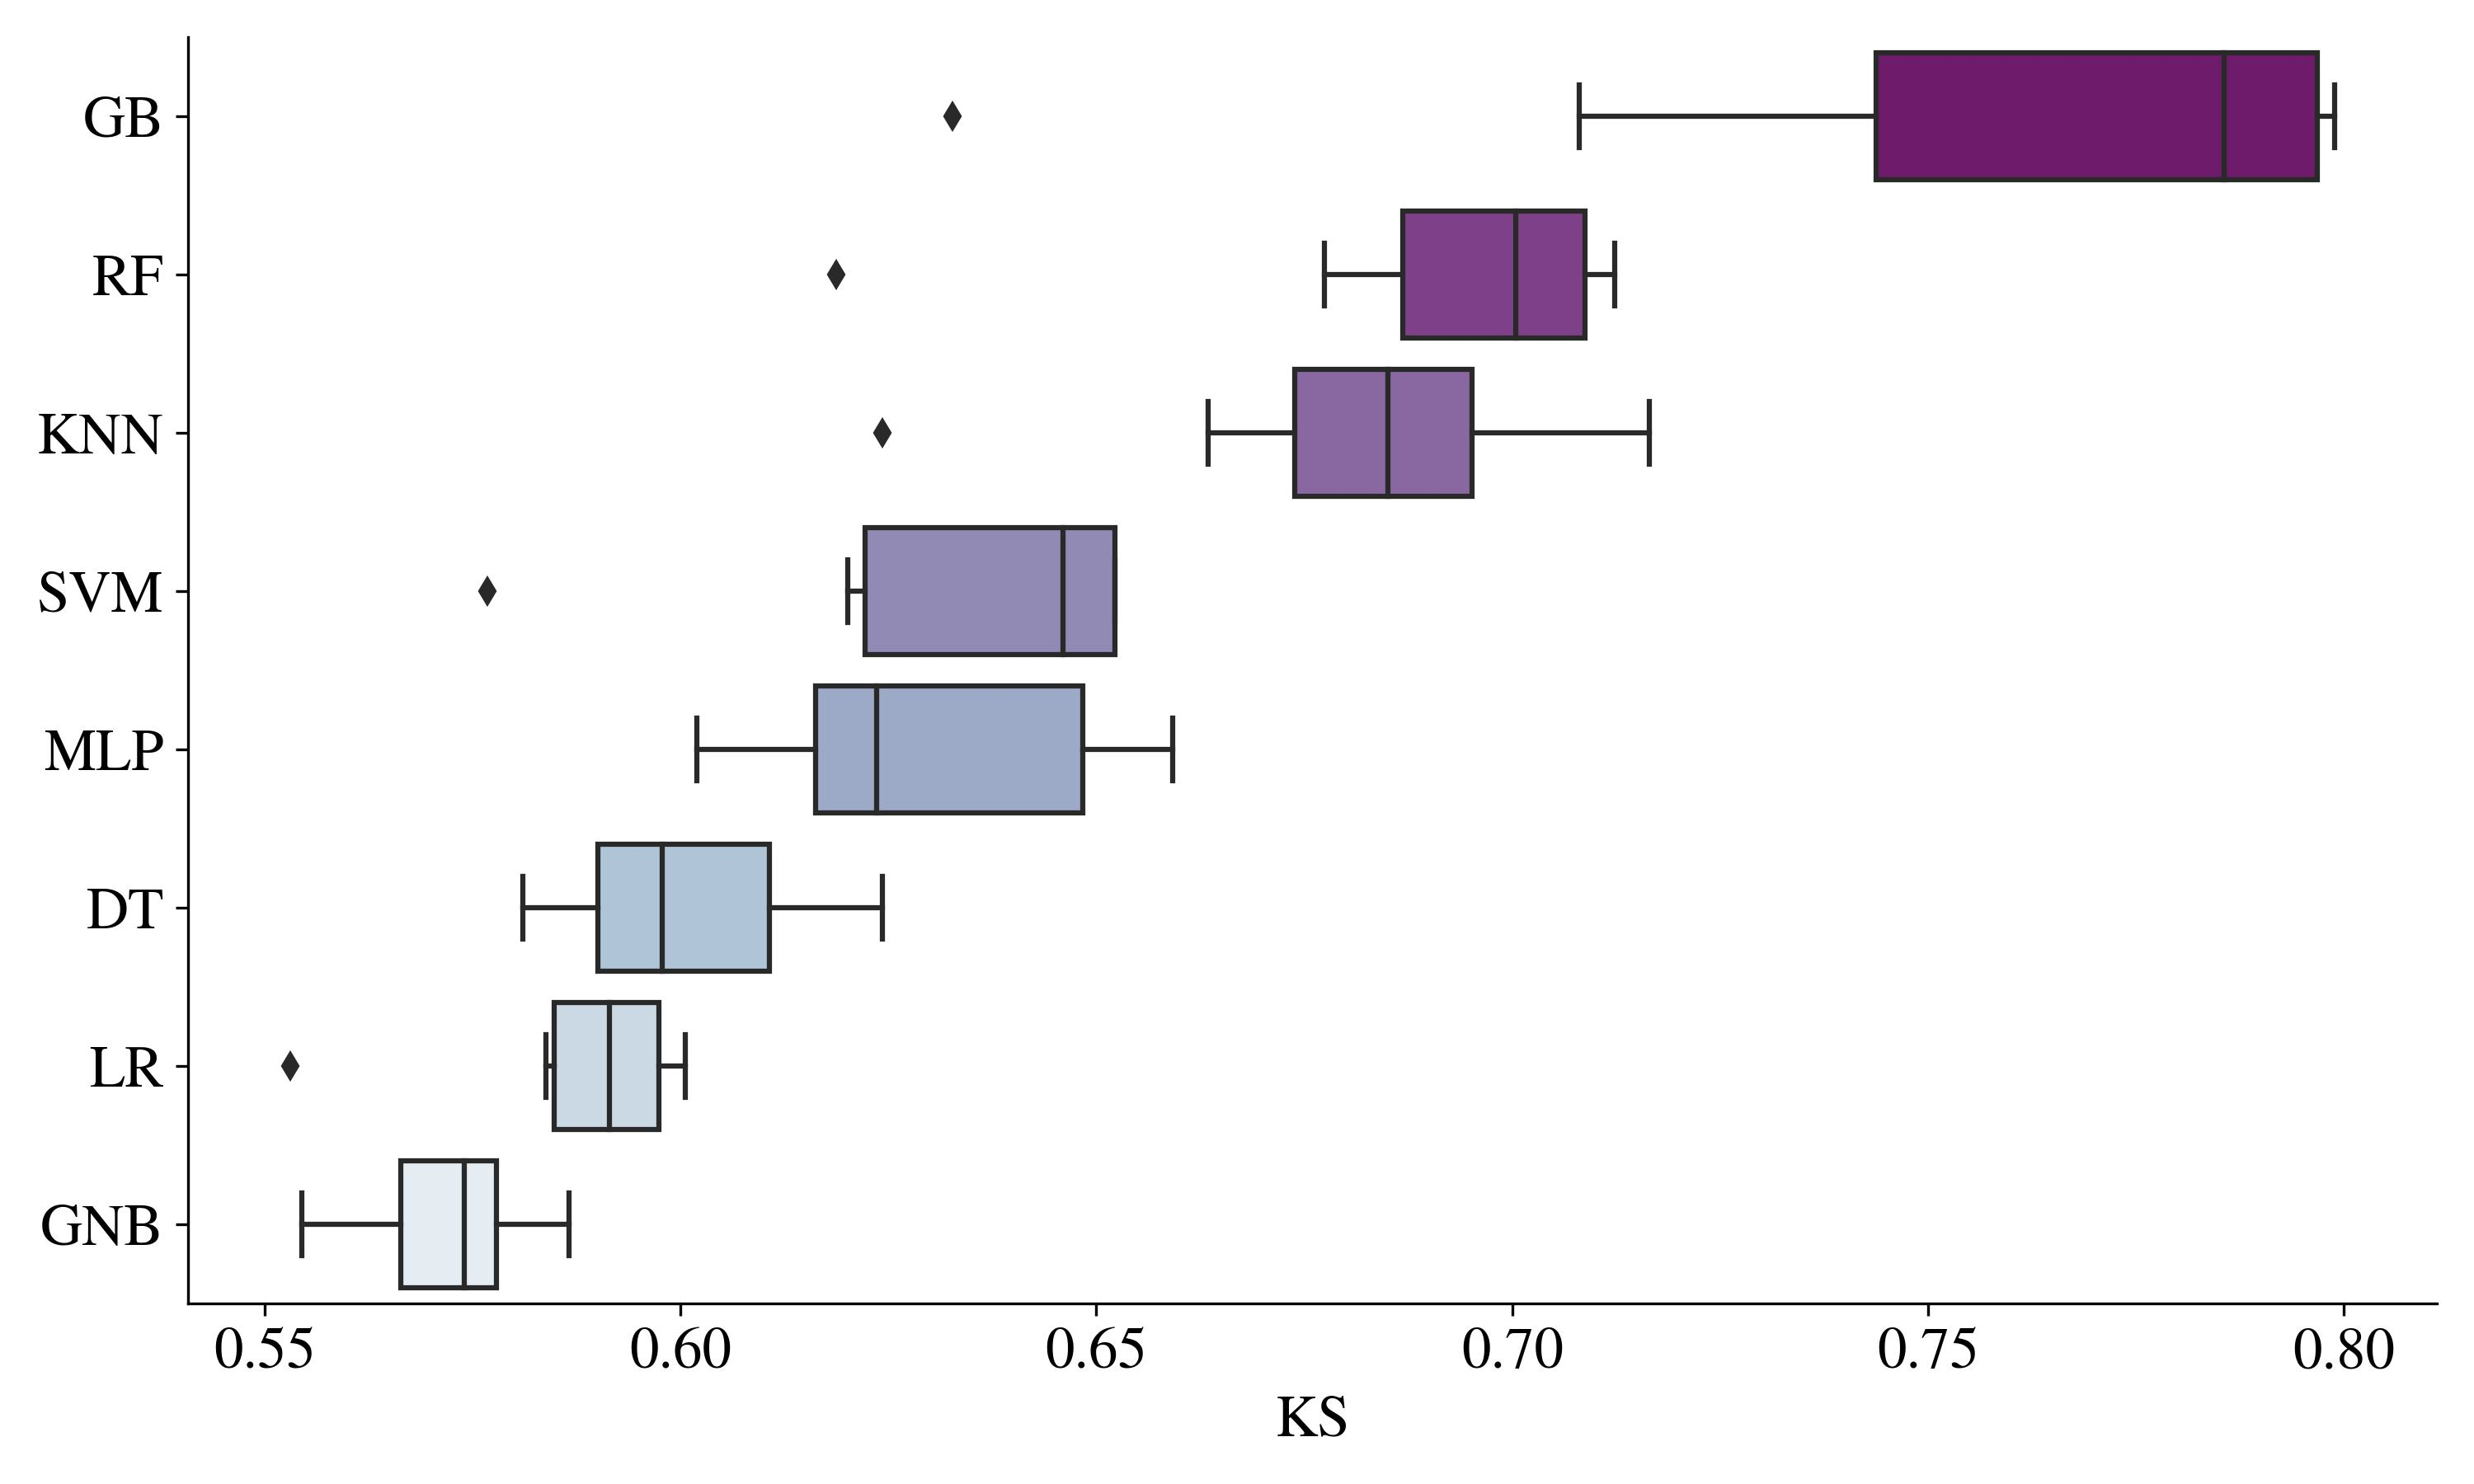
\includegraphics[width=140mm]{Figures/KS_Distribution.jpg}
    
    \centering{\begin{source}Author's results in Python\end{source}}\vspace{-1em}
\end{figure}

\begin{figure}[H]
    \centering
    \caption{Kolmogorov--Smirnov Distance Distribution (Black--box/White--box dimension)}\vspace{0.5em}
    \label{fig:ksdistbbwb}
    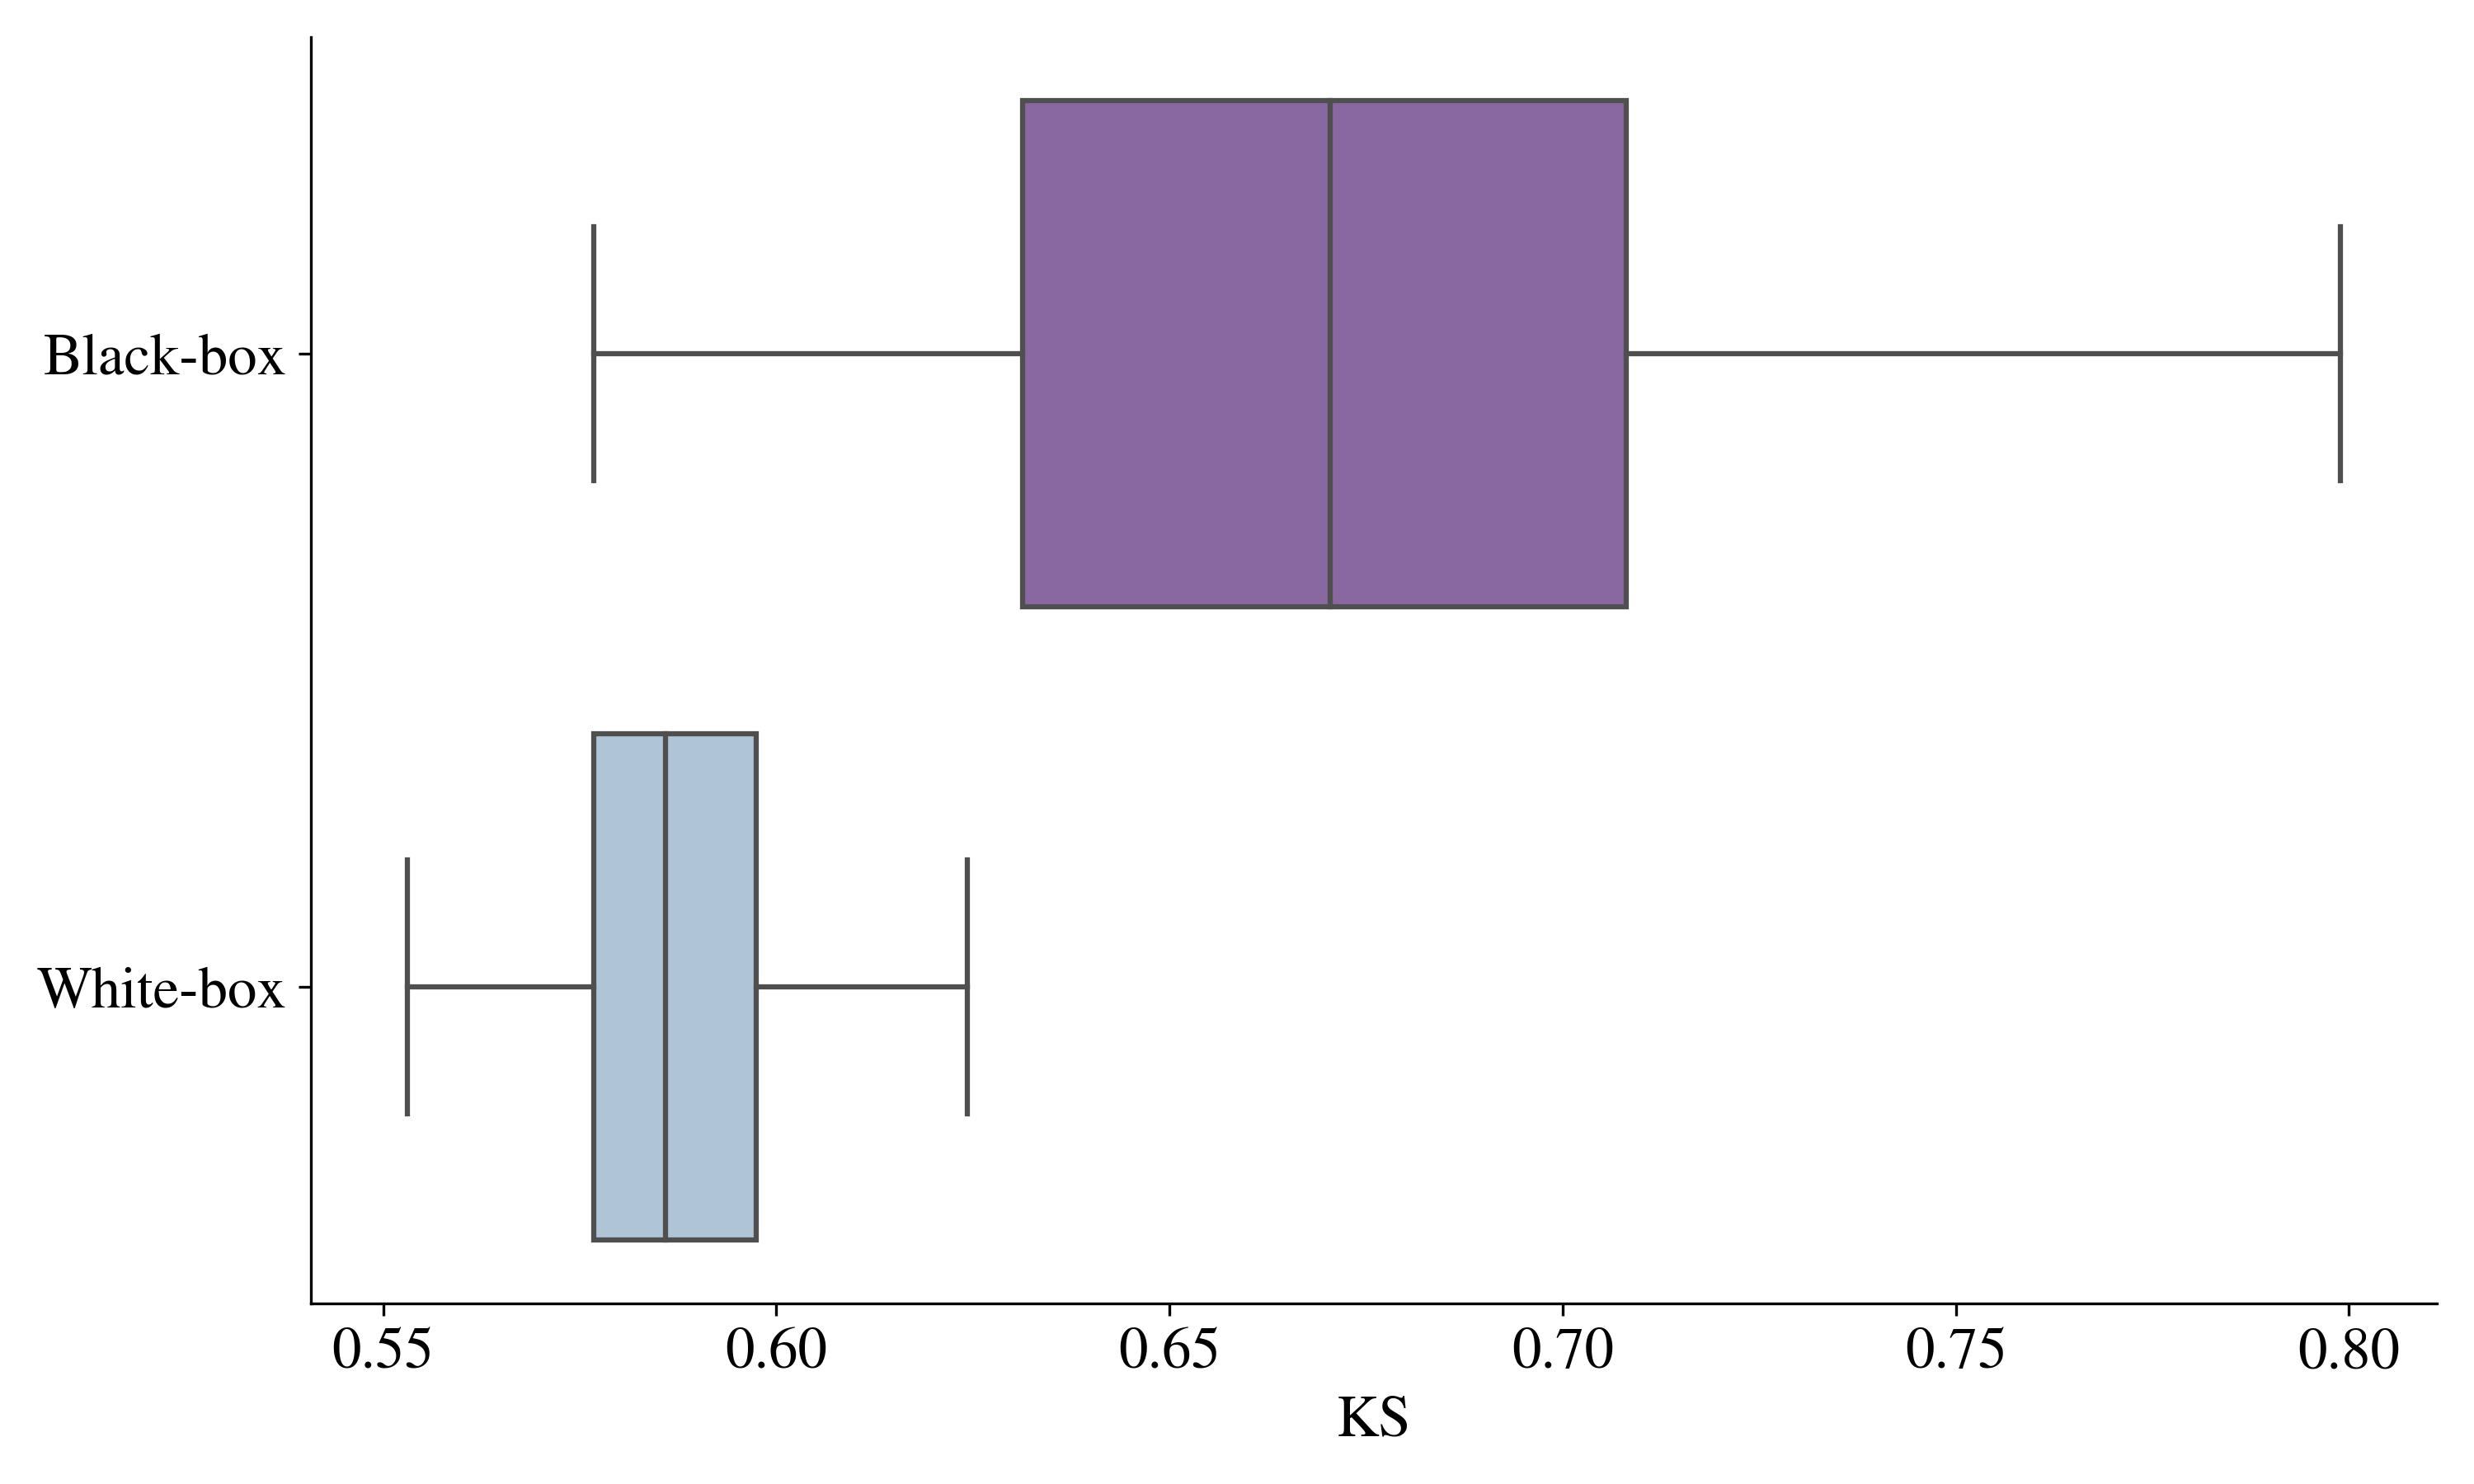
\includegraphics[width=140mm]{Figures/KS_Distribution_BB_WB.jpg}
    
    \centering{\begin{source}Author's results in Python\end{source}}\vspace{-1em}
\end{figure}

\begin{figure}[H]
    \centering
    \caption{Log Loss Distribution}\vspace{0.5em}
    \label{fig:loglossdist}
    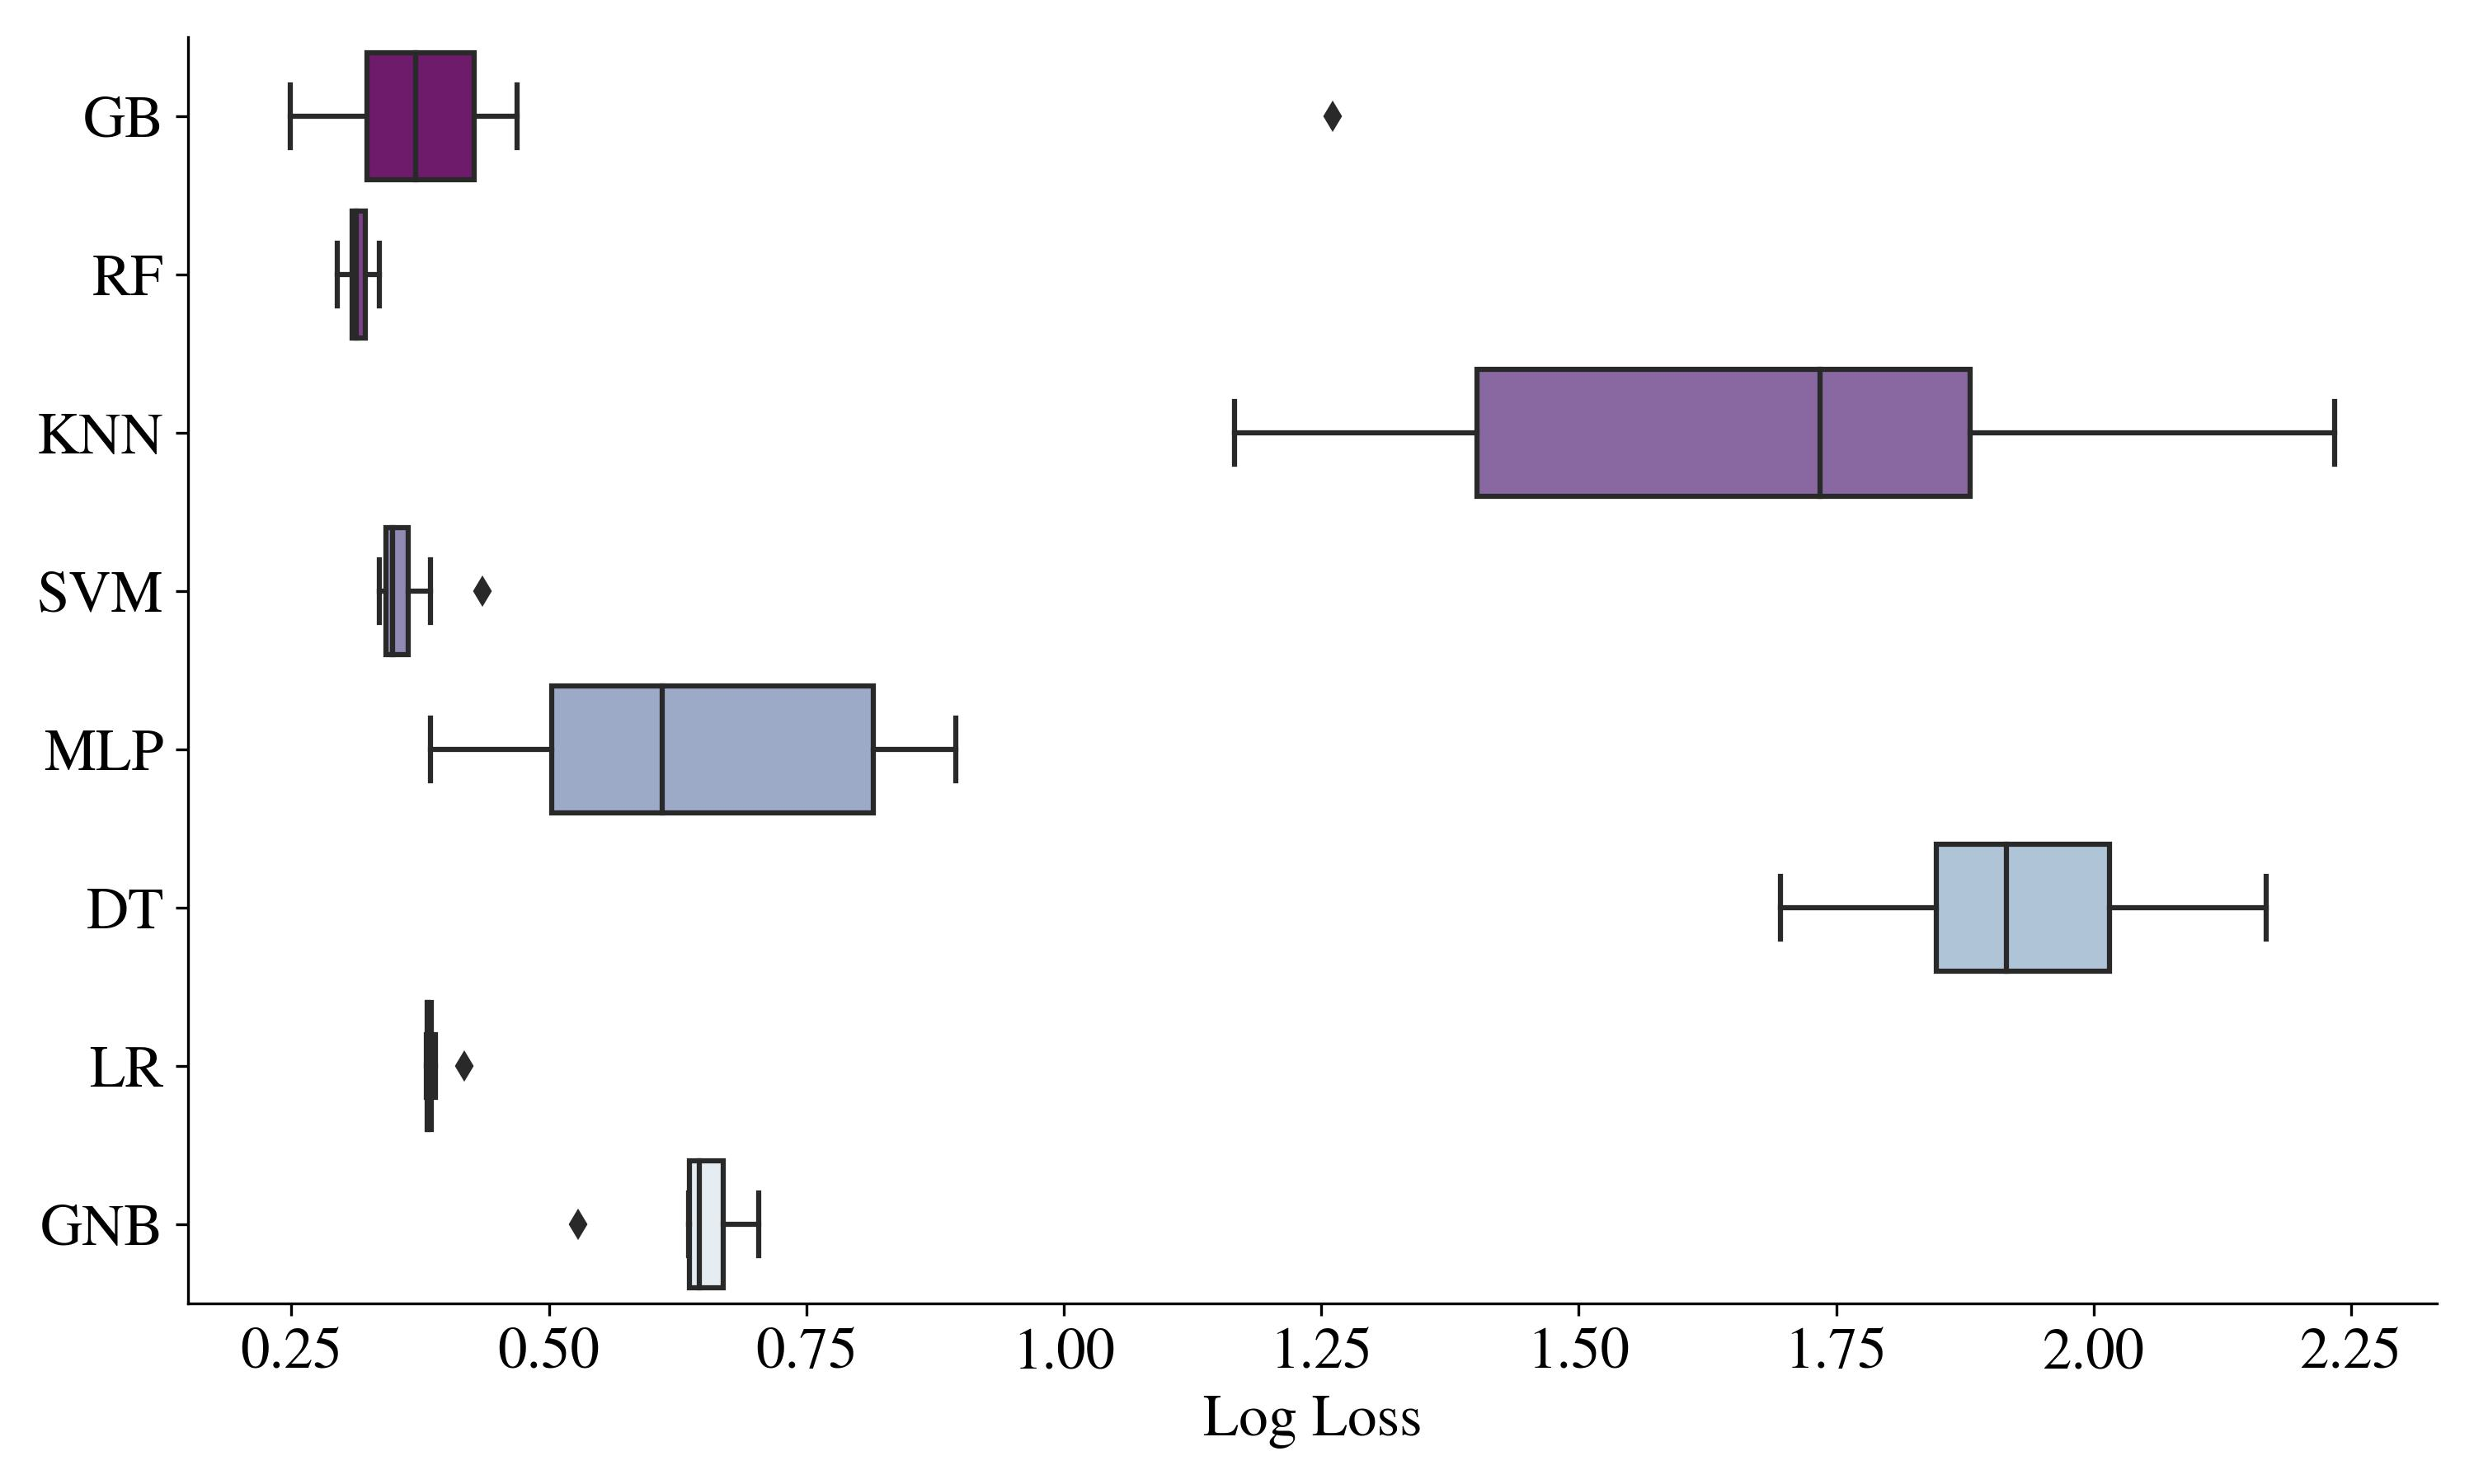
\includegraphics[width=140mm]{Figures/LOG LOSS_Distribution.jpg}
    
    \centering{\begin{source}Author's results in Python\end{source}}\vspace{-1em}
\end{figure}

\begin{figure}[H]
    \centering
    \caption{Log Loss Distribution (Black--box/White--box dimension)}\vspace{0.5em}
    \label{fig:loglossdistbbwb}
    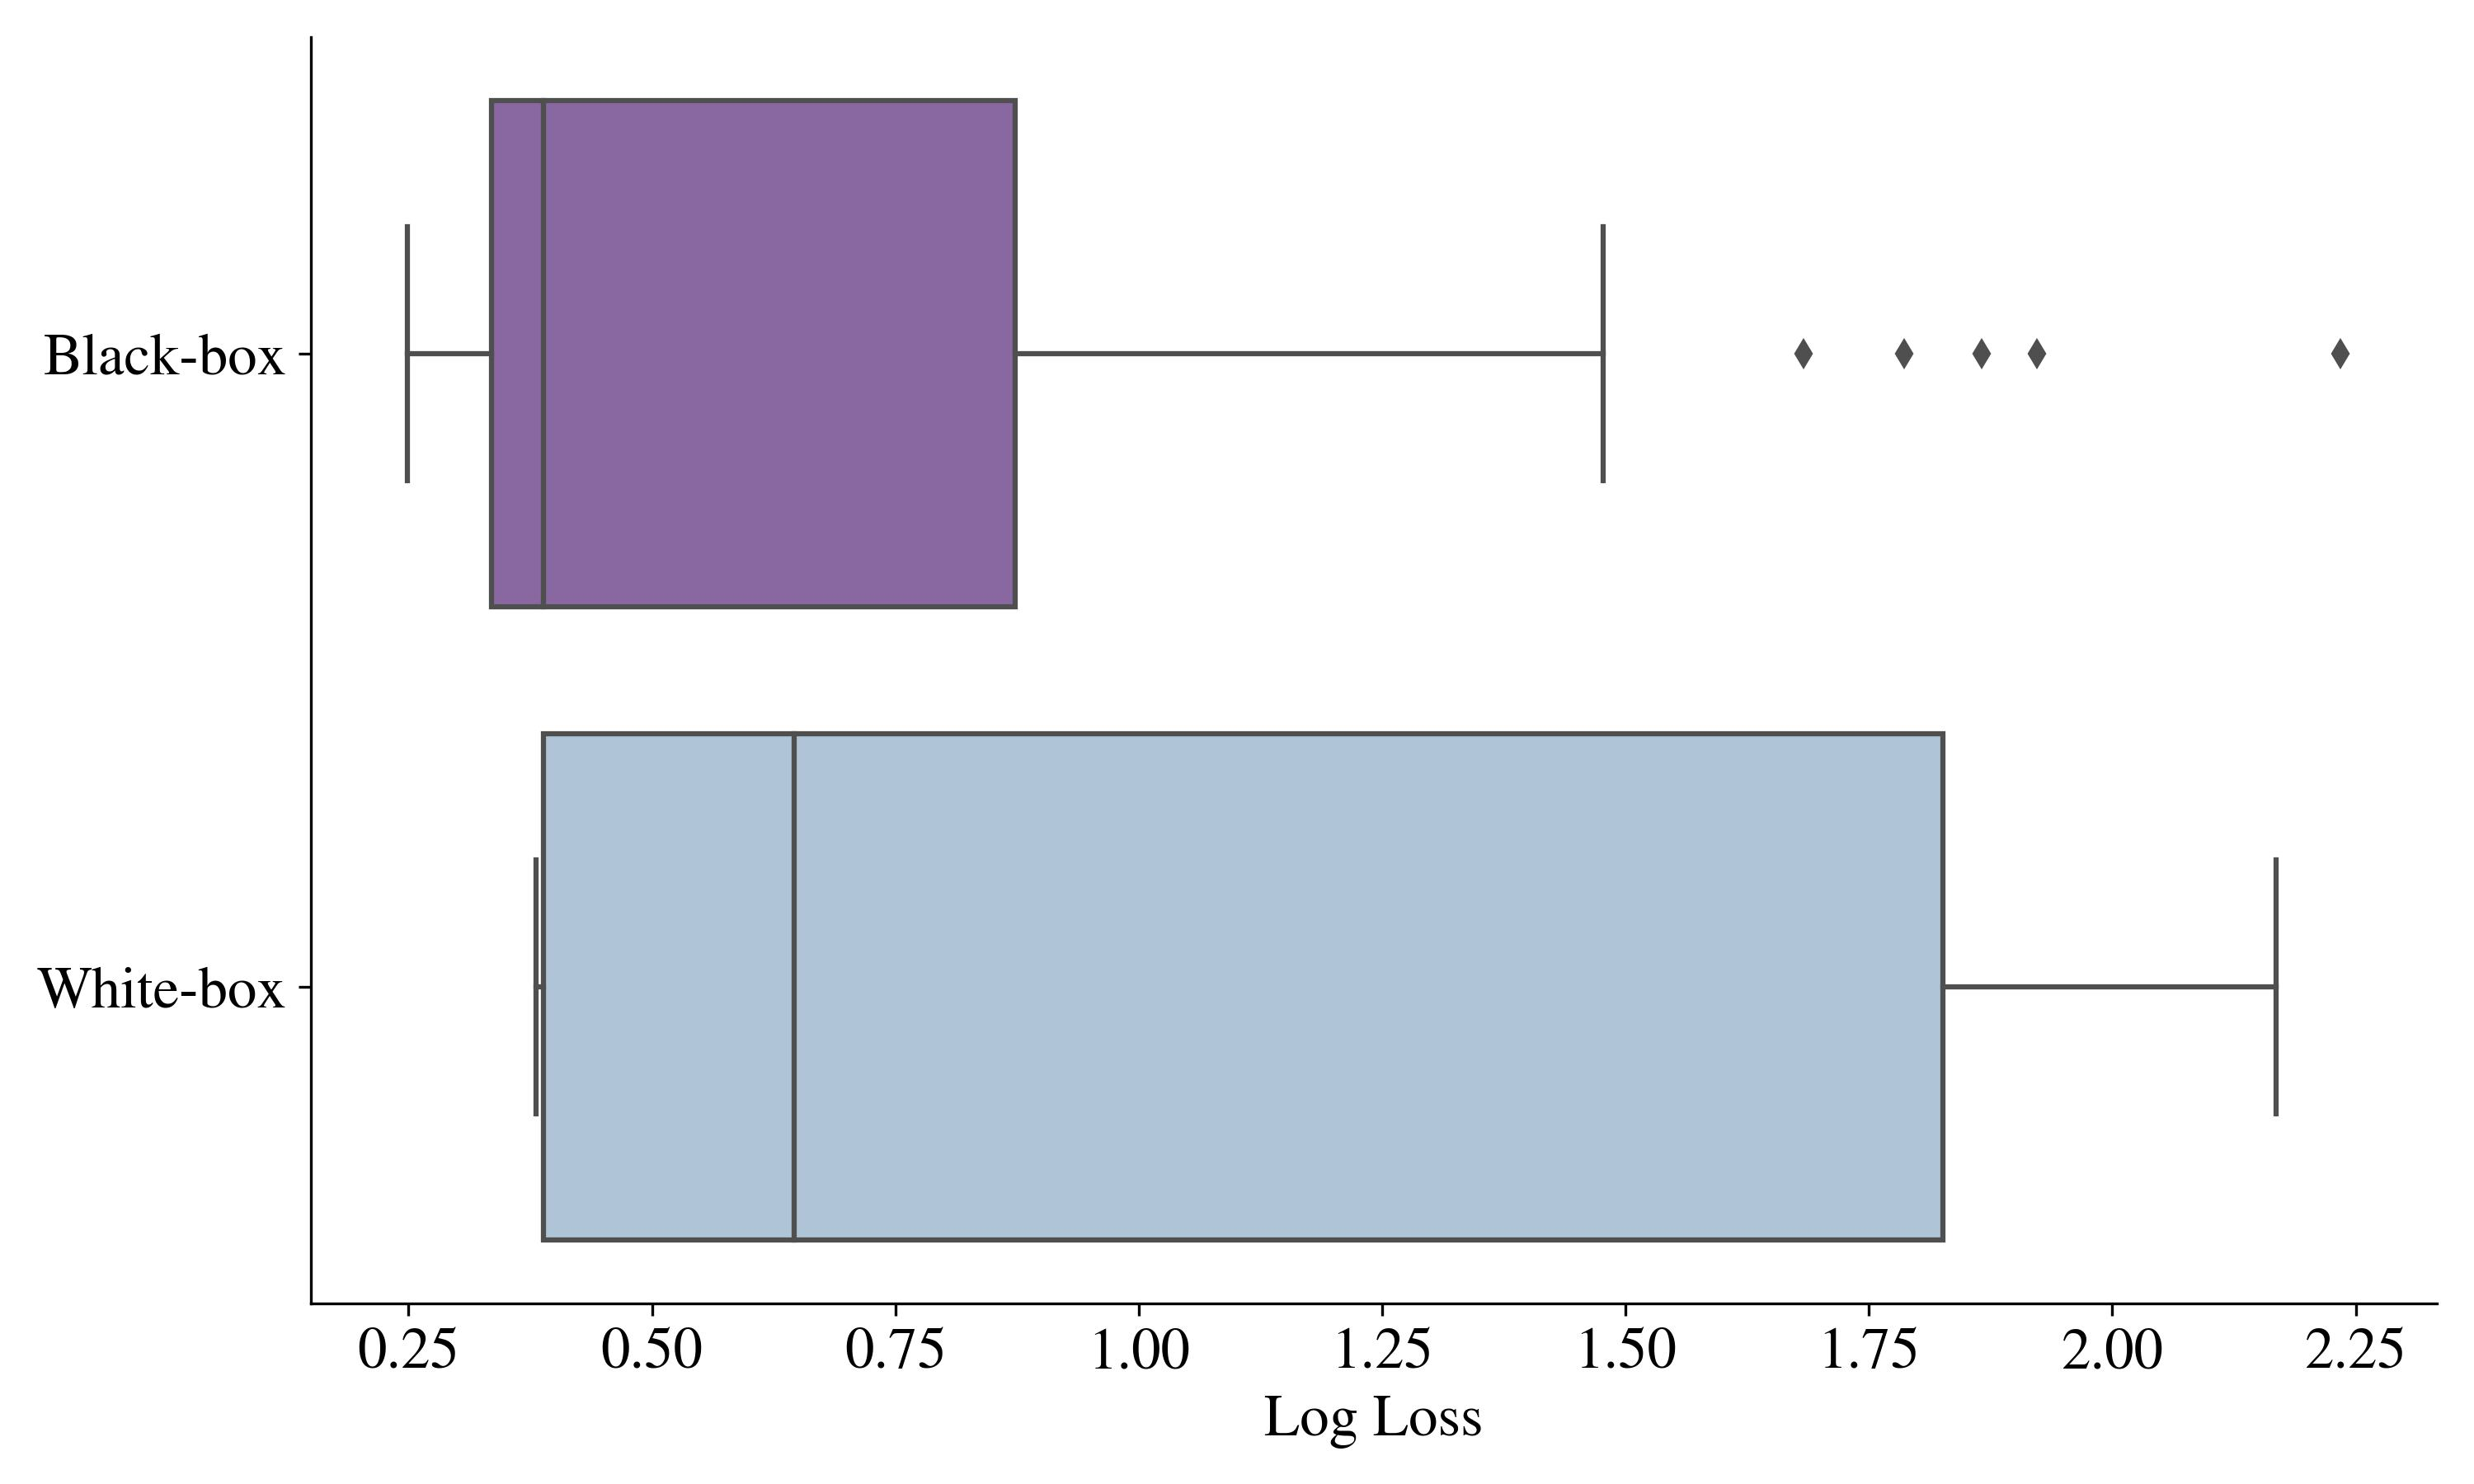
\includegraphics[width=140mm]{Figures/LOG LOSS_Distribution_BB_WB.jpg}
    
    \centering{\begin{source}Author's results in Python\end{source}}\vspace{-1em}
\end{figure}

\begin{figure}[H]
    \centering
    \caption{Somers' D Distribution}\vspace{0.5em}
    \label{fig:sddist}
    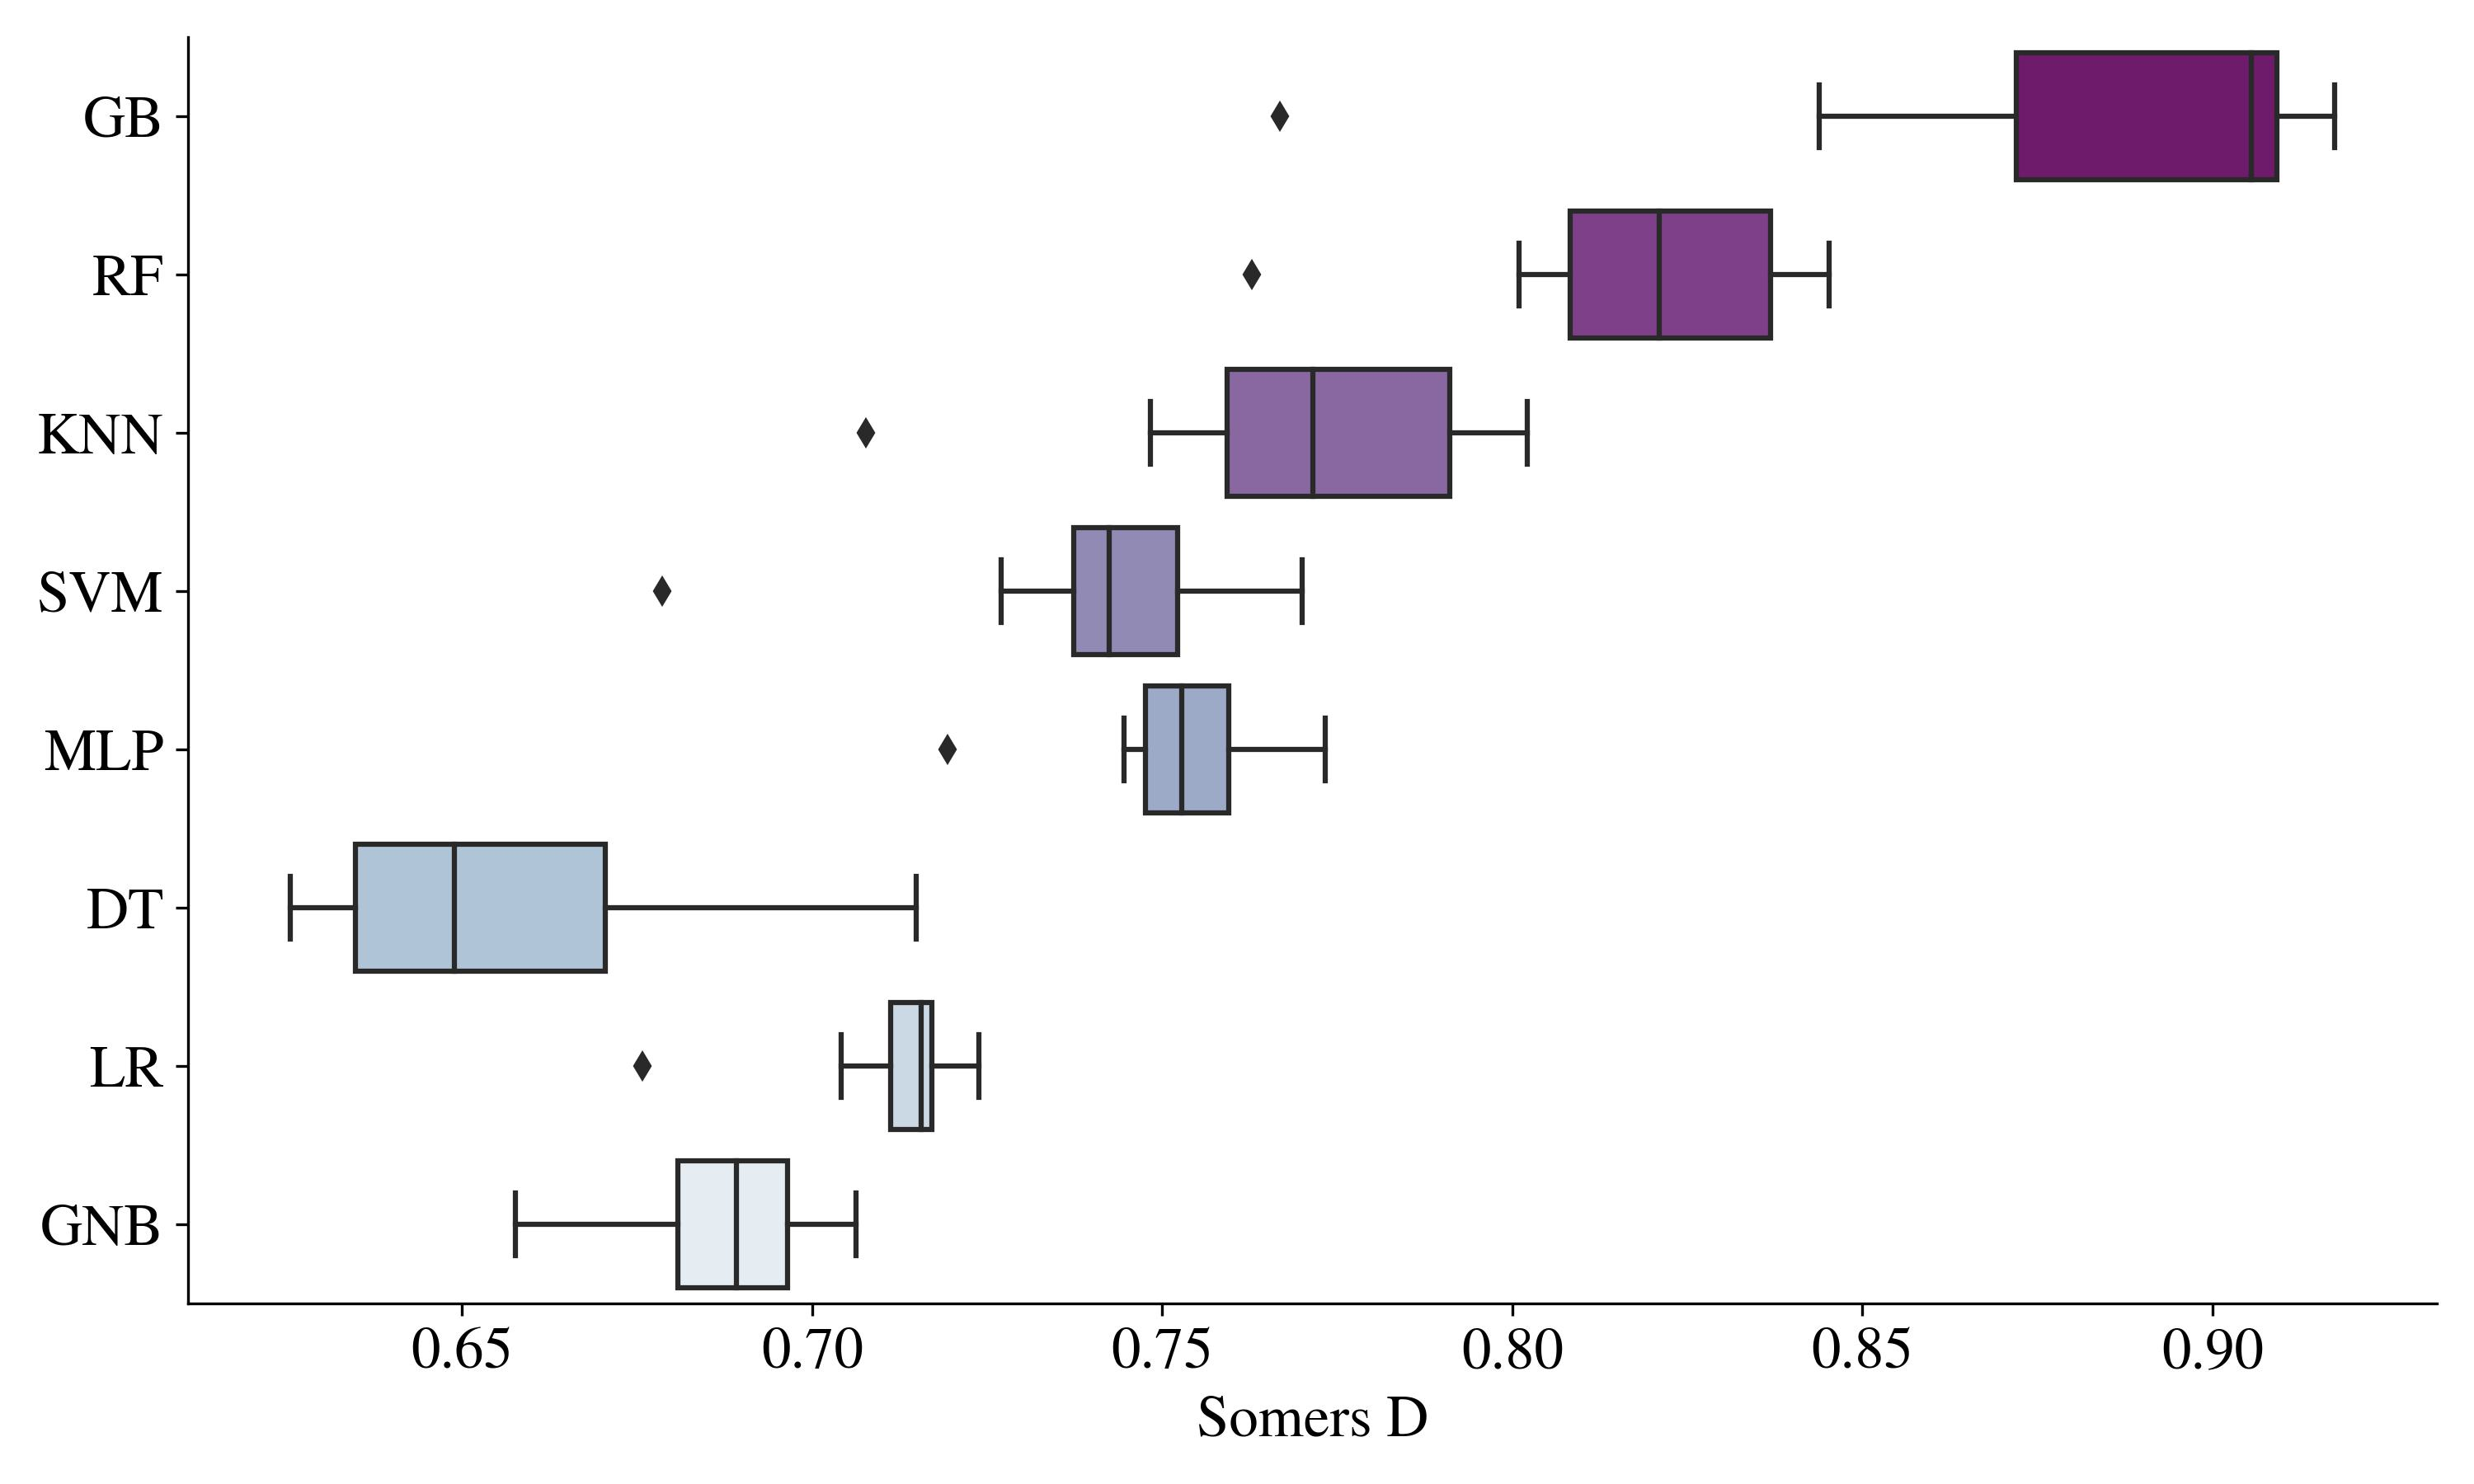
\includegraphics[width=140mm]{Figures/SOMERS D_Distribution.jpg}
    
    \centering{\begin{source}Author's results in Python\end{source}}\vspace{-1em}
\end{figure}

\begin{figure}[H]
    \centering
    \caption{Somers' D Distribution (Black--box/White--box dimension)}\vspace{0.5em}
    \label{fig:sddistbbwb}
    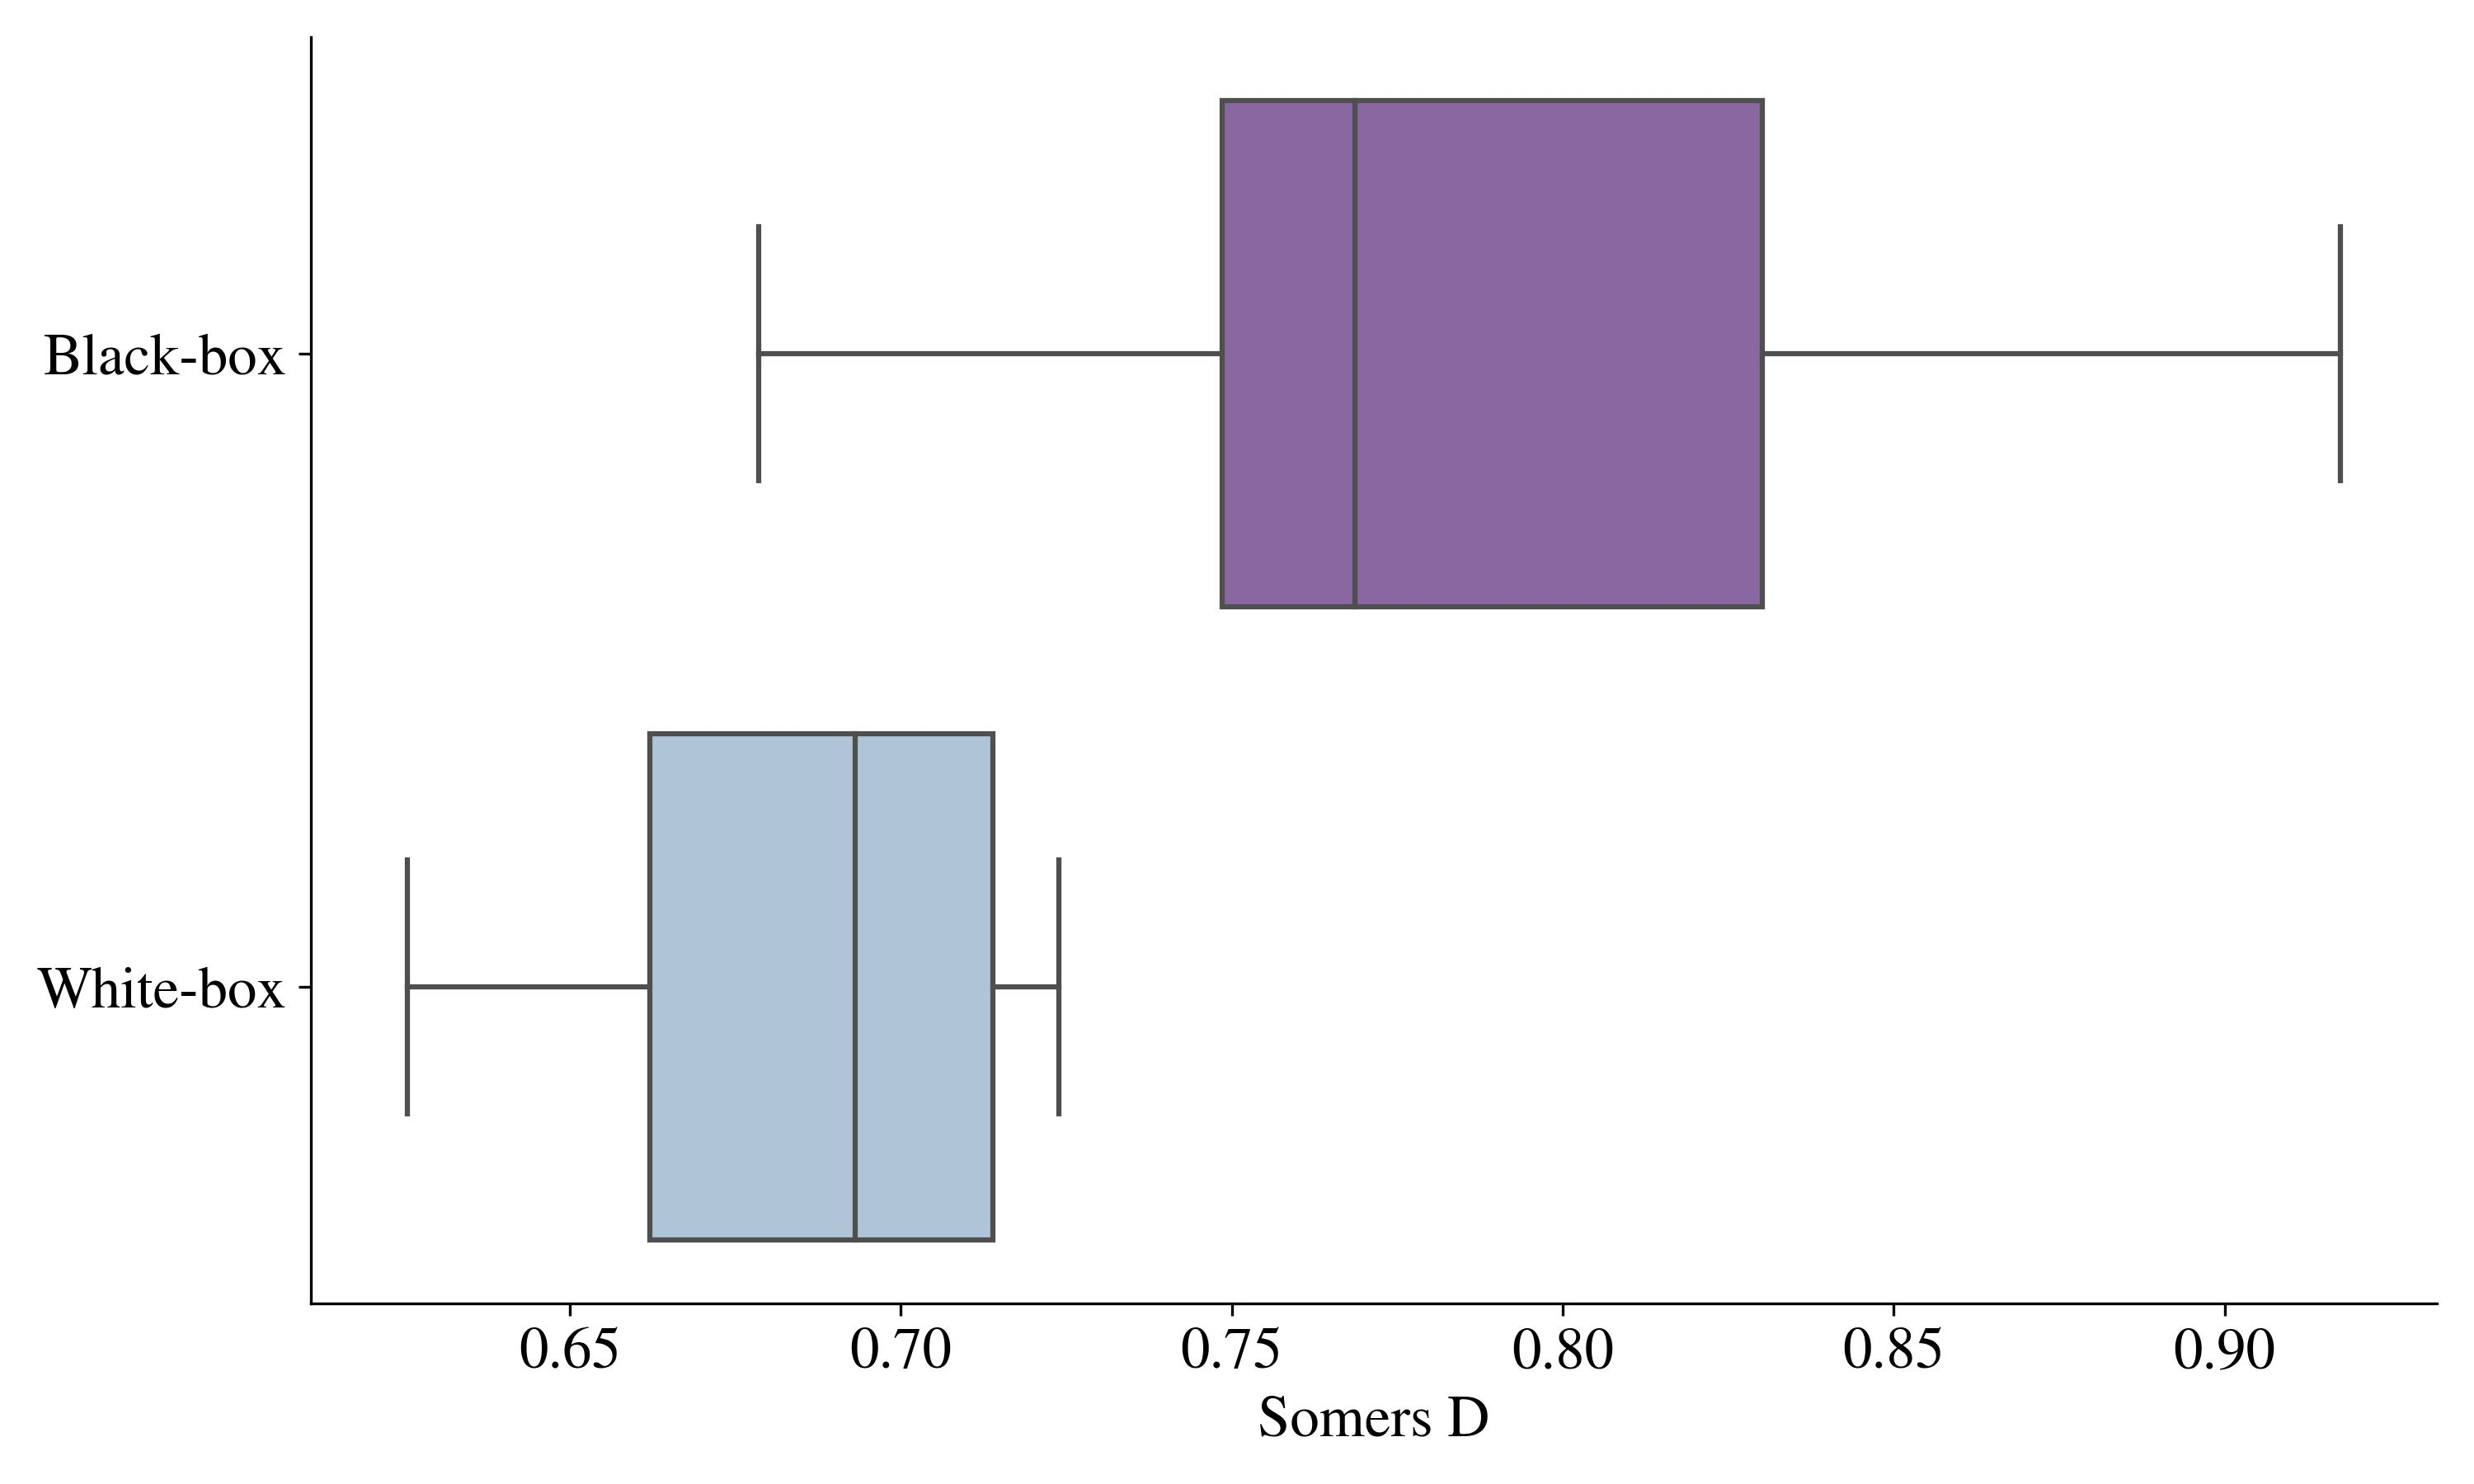
\includegraphics[width=140mm]{Figures/SOMERS D_Distribution_BB_WB.jpg}
    
    \centering{\begin{source}Author's results in Python\end{source}}\vspace{-1em}
\end{figure}